\documentclass[11pt,a4paper,twoside]{thesis}

\usepackage[utf8]{inputenc}
\usepackage{csquotes}
\usepackage[style=numeric-comp, backend=biber]{biblatex}
\usepackage{graphicx}
\usepackage[spanish]{babel}
\usepackage[left=3cm,right=3cm,bottom=3.5cm,top=3.5cm]{geometry}
\usepackage{titlesec}
\usepackage{minted}
\usepackage{listings}
\usepackage{hyperref}
\usepackage{amsmath}
\usepackage{amssymb}
\usepackage{enumitem}
\usepackage{booktabs}
\usepackage{float}
\usepackage{enumitem}
\usepackage{xcolor} % to access the named color LightGray
\setlist{noitemsep} % Elimina el espacio extra entre items
\definecolor{LightGray}{gray}{0.95}
\addbibresource{cites.bib} % Carga el archivo .bib
\bibliography{cites}

\begin{document}

%%%% CARATULA

\def\autor{Adrian Norberto Marino}
\def\tituloTesis{Chatbot para la recomendación personalizada de contenido}
\def\runtitulo{Resumen}
\def\runtitle{Chatbot para la recomendación personalizada de contenido}
\def\director{Roberto Abalde}

\def\lugar{Buenos Aires, Argentina, 2025}

% -----------------------------------------------------------------------------
% Caratula,  Resumen, agradecimientos y dedicatoria.
% -----------------------------------------------------------------------------
\newcommand{\HRule}{\rule{\linewidth}{0.2mm}}
%
\thispagestyle{empty}

\begin{center}\leavevmode

	\vspace{-2cm}

	\begin{tabular}{l}
		
\includegraphics[width=4.6cm]{./images/logouba.png}
	\end{tabular}

	{\large \sc Universidad de Buenos Aires\\Facultad de Ciencias Exactas y Naturales \\ Facultad de Ingeniería}

	\vspace{5.0cm}

	\begin{huge}
		\textbf{\tituloTesis}
	\end{huge}

	\vspace{2cm}

	{\large Traba de tesis de la \textit{Maestría en Explotación de Datos y Descubrimiento del Conocimiento}}
	\vspace{2cm}

	{\large \href{https://github.com/adrianmarino/thesis-paper}{Proyecto en Gihub}}

	\vspace{2cm}

	{\Large \autor}

\end{center}

\vfill

{\large

	{Director: \director}

	\vspace{.2cm}

	\lugar
}

\newpage\thispagestyle{empty}

%
\frontmatter
\pagestyle{empty}
%\begin{center}
%\large \bf \runtitulo
%\end{center}
%\vspace{1cm}
\chapter*{\runtitulo}

\noindent Este trabajo de tesis experimenta con el uso de grandes modelos de lenguaje (\textit{Large language Models o LLM}) como interfaz de comunicación con el usuario final. Estos modelos se emplean para la búsqueda de contenido personalizado para el usuario en respuesta a consultas en lenguaje natural. El sistema de recomendaciones es capaz de ofrecer contenido personalizado al usuario y aborda el problema del \textit{Cold start} mediante un \textit{ensamble} de modelos de recomendación basados en contenido, filtros colaborativos y modelos de lenguaje.

\bigskip

\noindent\textbf{Palabras claves:} \textit{LLM}, \textit{Cold Start}, Sistemas de recomendación basados en Filtro Colaborativos, Sistemas de recomendación en basados en contenido, \textit{API}, \textit{RAG}, \textit{ChromaDB}, \textit{Apache Airflow}, \textit{Llama}, Máquinas de factorización profundas (\textit{DeepFM}).
%
%\cleardoublepage
%\chapter*{Agradecimientos}

\noindent  % OPCIONAL: comentar si no se quiere
%
\cleardoublepage
\chapter*{Agradecimientos}

\hfill \textit{Principalmente a mis padres, siempre fueron un gran apoyo en mi carrera, alentándome incansablemente para seguir adelante en todo momento. Gran parte de mi disciplina de constante persistencia se la debo a ellos. En segundo lugar a mis profesores de la especialización y maestría, por entregarnos su conocimiento dia a dia, siempre enfocados en que comprendamos todos los temas expuesto de la mejor forma posible. A mis compañeros de la especialización, siempre fueron un gran grupo de apoyo, un grupo en el que nos ayudamos uno al otro para comprender los temas expuestos.}
  % OPCIONAL: comentar si no se quiere
% -----------------------------------------------------------------------------
%
%
%
%\cleardoublepage
\tableofcontents
%
%
\mainmatter
\pagestyle{headings}
%
%
%
%
% -----------------------------------------------------------------------------
% Contenido de la tesis
% -----------------------------------------------------------------------------

\chapter{Introducción}

En la era digital actual, la personalización de contenido se ha convertido en un aspecto crucial para mejorar la experiencia del usuario en diversas plataformas de entretenimiento y servicios en línea. Este trabajo de investigación se centra en el desarrollo de un \textit{chatbot} innovador para la recomendación personalizada de contenido, específicamente enfocado en películas, utilizando técnicas avanzadas de procesamiento de lenguaje natural y sistemas de recomendación. Basándose en investigaciones previas \cite{chatrec}, este trabajo busca expandir y mejorar estos conceptos mediante la implementación de un sistema de recomendación que combina grandes modelos de lenguaje (en inglés \textit{Large Language Model} o simplemente \textit{LLM}) con técnicas basadas filtrado colaborativo y contenido.
Esta propuesta se distingue por su enfoque en la utilización de modelos de lenguaje de código abierto, que pueden ejecutarse en máquinas de especificaciones medias, en contraste con los servicios de \textit{API} comerciales utilizados en otros trabajos  \cite{chatrec}. Este enfoque no solo reduce los costos asociados, sino que también permite una mayor flexibilidad y control sobre el proceso de recomendación.
Este trabajo no solo busca mejorar la precisión de las recomendaciones, sino también explorar cómo los grandes modelos de lenguaje pueden enriquecer la experiencia del usuario al proporcionar recomendaciones más contextuales.
A lo largo de este documento, se detallará la arquitectura del sistema, los flujos de inferencia y entrenamiento, los modelos utilizados, y se presentarán los resultados obtenidos. Finalmente, se discutirán las implicaciones de este enfoque y posibles direcciones para futuras investigaciones en el campo de los sistemas de recomendación basados en \textit{chatbots}.

En trabajos previos, se abordaron distintas líneas de investigación con las que se busca mejorar la experiencia de usuario con los sistemas de recomendación mediante el uso de los denominados grandes modelos de lenguaje. El trabajo \textit{ChatREC} \cite{chatrec} aborda el uso de un \textit{LLM}, con el cual el usuario puede entablar una conversación para realizar la búsqueda de contenido personalizado. Basándose en el perfil del usuario y su historial de conversaciones, el modelo realiza recomendaciones de acuerdo a lo que solicite el usuario mediante lenguaje natural. El trabajo mencionado \cite{chatrec} utiliza \textit{LLM}'s a los cuales se puede acceder como un servicio por medio de una \textit{API} de pago, como aquellas ofrecidas por \textit{OpenAI}, \textit{Anthropic} o \textit{DeepSeek} entre otras.

Este trabajo de investigación busca aplicar esta misma técnica utilizando uno o más sistemas de recomendación y grandes modelos de lenguaje de código abierto. Entonces, se busca aplicar la misma técnica utilizando grandes modelos de lenguaje de código abierto, que puedan correr tanto en una máquina virtual o real, de especificaciones medias. Finalmente, se buscara llegar a resultados similares bajo condiciones análogas.

Por otro lado, se definió el alcance de la solución basada en las diferencias entre los grandes modelos de lenguaje utilizados anteriormente \cite{chatrec} y los modelos de código abierto aplicados en este trabajo. A continuación se exponen los lineamiento de este alcance:

\begin{itemize}
	\setlength{\itemsep}{3pt}

	\item Desarrollar un \textit{API} \textit{Rest} para interactuar y configurar el \textit{chatbot} de manera sencilla, permitiendo su integración con sistemas existentes.
	\item El \textit{chatbot} permite crear un perfil de usuario, el cual contiene información inicial del mismo. Esta información ayuda al \textit{chatbot} a realizar recomendaciones basadas en preferencias como el género de las películas y datos del propio usuario. Esto permite abordar el problema del arranque en frío en sistemas de recomendación colaborativa, donde el sistema aun no tiene información sobre el comportamiento del usuario, ya que este no aun no ha interactuado con el mismo.
	\item El \textit{chatbot} permite a los usuarios hacer preguntas en lenguaje natural sobre el contenido que desean ver (películas en este caso) y responde con una lista de películas ordenadas según sus preferencias iniciales o su comportamiento en la plataforma.
	\item Los usuarios pueden calificar las películas que han visto. Estas calificaciones son utilizadas por el \textit{chatbot} para ajustar las recomendaciones futuras a las nuevas preferencias del usuario. Esto significa que la personalización de las recomendaciones depende de la cantidad de calificaciones que el usuario proporcione a la plataforma, afectando tanto el orden de las recomendaciones como el tipo de contenido presentado.
\end{itemize}

\chapter{Modelo de datos y análisis exploratorio}

Para realizar este trabajo se ha seleccionado el dominio del cine, ya que existen
conjuntos de datos bien definidos y actualizados. Estos conjuntos de datos en
general están diseñados específicamente para probar modelos de recomendación. Por otro lado, es
el dominio clásico seleccionado para realizar \textit{papers}, \textit{benchmarks} y literatura de sistemas de recomendación
en general.

Dada la propuesta particular de este trabajo, fue necesario contar con datos referentes a las
interacciones de los usuarios con ítems (películas en este caso). Por otro lado, no fue necesario tener información previa de los usuarios, ya que los perfiles de los usuarios son ingresados por el propio usuario a la plataforma. De esta forma, se reutilizó la base de usuario, ítem e interacciones seleccionada en el trabajo de especialización \cite{src} para obtener la interacciones e items. Por otro lado, los perfiles de los usuario no son necesarios en la etapa de entrenamiento de los modelos, solo para la inferencia, por eso no forman parte del conjunto de datos inicial de entrenamiento.

\section{El conjunto de datos \textit{MovieLens 25M}}

El conjunto de datos \textit{MovieLens 25M}~\cite{movielens} es una colección ampliamente utilizada en el ámbito de la investigación y el desarrollo de sistemas de recomendación. Fue creado por el \textit{GroupLens Research Lab} de la Universidad de \textit{Minnesota} y contiene datos relacionados con películas, calificaciones de usuarios y etiquetas (\textit{tags}) aplicadas por los usuarios. Este conjunto de datos prácticamente no tiene características
para los ítems (películas), pero sí tiene las calificaciones realizadas por los
usuarios sobre los mismos. También cuenta con un conjunto de etiquetas(\textit{tags)} o palabras clave
cargadas por los usuarios para cada ítem (película). Otro punto importante, es
que todos los usuarios tienen al menos $20$ interacciones, lo cual asegura no
tener problemas de bajo rendimiento por falta de estas. De esta forma,
este conjunto de datos sera muy útil para entrenar modelos de recomendación
basados en filtros colaborativos.

Por último, este conjunto de datos contiene $25$ millones calificaciones, $1$
millón de \textit{tags} y $62.423$ películas. Estos datos fueron registrados
por $162.541$ usuarios entre el $9$ de enero de $1995$ y el $21$ de noviembre
de $2019$. A continuación en la tabla~\ref{table:movieLensColumns}, se
especifican las columnas del conjunto de datos:

\begin{table}[!htb]
	\centering
	\footnotesize
	\begin{tabular}{l | p{0.8\linewidth}}
		\hline
		Columna            & Descripción                                                                                                                                                                                 \\
		\hline
		\textit{userId}    & Identificador univoco de un usuario.                                                                                                                                                        \\
		\textit{movieId}   & Identificador univoco de una película.                                                                                                                                                      \\
		\textit{timestamp} & Fecha en la cual el usuario calificó el ítem(\textit{movieId}). Es un string con formato año-mes. Existen valores entre 1997-09 y 2019-11 inclusive.                                        \\
		\textit{rating}    & Calificación del usuario. Es un valor discreto numérico: \textit{0.5}, \textit{1}, \textit{1.5}, \textit{2}, \textit{2.5}, \textit{3}, \textit{3.5}, \textit{4}, \textit{4.5} y \textit{5}. \\
		\textit{tags}      & Lista de palabras definidas por cada usuario, para una película. Dicho de otra forma existen N \textit{tags} por cada par usuario-película.                                                 \\
		\hline
	\end{tabular}
	\caption{
		Columnas del conjunto de datos \textit{Movie Lens}, relevantes para este trabajo.
	}
	\label{table:movieLensColumns}
\end{table}

\clearpage

\section{El conjunto de datos \textit{TMDB}}

El conjunto de datos \textit{TMDB (The Movie Database)}~\cite{tmdb} es una colección de datos relacionados con películas, series de televisión y otros contenidos multimedia, extraídos de la base de datos pública de \textit{The Movie Database (TMDB)}. \textit{TMDB} es una plataforma colaborativa que recopila información detallada sobre películas, actores, directores, géneros y más.
El conjunto de datos no tiene calificaciones personalizadas para los ítems como sucede con el conjunto de datos anterior (\textit{MovieLens}), pero si tiene varias características referentes a películas. Este conjunto de datos es utilizado para filtrar los items del conjunto de datos \textit{MovieLens} ~\cite{movielens} y así tener una base de ítems mas rica en características. Estas características luego serán utilizadas en el proceso de búsqueda de ítems por el \textit{chatbot} haciendo uso de la técnica \textit{RAG}(\textit{Retrieval Augmented Generation} o Generación Aumentada por Recuperación) ~\cite{rag} que se explicara mas adelante. El conjunto contiene datos de $5.000$ películas y sus columnas se especifican en la tabla~\ref{table:tmdbColumns} a
continuación:

\begin{table}[!htb]
	\centering
	\footnotesize
	\begin{tabular}{l | p{0.6\linewidth}}
		\hline
		Columna                                   & Descripción                                                                           \\
		\hline
		\textit{imdb\_id}                         & Identificador univoco de una película en la base de datos de \textit{IMDB}.           \\
		\textit{title y original\_title}          & Título y título original.                                                             \\
		\textit{release\_date}                    & Fecha de estreno.                                                                     \\
		\textit{status}                           & Define si la película fue estrenada o esta en desarrollo.                             \\
		\textit{overview}                         & Sinopsis de la película.                                                              \\
		\textit{poster\_path}                     & URL de imagen de portada de la película.                                              \\
		\textit{languages}                        & Lenguaje original y doblaje.                                                          \\
		\textit{genres}                           & Géneros.                                                                              \\
		\textit{adult}                            & ¿Solo es apta para adultos?                                                           \\
		\textit{popularity}                       & Índice de popularidad.                                                                \\
		\textit{vote\_count}                      & Cantidad de votos.                                                                    \\
		\textit{vote\_average}                    & Promedio de votos.                                                                    \\
		\textit{keywords/tagline} y \textit{tags} & \textit{tags} o palabras clase ingresadas por los usuarios para definir una película. \\
		\textit{budget}                           & Presupuesto destinado a la realización de la película.                                \\
		\textit{revenue}                          & Retorno de inversión o ganancias.                                                     \\
		\textit{production\_companies}            & Compañías que produjeron la película.                                                 \\
		\textit{production\_countries}            & Países donde se produjo la película.                                                  \\
		\textit{homepage}                         & Sitio web oficial.                                                                    \\

		\hline
	\end{tabular}
	\caption{
		Columnas del conjunto de datos \textit{TMDB}, relevantes para este trabajo.
	}
	\label{table:tmdbColumns}
\end{table}

\clearpage

\section{Preprocesamiento de datos}
\label{sec:pre-pro}



Como parte inicial de la etapa de pre-procesamiento de datos, se utilizo una base de datos \textit{MongoDB}. Se uso \textit{MongoDB} y no \textit{Pandas}, dado que \textit{Pandas} requiere cargar todo el conjunto de datos en memoria \textit{RAM}. Si bien se podría lidiar con este problema, aumentado el tamaño de la memoria \textit{Swap} (Linux) o la memoria
virtual (\textit{Windows}), podría ocasionar caídas de procesos y lentitudes innecesarias. En este caso, se selecciono una base de datos de tipo documento, la cual no necesita cargar todos los datos en memoria y por otro lado, existe la posibilidad de escalar la base de datos a mas nodos en caso de ser necesario. Ambos conjuntos de datos contienen varios archivos \textit{csv}, los cuales vamos a llamar \textit{tablas}. En la tabla~\ref{table:tableRatings} se
especifican las columnas utilizadas:

\begin{table}[!htb]
	\centering
	\footnotesize
	\begin{tabular}{l | p{0.75\linewidth}}
		\hline
		File                     & Descripción                                                                                                                                               \\
		\hline

		\textit{movie\_metadata} & Pertenece al conjunto de datos \textit{TMDB}. Es la fuente de verdad de la cual se toman columnas referentes a características de una película.           \\
		\textit{tags}            & Pertenece al conjunto de datos \textit{Movie Lens}. De esta tabla se tomaron los tags o palabras clave dadas de alta por los usuarios por cada película.  \\
		\textit{ratings}         & Pertenece al conjunto de datos \textit{Movie Lens}. De esta tabla se tomaron las calificaciones de los usuario para las películas que fueron calificadas. \\
		\hline
	\end{tabular}
	\caption{
		\textit{files} o tablas utilizadas en este trabajo, para construir un conjunto de datos unificado, el cual sirve como base para entrenamiento y evaluación de modelos.
	}
	\label{table:tableRatings}
\end{table}

Para iniciar, se realizo un \textit{merge} o \textit{join} de las tablas
\textit{ratings} y \textit{tags} por las columnas \textit{user\_id} y
\textit{movie\_id}, ya que tenemos dos columnas que representan interacciones
de usuarios:

\begin{itemize}
	\item \textit{rating}: Pertenece a la tabla \textit{ratings}.
	\item \textit{tags}: Pertenece a la tabla \textit{tags}.
\end{itemize}

En segundo lugar, se realizo un \textit{merge} entre las tablas
\textit{ratings\_tags\_v1} y \textit{movie\_metadata} utilizando la columna
\textit{imdb\_id}, la cual es identificador unívoco de una película en ambas
tablas.

Finalmente, se obtienen dos tablas/\textit{files} como resultado:

\begin{table}[!htb]
	\centering
	\footnotesize
	\begin{tabular}{l | p{0.75\linewidth}}
		\hline
		Filename                       & Descripción                                                                                                                             \\
		\hline
		\textit{movies\_v4.csv}        & Contente toda la información de las películas, incluidos todos los \textit{tags} cargados por los usuarios que calificaron un película. \\
		\textit{ratings\_tags\_v1.csv} & Contiene tanto las calificaciones como los \textit{tags} para cada usuario y película.                                                  \\
		\hline
	\end{tabular}
	\caption{
		\textit{files} resultado del pre-procesamiento. Estos forman parte del conjunto de datos de entrenamiento y evaluación en este trabajo practico.
	}
	\label{table:tableFiles}
\end{table}

\subsection{Tabla de interacciones}

La tabla \textit{ratings\_tags\_v1}~\ref{table:interactionsTableDef} tiene
datos a nivel interacción usuario-ítem. De esta forma, a nivel usuario-ítem se
cuenta con la calificación de la película realizada por el usuario, ademas de
los \textit{tags} que el usuario cargo para esa películas. Estos \textit{tags}
no son mas que una lista de palabras representativas de la película en
cuestión. Por ejemplo, para la película \textit{Toy Story} deberíamos encontrar
palabras referentes a la misma como: \textit{boss}, \textit{woody}, \textit{animation},
\textit{3d}, etc.. Finalmente, contamos con la fecha en la cual se realizaron
esta interacciones. Se entiende que la calificación y los \textit{tags} se
ingresaron en el mismo momento.

\begin{table}[!htb]
	\centering
	\footnotesize
	\begin{tabular}{l | p{0.8\linewidth}}
		\hline
		Columna            & Descripción                                                                                                                                                                     \\
		\hline

		\textit{user\_id}  & Existen $13.281$ usuarios.                                                                                                                                                      \\
		\textit{movie\_id} & Existen $33.444$ películas.                                                                                                                                                     \\
		\textit{timestamp} & Fecha en la cual el usuario califico el ítem(\textit{movie\_id}). Es un \textit{string} de formato año-mes. Existen valores entre 1997-09 y 2019-11 inclusive.                  \\
		\textit{rating}    & Calificación. Es un valor discreto numérico: \textit{0.5}, \textit{1}, \textit{1.5}, \textit{2}, \textit{2.5}, \textit{3}, \textit{3.5}, \textit{4}, \textit{4.5} y \textit{5}. \\
		\textit{tags}      & Lista de palabras definidas por cada usuario para una película. Se cuenta con los \textit{tags} a nivel usuario-película.                                                       \\
		\hline
	\end{tabular}
	\caption{
		Definición de tabla \textit{ratings\_tags\_v1} o tabla de interacciones.
	}
	\label{table:interactionsTableDef}
\end{table}

\subsection{Tablas de metadatos de películas}

La tabla \textit{movies\_v4}~\ref{table:moviesTableDef} cuenta con información
de cada película seleccionada en ambos conjuntos de datos.

\begin{table}[!htb]
	\centering
	\footnotesize
	\begin{tabular}{l | p{0.8\linewidth}}
		\hline
		Columna                   & Descripción                                                                              \\
		\hline

		\textit{title}            & Título de la película.                                                                   \\
		\textit{native\_languaje} & Lenguaje original en el cual fue filmada la película.                                    \\
		\textit{genres}           & Ambos conjuntos de datos cuentan con una lista de géneros a los que adiare la película.  \\
		\textit{overview}         & Sinopsis de la película.                                                                 \\
		\textit{poster}           & Enlaces al detalle de la película en \textit{imdb} y \textit{TMDB}. Estos enlaces
		permiten hace join con mas datos que se encuentren en la descripción de estos
		sitios. En este trabajo solo se utilizara la imagen de la tapa de las película
		a modo de visualización.                                                                                             \\
		\textit{release}          & Fecha de lanzamiento.                                                                    \\
		\textit{budget}           & Presupuesto destinado para la realización el film.                                       \\
		\textit{popularity}       & Popularidad.                                                                             \\
		\textit{vote\_count}      & Cantidad de votos por película.                                                          \\
		\textit{vote\_mean}       & Cantidad media de votos por película.                                                    \\
		\textit{tags}             & Son los \textit{tags} cargados por todos los usuarios que interactuaron con la película.
		Es la mismas información que tenemos en la tabla de interacción pero ahora a nivel ítem.                             \\

		\hline
	\end{tabular}
	\caption{
		Definición de tabla \textit{movies\_v4} o tabla de películas.
	}
	\label{table:moviesTableDef}
\end{table}

\subsection{Valores faltantes}

Una vez generadas ambas tablas, se procedió a buscar \textit{missing values} o
valores faltantes. A continuación, en la tabla~\ref{table:missing-values} se pueden ver
las columnas con valores faltantes:

\begin{table}[h!]
	\centering
	\footnotesize
	\begin{tabular}{lrrrrrr}
		\hline
		Columna     & \% Valores Faltantes \\
		\hline
		budget      & 70                   \\
		poster      & 0.00085              \\
		release     & 0.0085               \\
		popularity  & 0.00085              \\
		vote\_mean  & 4.8                  \\
		vote\_count & 4.6                  \\
		\hline
	\end{tabular}
	\caption{Porcentaje de valores faltantes por columna en la \textit{tabla movies\_v4}.}
	\label{table:missing-values}
\end{table}

Luego se removieron las filas de la tabla ~\ref{table:missing-values} para aquellas columnas
que tuvieran hasta \textit{6 \%} de valores faltantes. A continuación
se removió la columna \textit{budget} por tener un porcentaje muy alto de
valores faltantes, lo que la volvió inutilizable. Por otro lado, la tabla
\textit{ratings\_tags\_v1} no se modifico, ya que no tenia valores faltantes en
ninguna de sus columnas.

Por otro lado, se encontraron valores faltantes en los campos \textit{genres} y \textit{overview}. Aunque no eran nulos, tenían marcadores de ausencia de información, como \textit{"(no genres listed)"} en el campo \textit{genres} y \textit{"No overview found"} en el campo \textit{overview}. Se identificaron \textit{127} ítems sin \textit{overview}, de los cuales se completaron \textit{96}, dejando \textit{31} sin este dato. En el campo \textit{genres}, había \textit{286} ítems con valores faltantes; se llenaron \textit{245}, resultando en \textit{41} sin género asignado. Existían \textit{6581} ítems con un solo género, de los cuales \textit{2531} se actualizaron a dos o más géneros, dejando \textit{4050} con un único género. Para completar los valores faltantes en \textit{overview} y \textit{genres}, se creó un script que extrae datos de un servicio REST proporcionado por la \textit{API} de \textit{TDMB}. Los campos \textit{title}, \textit{overview} y \textit{genres} son fundamentales para el proceso de búsqueda por cercanía(utilizando la técnica \textit{RAG}(\textit{Retrieval Augmented Generation} o Generación Aumentada por Recuperación) ~\cite{rag} en la base de embeddings de la \textit{API Rec Chatbot}. Por esta cuestion se invirtion tiempo en completar la maxima cantidad de missing values para los campos


\subsection{Base datos de interacciones}

Hasta este momento, se contaba con las tablas \textit{ratings\_tags\_v1.csv} y \textit{movies\_v4.csv}. Con base en estas tablas, se generó una base de datos inicial para \textit{API Rec Chatbot}. Se extrajeron los datos necesarios para poblar dos colecciones en la instancia de base de datos \textit{MongoDB} de \textit{API Rec Chatbot}: \textit{interactions} e \textit{items}. Es importante mencionar que se realizó un \textit{merge join} entre las tablas \textit{ratings\_tags\_v1.csv} y \textit{movies\_v4.csv} generando la tabla \textit{rec\_chat\_bot\_data.csv} para asegurar que las interacciones incluyeran items con datos completos, como \textit{title, overview, genres, etc}.

La tabla \textit{rec\_chat\_bot\_data.csv} contiene interacciones virtuales que se utilizarán para entrenar
los modelos del \textit{API Rec Chatbot}, sin estar asociadas a ningún usuario real. Esta base datos es fundamental
para el modelo de filtros colaborativos ya que contiene metadatos de los usuarios y sus interacciones con cada item.
Aunque se podría optar por utilizar un modelo pre-entrenado y aplicar \textit{transfer learning} con datos reales,
se eligió un enfoque más sencillo para facilitar el desarrollo. Así, la base de datos \textit{MongoDB} incluirá interacciones
tanto virtuales como reales.

\clearpage

\section{Análisis exploratorio}


Una vez realizado el procesamiento de datos, se procedió a realizar un análisis exploratorio de todas la variables relevantes del conjunto de datos construido previamente.
A continuación se analiza cada variable relevante.

\subsection{Variable \textit{Rating}}

A continuación se puede apreciar una diagrama de barras el cual describe la
frecuencia con la que los usuarios califican un ítem, segmentada por cada
posible valor de calificación:

\begin{figure}[h!]
	\centering
	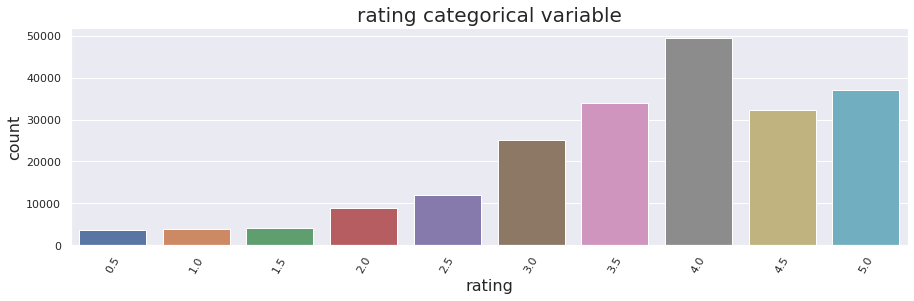
\includegraphics[width=15cm]{./images/rating-barplot.png}
	\caption{Frecuencia o cantidad de observaciones para cada valor discreto de calificación o \textit{rating}.}
	\label{fig:ratingsBarPlot}
\end{figure}

En la figura~\ref{fig:ratingsBarPlot} se puede visualizar que el valor $4.0$
tiene la mayor frecuencia (moda), seguido de $5.0$ puntos y luego $3.5$ puntos.
Por otro lado, se debe tener en cuenta que estas calificaciones provienen de
todo los usuarios. Cada usuario tiene una forma propia de calificar, algunos
tienden a calificar de forma optimista, puntuando con valores altos, y otros
por el contrario, son mas pesimistas y tienden a puntuar con calificaciones
bajas. Este es un comportamiento conocido en el ámbito de sistemas de
recomendación. Se debe tener en cuenta que el valor $3.5$ para un usuario
podría ser un valor $4.5$ para otro. Por otro lado, se aprecia que en general
se tiende a puntuar valores a partir de $3.0$ punto en adelante, habiendo muy
pocas observaciones para puntuaciones menores a los $2.0$ puntos.

\clearpage

Para analizar en mas detalle la variable \textit{rating}, veamos a continuación
un histograma y \textit{boxplot} respectivamente:

\begin{figure}[h!]
	\centering
	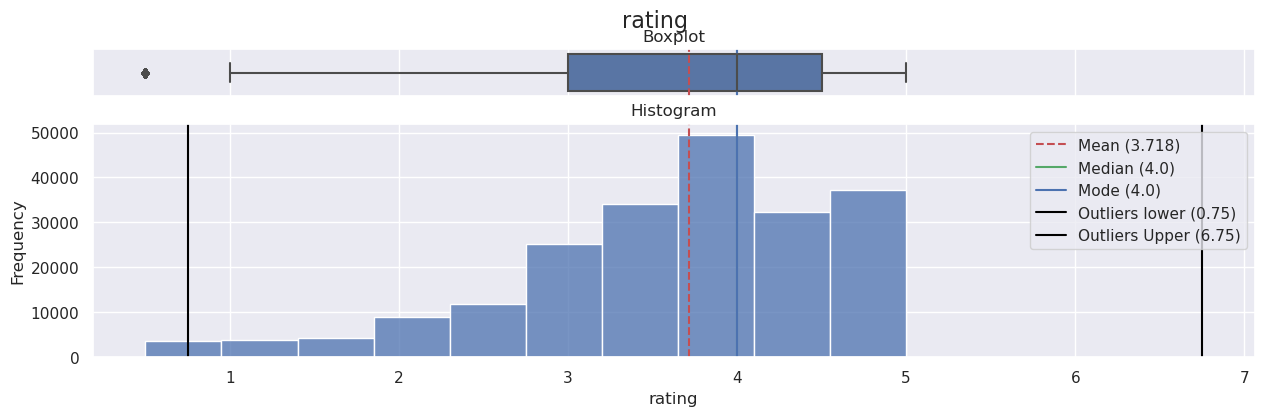
\includegraphics[width=15cm]{./images/rating-boxplot-histplot.png}
	\caption{Histograma y \textit{Boxplot} de la variable \textit{rating}. Los \textit{ratings} son las calificaciones realizadas por los usuario para cada ítem o película.}
	\label{fig:ratingsHistPlot}
\end{figure}

En la figura~\ref{fig:ratingsHistPlot} se aprecia que la variable
\textit{rating} tiene valores discretos entre $0.5$ y $5.0$ con un paso de
$0.5$. De esta forma, contamos con $10$ valores discretos de tipo real, siendo
claramente una variable categórica. Nuevamente vemos algo parecido al diagrama
de barras~\ref{fig:ratingsBarPlot}, el $50\%$ de las observaciones se
encuentran entre los cuantiles $Q1$ y $Q3$ con $3.0$ y $4.5$ puntos (rango
inter-cuantil). La mediana (cuantil $Q2$) esta claramente sobre los $4.0$
puntos, coincidiendo con la moda. La media se encuentra en los $3.5$ puntos a
izquierda de la mediana, debido a que tenemos puntos con frecuencia
considerables a izquierda que mueven a la media en esa dirección. Por otro
lado, tenemos valores atípicos en el extreme izquierdo en los $0.5$ puntos.
Esto se debe a que esta puntuación esta muy alejada del centro de los datos, el
cual se encuentra entre el cuantiles $Q1$ y $Q3$, donde tenemos el $50\%$ las
calificaciones con mayor probabilidad de ocurrencia. No se encuentran valores
atípicos por sobre el máximo. Se puede apreciar un sesgo a izquierda, ya que
existe mayor separación o dispersión de las observaciones entre $Q1$ y $Q2$ que
entre $Q2$ y $Q3$. De esta forma, ambos intervalos conservan su $25\%$ de las
observaciones pero hay menor dispersión entre $Q2$ y $Q3$.

\clearpage
A continuación segmentemos el anterior histograma por año:

\begin{figure}[h!]
	\centering
	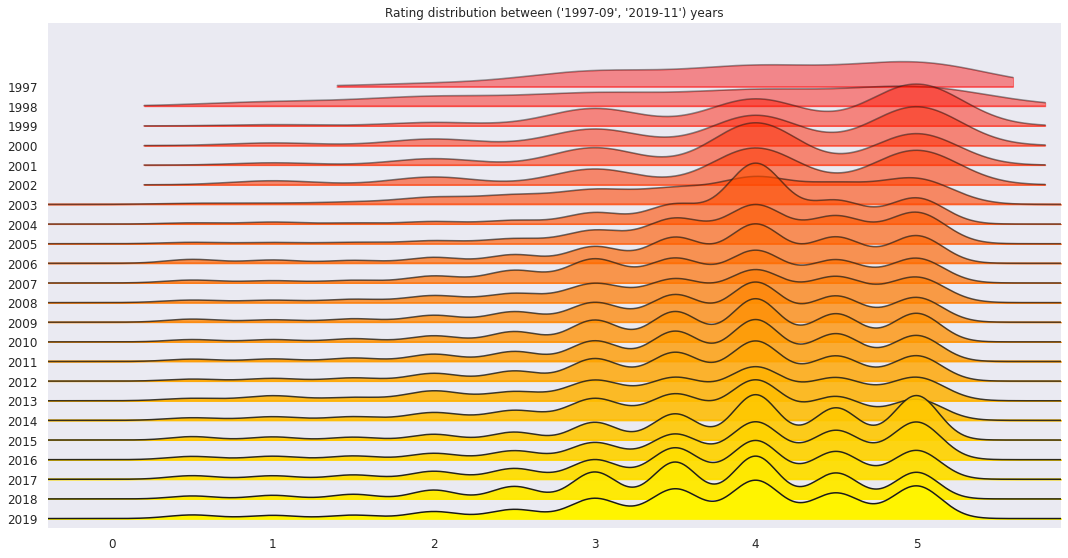
\includegraphics[width=15cm]{./images/rating-by-year.png}
	\caption{
		Histograma de calificaciones segmentado por año.
		En esta gráfica se muestran histogramas como funciones de densidad,
		a pesar de que la variable \textit{rating}
		es categóricas. Las funciones de densidad se graficaron utilizando el
		método de estimación \textit{KDE} o \textit{Kernel Density Estimation}.
		Si bien este método se utiliza para estimar la función de densidad
		de una variable aleatoria continua, en este caso permite apreciar con mayor claridad
		la diferencia en la cantidad de observaciones y el grado de dispersión de cada
		niveles de la variable \textit{rating} por año.
	}
	\label{fig:ratingsYearHistPlot}
\end{figure}

En la figura~\ref{fig:ratingsYearHistPlot} inicialmente vemos que en los años
$1997$, $1998$ y $2003$ la curva tiende a ser mas lineal. Esto indica que la
forma de calificar es mas dispersa, es decir, no se encuentra un perfil de
puntuación claro por parte de los usuarios (si un item es un $4$ o un $5$ por
ejemplo). Entre $1999$ y $2022$ vemos que las puntuaciones $3$, $4$ y $5$ toman
mayor importancia siendo estas las mas utilizadas. Es decir, los usuarios
realizan en su mayoría puntuaciones en esos tres niveles. La mayor frecuencia
se puede ver claramente en los $4$ puntos en el año $2004$, donde fue
prácticamente la mas utilidades decayendo los $3$ y $5$ puntos, en comparación
a años anteriores. A partir del año $2005$ se nota un aumento cada vez más
demarcado en los niveles de puntuaciones entre los $3$ y $5$ puntos, donde los
usuarios cada vez más usan lo niveles $3.5$ y $4.5$. Debemos tener en cuenta
que el aumento en los niveles de puntuación con el tiempo, probablemente sean
debidos a un aumento año a año en la base de usuarios de \textit{Movie Lens} y
tal vez también sea el motivo por el cual en los primeros años vemos mucha
dispersión en las puntuaciones.

\clearpage

\subsection{Correlaciones}

Para realizar un analizar de correlación sobre todas la variables, se realizo
un \textit{merge}-\textit{join} de las tabla \textit{movies} e
\textit{interactions}, incluyendo solamente las columna numéricas. A
continuación podemos visualizar un diagrama de correlación de \textit{Pearson}
de las mismas:

\begin{figure}[h!]
	\centering
	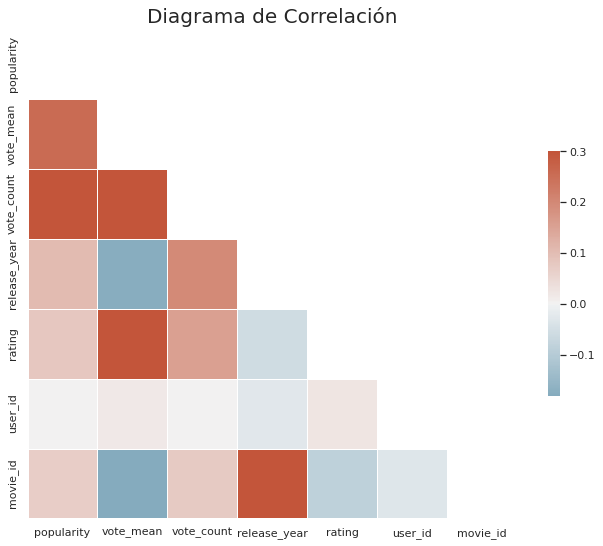
\includegraphics[width=9cm]{./images/Correlations.png}
	\caption{Diagrama de correlación de \textit{Person} aplicado a
		todas las variables numéricas resultado del \textit{merge}
		entre las tablas \textit{movies} e \textit{interactions}.}
	\label{fig:correlationPlot}
\end{figure}

En la figura~\ref{fig:correlationPlot} se aprecia de las variables
\textit{vote\_count}/\textit{vote\_mean} (Cantidad de votos/Media de votos) y
\textit{popularity} (Popularidad) tiene alta correlación debido a que las
películas mas votadas en general son las mas populares. Las variables
\textit{vote\_count} y \textit{vote\_mean} están altamente co-relacionadas
entre si, ya que la media se calcula en base a la variable
\textit{vote\_count}. Por otro lado, también es de esperar que las variables
\textit{rating} (Calificaciones) y la \textit{vote\_mean} estén
co-relacionadas, ya que a medida de aumenta la \textit{vote\_mean} tenemos
calificaciones mas altas. Se encuentra una alta correlación entre la variable
que identifica a una película y la variable \textit{release\_year} (Fecha de
estreno). Esto se debe a que al momento de estrenarse una película, días
después a mas tardar, se da de alta la película en el sitio de \textit{Movie
	Lens}. Esto también nos dice que los identificadores son secuenciales. Las
correlaciones en general son muy bajas llegando a $0.3$ como máximo. Esto es
una buena señal, ya que ayuda a diminuir el fenómeno de co-linealidad de las
variables. Las variables que son combinaciones lineales de otras variables
puede producir que los modelos de \textit{Machine Learning} sobre-ajusten a los
datos de entrenamiento. Las variables \textit{vote\_mean} y \textit{movie\_id}
(Identificador de película) tienen una correlación negativa muy baja. En algún
sentido nos dice que algunas películas mas nuevas tiende a tener una media de
votos menor. Lo mismo sucede entre las variables \textit{rating} y
\textit{movie\_id} en menor medida. Ambas con correlaciones negativas muy
bajas.

Si bien, en esta primera entrega no se están utilizando otras variables
distintas a \textit{user\_id} (Identificador del usuario), \textit{movie\_id} y
\textit{rating}, es de interés analizar las variables correspondiente a
características de películas, ya que en el siguiente entrega (tesis) se planea
implementar modelos de recomendación híbridos, los cuales son ensambles de
sistemas de recomendación basados en contenido y filtros colaborativos.

\subsection{Variables de tipo texto}

Las variables de tipo texto son muy útiles para genera \textit{embeddings}, los
cuales se puede sumar o promediar, generando representaciones compactas de
ítems a recomendar. Luego es posible utilizar estas representaciones para
agrupar ítems según su sinopsis, \textit{tags}, título u otras variables como
pueden ser popularidad, año de estreno, votos, \textit{rating}, etc...

A continuación se puede visualizar la frecuencia de aparición de cada palabra
en cada uno de los campos de tipo texto. Cuanto mayor tamaño tenga la palabra
mayor frecuencia de aparición tendrá.

\begin{description}
	\item[Tags]
\end{description}

Cada usuario puede asociar \textit{tags} o palabras clase a una película. Un
\textit{tag} es una palabra o frase corta que identifica o describe una
película. Es una forma simple de agrupar, ya que los usuarios en general
describen categorías como animación 3d, cual es el director, una frase que
describe algún tipo de categoría o algo relevante en el contenido de la misma.

\begin{figure}[h!]
	\centering
	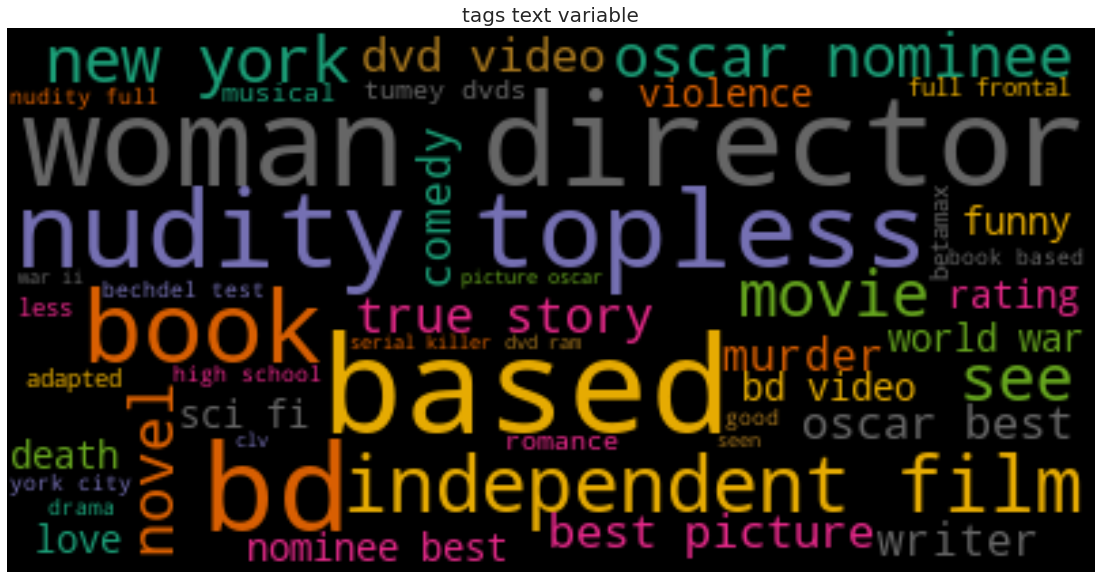
\includegraphics[width=9cm]{./images/Cloud-tags.png}
	\caption{Frecuencia de frases encontradas en la variable \textit{Tags}. El tamaño de cada frase representan la cantidad de apariciones de la misma.}
	\label{fig:tagsCloud}
\end{figure}

En la figura~\ref{fig:tagsCloud} las palabras \textit{based} (basada/o en),
\textit{Book}, \textit{Bd}, \textit{Director}, \textit{Nudity},
\textit{Topless}, \textit{Independent}, \textit{Film}, son aquella palabras mas
cargan por los usuarios en cada película. Otras palabras de menor frecuencia:
\textit{Movie}, \textit{Murder}, \textit{Novel}, \textit{Funny}, \textit{Oscar
	nominee}, \textit{Violent}, \textit{World war}, \textit{True story}.

\clearpage

\begin{description}
	\item[Overview ]
\end{description}

La variable \textit{overview} es la sinopsis de la película. Esta describe
brevemente el contenido de la misma, sin revelar su desenlace.

\begin{figure}[h!]
	\centering
	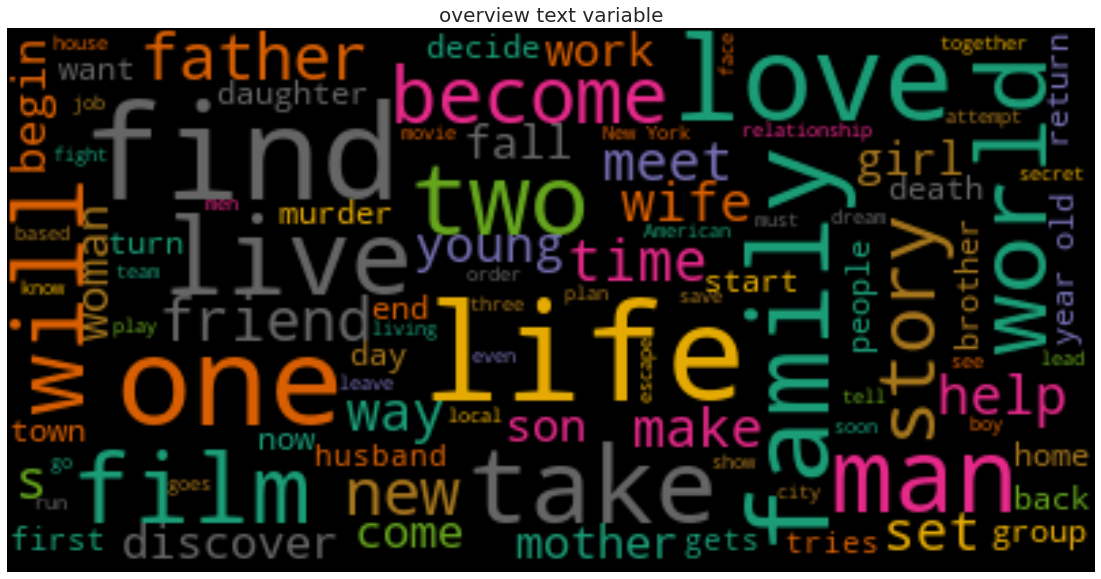
\includegraphics[width=9cm]{./images/Cloud-Overview.png}
	\caption{
		Frecuencia de palabras encontradas en la variable
		\textit{Overview}. El tamaño de cada palabra representan
		la cantidad de apariciones de la misma.
	}
	\label{fig:overviewCloud}
\end{figure}

En la figura~\ref{fig:tagsCloud} podemos visualizar las siguientes palabras con
mayor frecuencia: \textit{Find}, \textit{Live}, \textit{Love}, \textit{Wife},
\textit{One}, \textit{Man}, \textit{Film}, \textit{Become}, \textit{Family},
\textit{Story}, \textit{World}, \textit{Work}, \textit{Father}, \textit{New},
\textit{Friend} y \textit{Story}. Se aprecia una diferencia notoria entre las
variables \textit{tags} y \textit{overview}(Sinopsis). La variable
\textit{tags} parece categorizar las películas desde distintas perspectivas.
Por otro lado, la variable \textit{overview} contiene palabras que son mas
utilizadas en la descripción de la misma. A simple vista, los clusters
(\textit{Embeddings}) que pudieran generarse utilizando esta variable, podrían
ser mas específicos que aquellos \textit{clusters} generados a partir de la
variable \textit{tags}.

\begin{description}
	\item[Title]
\end{description}

\begin{figure}[h!]
	\centering
	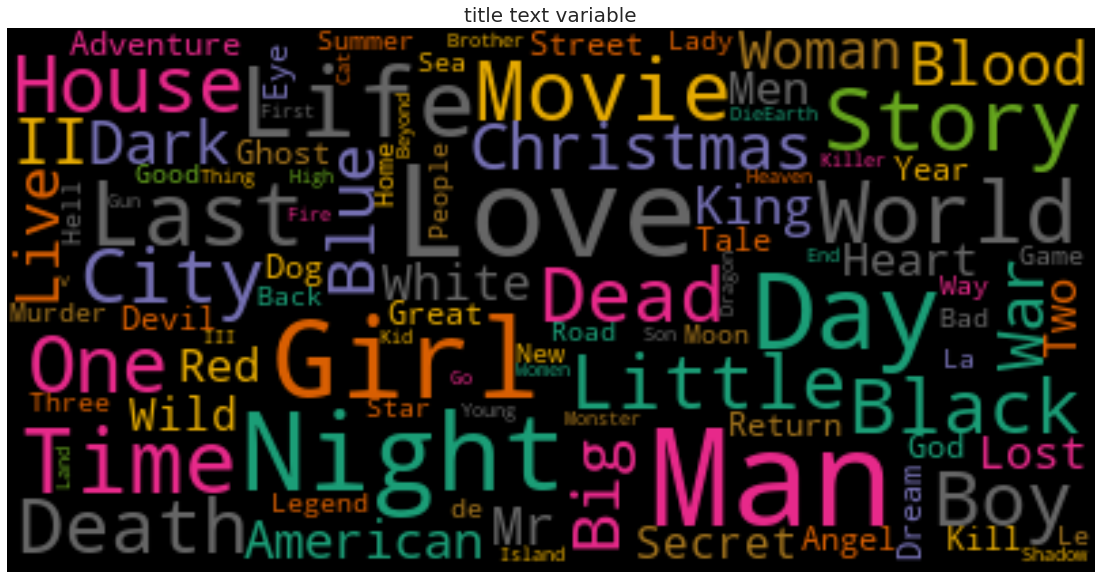
\includegraphics[width=9cm]{./images/Cloud-Title.png}
	\caption{Frecuencia de palabras encontradas en la variable
		\textit{Title}. El tamaño de cada palabra representan la
		cantidad de apariciones de la misma.}
	\label{fig:titleCloud}
\end{figure}

En la figura~\ref{fig:tagsCloud} podemos visualizar las siguientes palabras con
mayor frecuencia: \textit{Girl}, \textit{Man}, \textit{Day}, \textit{Dead},
\textit{Movie}, \textit{Time}, \textit{Night}, \textit{Life}, \textit{House},
\textit{Dark}, \textit{II}, \textit{Blood}, \textit{Christmas}, \textit{World},
\textit{War}, \textit{Black}, \textit{Boy}, \textit{Blue}, \textit{One} y
\textit{King}. A simple vista, una clusterización realizada con esta variable
puede ser mas general que la lograda con la variable \textit{overview}, pero
menos general que la variable \textit{tags}. En trabajos posteriores se
realizaran experimentos para ver resultado en este sentido.

\clearpage

\subsection{Análisis de Componentes Principales}

En esta sección se describe el análisis de componentes principales realizado
sobre las variable numéricas, resultado de fusionar las tablas \textit{movies}
y \textit{interactions}.

\begin{description}
	\item[Varianza Explicada]
\end{description}

Las componentes principales son las variables resultado al aplicar el
algoritmo \textit{PCA}~\cite{pca}. Estas nuevas variables tienen la particularidad de ser
ortogonales entre sí, lo que implica que no poseen ninguna correlación. Además,
a lo largo de todas las variables, la acumulación de varianza disminuye. Esto
indica que la primera componente tiene la mayor varianza y la última la menor
posible (en orden descendente).

\begin{figure}[h!]
	\centering
	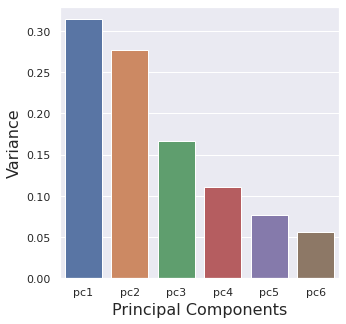
\includegraphics[width=8cm]{./images/PCA-Variance.png}
	\caption{Este diagrama de barras describe el grado de variabilidad o varianza explicada para cada componente principal resultado de aplicar el algoritmo\textit{PCA}~\cite{pca} sobre el conjunto de variables numéricas originales.}
	\label{fig:explainedVariancePlot}
\end{figure}

\begin{description}
	\item[Varianza]
\end{description}
\begin{itemize}
	\item pc1: $31$ \%
	\item pc2: $28$ \%
	\item pc3: $16$ \%
	\item pc4: $11$ \%
	\item pc5: $7$ \%
	\item pc6: $5$ \%
\end{itemize}

En la figura~\ref{fig:explainedVariancePlot}, inicialmente podemos apreciar que
todas las componentes tienen niveles de variabilidad o varianza explicada muy
bajos, donde la primera componente llega solamente al $31$ \%. Esto indica que
el grado de correlación de las variables originales es muy bajo. Utilizando el
criterio del bastón roto podríamos seleccionar las 3 primeras componentes
principales, ya que son las que acumulan mayor varianza.

Por otro lado, debemos tener en cuenta que el análisis por componentes
principales es un análisis lineal. Es decir, tiene encuentra unicamente
correlaciones lineales entre las variables originales. De esta forma, el método
puede estar perdiendo de vista correlaciones no lineales mas complejas, donde
podríamos encontrar un mayor grado de correlación. Las 3 primeras componentes
acumulan un grado de variabilidad del $85$ \%.

\begin{description}
	\item[Cargas o Loadings]
\end{description}

Las componentes principales son combinaciones lineales de las variables
originales. Luego, las cargas o \textit{loadings} son los coeficientes
utilizados para transformar las variables originales en las componentes
principales mediante combinaciones lineales.

De esta forma, los coeficientes definen una medida de correlación o grado de
aporte de cada variable original a una componente principal.

A continuación se pueden visualizar las cargas o \textit{loadings}:

\begin{table}[h!]
	\centering
	\begin{tabular}{lrrrrrr}
		\toprule Variable   & PC1    & PC2   & PC3     \\
		\midrule Popularity & 0.79   & -0.09 & -0.003  \\
		Vote Mean           & 0.55   & -0.55 & -0.03   \\
		Vote Count          & 0.88   & -0.11 & -0.0002 \\
		Release Year        & 0.33   & 0.8   & 0.045   \\
		User ID             & -0.006 & -0.08 & 0.99    \\
		Movie ID            & 0.24   & 0.8   & 0.04    \\
		\bottomrule
	\end{tabular}

	\caption{
		Coeficientes de componentes principales vs variables
		originales. Cada uno de estos valores representan el grado
		de correlación o aporte de cada variable original a
		cada componente principal.
	}
	\label{fig:loadingsTable}
\end{table}

En la tabla~\ref{fig:loadingsTable} vemos que \textit{Vote Count (88\%)}
(Cantidad de votos) y \textit{Popularity (80\%)} (Popularidad) tiene una
correlación positiva muy alta sobre la componente $PC1$. Lo mismo sucede con
\textit{Vote Mean (55\%)} (Media de la cantidad de votos) en menor medida.
Entre dos observaciones con distintos valores de popularidad, la que tenga un
valor mas alto, aportara mas a la componente $PC1$ que a las otra dos ($PC2$ y
$PC3$). También vemos que las variable \textit{Release Year} (Año de estreno) y
\textit{Movie ID} tienen un aporte, considerable, pero mas bajo del 33\% y 24\%
respectivamente, sobre la componente $PC1$. La variable \textit{User ID} no
tiene aporte alguno sobre la componente $PC1$. Las variables que mas aportan a
la componente $PC2$ son \textit{Vote Mean (55\%)} y \textit{Vote Count (11\%)}
respectivamente. Este aporte es negativo, esto indica que un aumento en los
niveles de esta variable significa una disminución en la componente $PC2$. La
variable \textit{Release Year} (Año de estreno) tiene el aporte positivo mas
alto sobre la componente $PC2$ siendo del 80 \%. Para la componente $PC3$, las
variables que mas aportan son \textit{User ID (99\%)} y \textit{Release Year
	(45\%)} respectivamente, ambas positivas. Vemos que un aumento en la variable
\text{User ID} produce un aumento casi en una unidad sobre el coeficiente, pero
\textit{Release Year} es la mitad en relación. De este forma, la componente
$PC1$ podríamos nombrarla como Nivel de popularidad o conocimiento general de
una película. La componente $PC2$, en algún sentido mide lo contrario a la
popularidad, es un indicador de cuan \textit{underground} es un nuevo estrenos.
La componente $PC3$ es mas difícil de nombrar, pero podría llamarse: Grado
\textit{newbie} de un usuario, indicando cuan nuevo es un usuario.

\clearpage

\begin{description}
	\item[\textit{Biplot}]
\end{description}

\begin{figure}[h!]
	\centering
	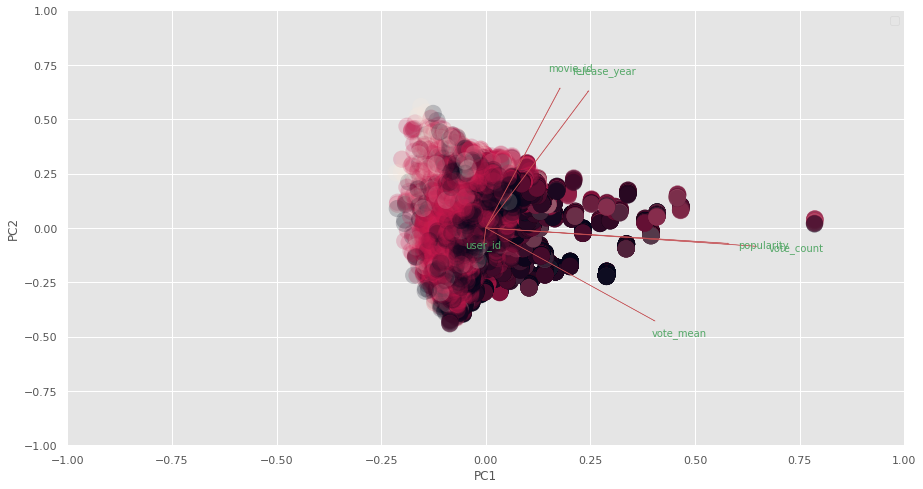
\includegraphics[width=15cm]{./images/PCA-biplot.png}
	\caption{
		Diagrama~\cite{biplot}\textit{Biplot}. Este diagrama representa
		los valores de las variables originales coloreados en color rojo,
		negro y gris. Estos colores corresponden a tres segmentos de
		calificaciones: $>2$, entre $2$ y $3.5$ y $>4$.
		También se pueden apreciar los vectores correspondientes a
		las variables originales.
	}
	\label{fig:biplot}
\end{figure}

En la figura~\ref{fig:biplot} se expone un diagrama
\textit{Biplot}~\cite{biplot}. Este representa los valores de las variables
originales coloreados en color rojo, negro y gris correspondientes a tres
segmentos de calificaciones: $>2$, entre $2$ y $3.5$ y $>4$. También se
representan los vectores correspondientes a las variables originales. A primera
vista observamos que las variables \textit{Popularity} (Popularidad) y
\textit{Vote Count} (Cantidad de votos) tienen una correlación muy alta, ya que
el ángulo entre sus vectores es prácticamente cero. Esto tiene sentido, ya que
ambas son medidas de popularidad de alta co-linealidad. Las variables
\textit{Popularity} (Popularidad), \textit{Vote Count} (Cantidad de votos) y
\textit{Vote Mean} (Media de la cantidad de votos) tiene un aporte positivo
sobre la componente $PC1$ (en menor media). Esto último se corresponde con los
coeficientes de las cargas analizados anteriormente. Las variables
\textit{Movie ID} y \textit{Release Year} (Año de estreno) aportan en menor
medida sobre la componente $PC1$. De esta forma, se constata lo visto
anteriormente en análisis de carga, donde la componente $PC1$ representa el
grado de popularidad de una película. La variable \textit{Vote Mean} (Media de
la cantidad de votos) aporta en forma negativa y las variables \textit{Movie ID
} y \textit{Release Year} (Año de estreno), en forma positiva sobre la
componente $PC2$. Las variables \textit{Popularity} (Popularidad), \textit{Vote
	Count} (Cantidad de votos) tienen casi aporte nulo a la componente $PC2$ en
correspondencia con el análisis de cargas anteriormente expuesto. Si
visualizamos los puntos que representan a las observaciones originales en el
espacio latente generado por \textit{PCA}~\cite{pca}, vemos que las
observaciones de color negro ($>4$ puntos) y gris (entre $2$ y $3.5$ puntos) se
encuentran mas a la derecha que aquellas coloreadas en rojo ($>2$ puntos). Esto
indica que hay un crecimiento del nivel de popularidad cuanto mas a derecha se
encuentre un punto en la componente $PC1$, validando los análisis anteriores.
Si visualizamos lo puntos correspondientes a las observaciones en las
direcciones de la componente $PC2$, vemos que a mayor valor en la componente,
menor es el grado de popularidad de las películas, ya que los puntos rojos
tienden a estar en el extremo positivo de la componente. Esto valida la
hipótesis de que la componente $PC2$ indica cuan \textit{underground} es un
película.


\chapter{Arquitectura General de \textit{Rec Chatbot API}}
\label{sec:arq-general}

Para llevar a cabo este trabajo de investigación, se tomó la decisión de modificar el enfoque tradicional que comúnmente se utiliza para investigar en este ámbito. Por lo general, la metodología típica implica el desarrollo de una librería o paquete en \textit{python}, que resulta ser accesible tanto desde un entorno de \textit{Jupyter} como desde cualquier aplicación que haya sido creada utilizando dicho lenguaje de programación. Sin embargo, en este caso particular, se optó por una alternativa diferente: se decidió crear una \textit{API} que opere bajo un contrato \textit{REST}. Esta elección presenta diversas ventajas significativas en comparación con el desarrollo convencional de una librería o paquete:


\begin{itemize}
	\setlength{\itemsep}{0pt}
	\setlength{\parskip}{0pt}

	\item \textbf{Independencia del lenguaje}: Una \textit{API REST} puede ser consumida por cualquier lenguaje de programación que soporte \textit{HTTP}, no solo \textit{Python} o el lenguaje con el que este escrito el paquete.

	\item \textbf{Escalabilidad}: Las \textit{APIs REST} son más fáciles de escalar horizontalmente, distribuyendo la carga entre múltiples servidores.

	\item \textbf{Separación cliente-servidor}: Permite una clara separación entre el \textit{frontend} y el \textit{backend}, facilitando el desarrollo y mantenimiento de forma independiente.

	\item \textbf{Integración con sistemas distribuidos}: Facilita la integración con otros servicios y sistemas distribuidos.

	\item \textbf{Caching}: Se puede implementar caches fácilmente a nivel \textit{HTTP} para mejorar el rendimiento.

	\item \textbf{Seguridad}: Permite implementar mecanismos de autenticación y autorización estándar como \textit{OAuth} entre otros.

	\item \textbf{Documentación}: Existen herramientas para generar documentación automática de \textit{APIs REST} (como \textit{Swagger}, \textit{Redoc}, \textit{OpenAPI}, etc..).
\end{itemize}

Luego, en la figura \ref{fig:deployment} se pueden apreciar las piezas que componente la arquitectura general de la \textit{API REST} (desde ahora \textit{API Rec Chatbot}).
\vfill

\begin{figure}[H]
	\centering
	\label{fig:deployment}
	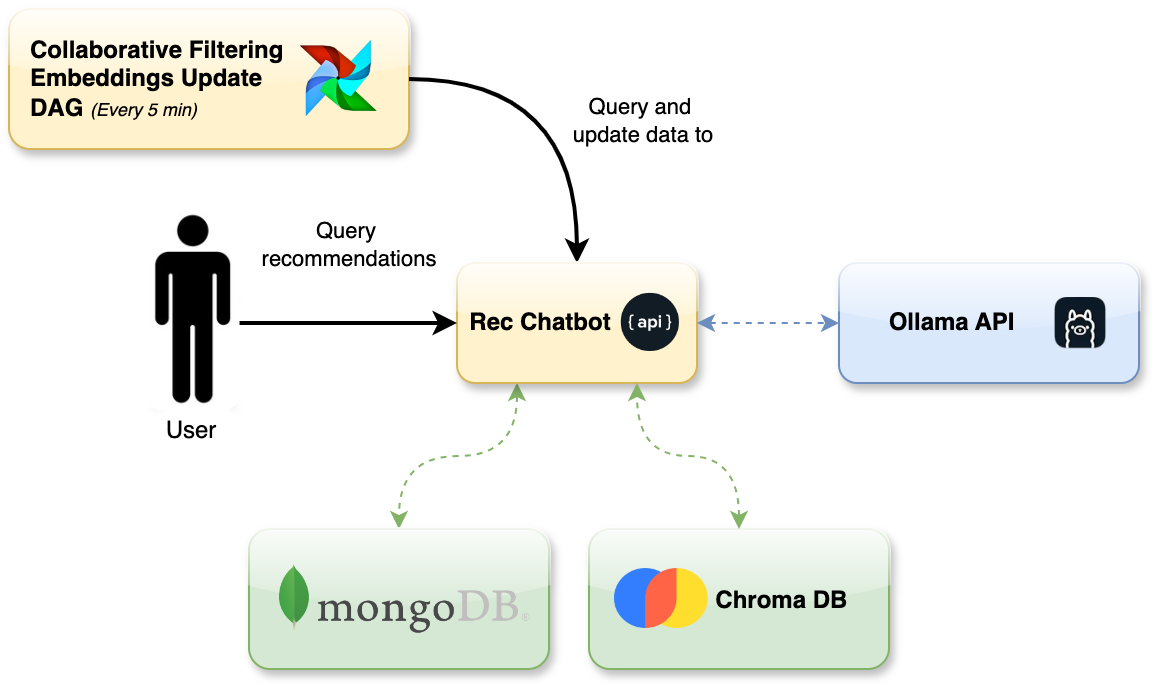
\includegraphics[width=10.5cm]{./images/deployment.png}
	\caption{Arquitectura general: Se puede preciar un diagrama de despliegue donde se especifica cada componente de la arquitectura general y la interacción entre los mismos.}
\end{figure}

En este contexto, puede apreciarse un diagrama de despliegue que ilustra de manera detallada cada uno de los componentes que conforman la arquitectura general y la interacción que existe entre ellos. A grandes rasgos, al inicio del proceso, el usuario realiza una solicitud de recomendaciones utilizando lenguaje natural, lo que inicia una serie de operaciones en el sistema. En este punto, el componente conocido como \textit{API Rec Chatbot} se encarga de buscar ítems que sean relevantes y cercanos a la petición del usuario en una instancia de \textit{ChromaDB}. Una vez que se han encontrado los ítems pertinentes, el sistema procede a realizar un ordenamiento de estos elementos. Este paso es clave, ya que se utilizan tanto los modelos de lenguaje que son proporcionados por \textit{API Ollama} como también los embeddings y las predicciones que son generadas por los modelos de filtros colaborativos, los cuales han sido específicamente entrenados a través de un proceso que se ejecuta en la instancia de \textit{Apache Airflow} \cite{apache-airflow}. Este último proceso asegura que los resultados sean eficaces y relevantes para el usuario. Además, es importante destacar que todos los datos que están relacionados con los perfiles de los usuarios, así como las calificaciones que estos otorgan, las predicciones que se generan, entre otros aspectos importantes, se persisten en una instancia de base de datos \textit{MongoDb}. Esta persistencia de datos es crucial para el funcionamiento continuo y la mejora del sistema, ya que permite realizar un seguimiento de las interacciones y preferencias de los usuarios a lo largo del tiempo.

\vfill
\section{Componentes}

Por un lado, el \textit{API Rec Chatbot} desarrollada en este trabajo, permite gestionar perfiles de usuarios, registrar su historial de calificaciones de películas y ofrecer recomendaciones a través de sus solicitudes en lenguaje natural.

Por otro lado, el \textit{API Rec Chatbot} esta integrada con el \textit{API Rest Ollama} que facilita realizar consultas a una batería de grandes modelos de lenguaje. El \textit{API Rec Chatbot} se enfoca mayormente en la inferencia de recomendaciones mediante un ensamble de modelos o algoritmo de inferencia que combina grandes modelos de lenguaje y modelos de filtros colaborativos en diversas partes de su flujo. Mas adelante, se explicará detalladamente el flujo de inferencia y entrenamiento de la solución.

Para la gestión y operación de \textit{LLM} locales, se eligió la plataforma \textit{Ollama}. Esta herramienta permite a los usuarios descargar modelos \textit{LLM} pre-entrenados que son especialmente receptivos a instrucciones en lenguaje natural, lo cual es crucial para desarrollar aplicaciones interactivas. Una característica destacada de \textit{Ollama} es su capacidad para servir localmente una interfaz \textit{Rest}, que brinda a los desarrolladores acceso fácil y eficiente a todos los modelos de lenguaje descargados.

En cuando al modelo de datos se cuenta separados en dos base de datos:
\begin{itemize}
	\item La primera de estas es una base de datos \textit{MongoDB}. Esta base de datos se encarga de almacenar información relacionada a los perfiles de los clientes que interactúan con la \textit{API Rec Chatbot}. A su vez, también guarda ítems, que en este contexto se refieren a las películas disponibles en el sistema, así como las calificaciones proporcionadas por los usuarios sobre las mismas. Estas calificaciones pueden abarcar tanto datos reales, aquellos introducidos por los propios usuarios, como predicciones generadas por el sistema. De esta forma, se busca ofrecer un servicio personalizado y adaptado a las preferencias de cada usuario.

	\item La segunda es un base de datos \textit{ChromaDB}. Esta base de datos tiene una función específica en el almacenamiento de \textit{embeddings}, que son representaciones vectoriales tanto de los usuarios como de los ítems, ambas generadas por un modelo de filtros colaborativos. Además se almacenan \textit{embeddings} que reflejan el contenido de cada ítem, en este caso, las películas, lo que a su vez habilita la utilización de la técnica conocida como \textit{RAG}(\textit{Retrieval Augmented Generation} o Generación Aumentada por Recuperación) ~\cite{rag}. Esta técnica permite realizar búsquedas de ítems que son similares a las consultas realizadas por los usuarios.
\end{itemize}


Por último, se utilizo una instancia de \textit{Apache Airflow}. \textit{Apache Airflow} permite la orquestación de flujos de trabajo para programar, ejecutar y monitorear secuencias complejas de tareas. Estos procesos se representan como grafos dirigidos acíclicos, lo que facilita dividir un proceso en tareas más simples y re-utilizables. Esto es fundamental para re-entrenar el ensamblaje de modelos del \textit{API Rec Chatbot} y generar las predicciones y embeddings necesarios para su funcionamiento. Además, debido a la significativa cantidad de usuarios, ítems e interacciones en el conjunto de datos, esta arquitectura es esencial para garantizar el correcto funcionamiento del \textit{API Rec Chatbot} y evitar problemas de escalabilidad. En resumen, se trata de una forma de desarrollar aplicaciones que es comúnmente utilizada por empresas de servicios en Internet.

\chapter{Flujo de inferencia de \textit{Rec Chatbot API}}

En la sección anterior se presentó la arquitectura general de la solución, detallando cada componente mediante un diagrama de despliegue, lo que ayuda a entender de forma mas simple la solución. En esta sección, se profundizara en cada uno de estos componentes y explicaremos el funcionamiento de la solución. Para ello, dividiremos la funcionalidad de \textit{API Rec Chatbot} en dos flujos:

\begin{itemize}
	\setlength{\itemsep}{0pt}
	\setlength{\parskip}{0pt}

	\item Flujo de entrenamiento de modelos y generación de datos: Necesarios para la inferencia de \textit{API Rec Chatbot}.
	\item Flujo de inferencia sobre las consultas del usuario: En este flujo se explica el paso a paso, desde que el usuario realiza una consulta, hasta que obtiene una recomendación como respuesta.
\end{itemize}

Comencemos con el flujo de inferencia. En la siguiente figura \ref{fig:inference-flow}, se puede apreciar un diagrama donde se expone el flujo de inferencia. Es decir, cada vez que un usuario realizar una consulta a \textit{API Rec Chatbot} se realizan todas las acciones especificada en este flujo.
\vfill

\begin{figure}[H]
	\centering
	\label{fig:inference-flow}
	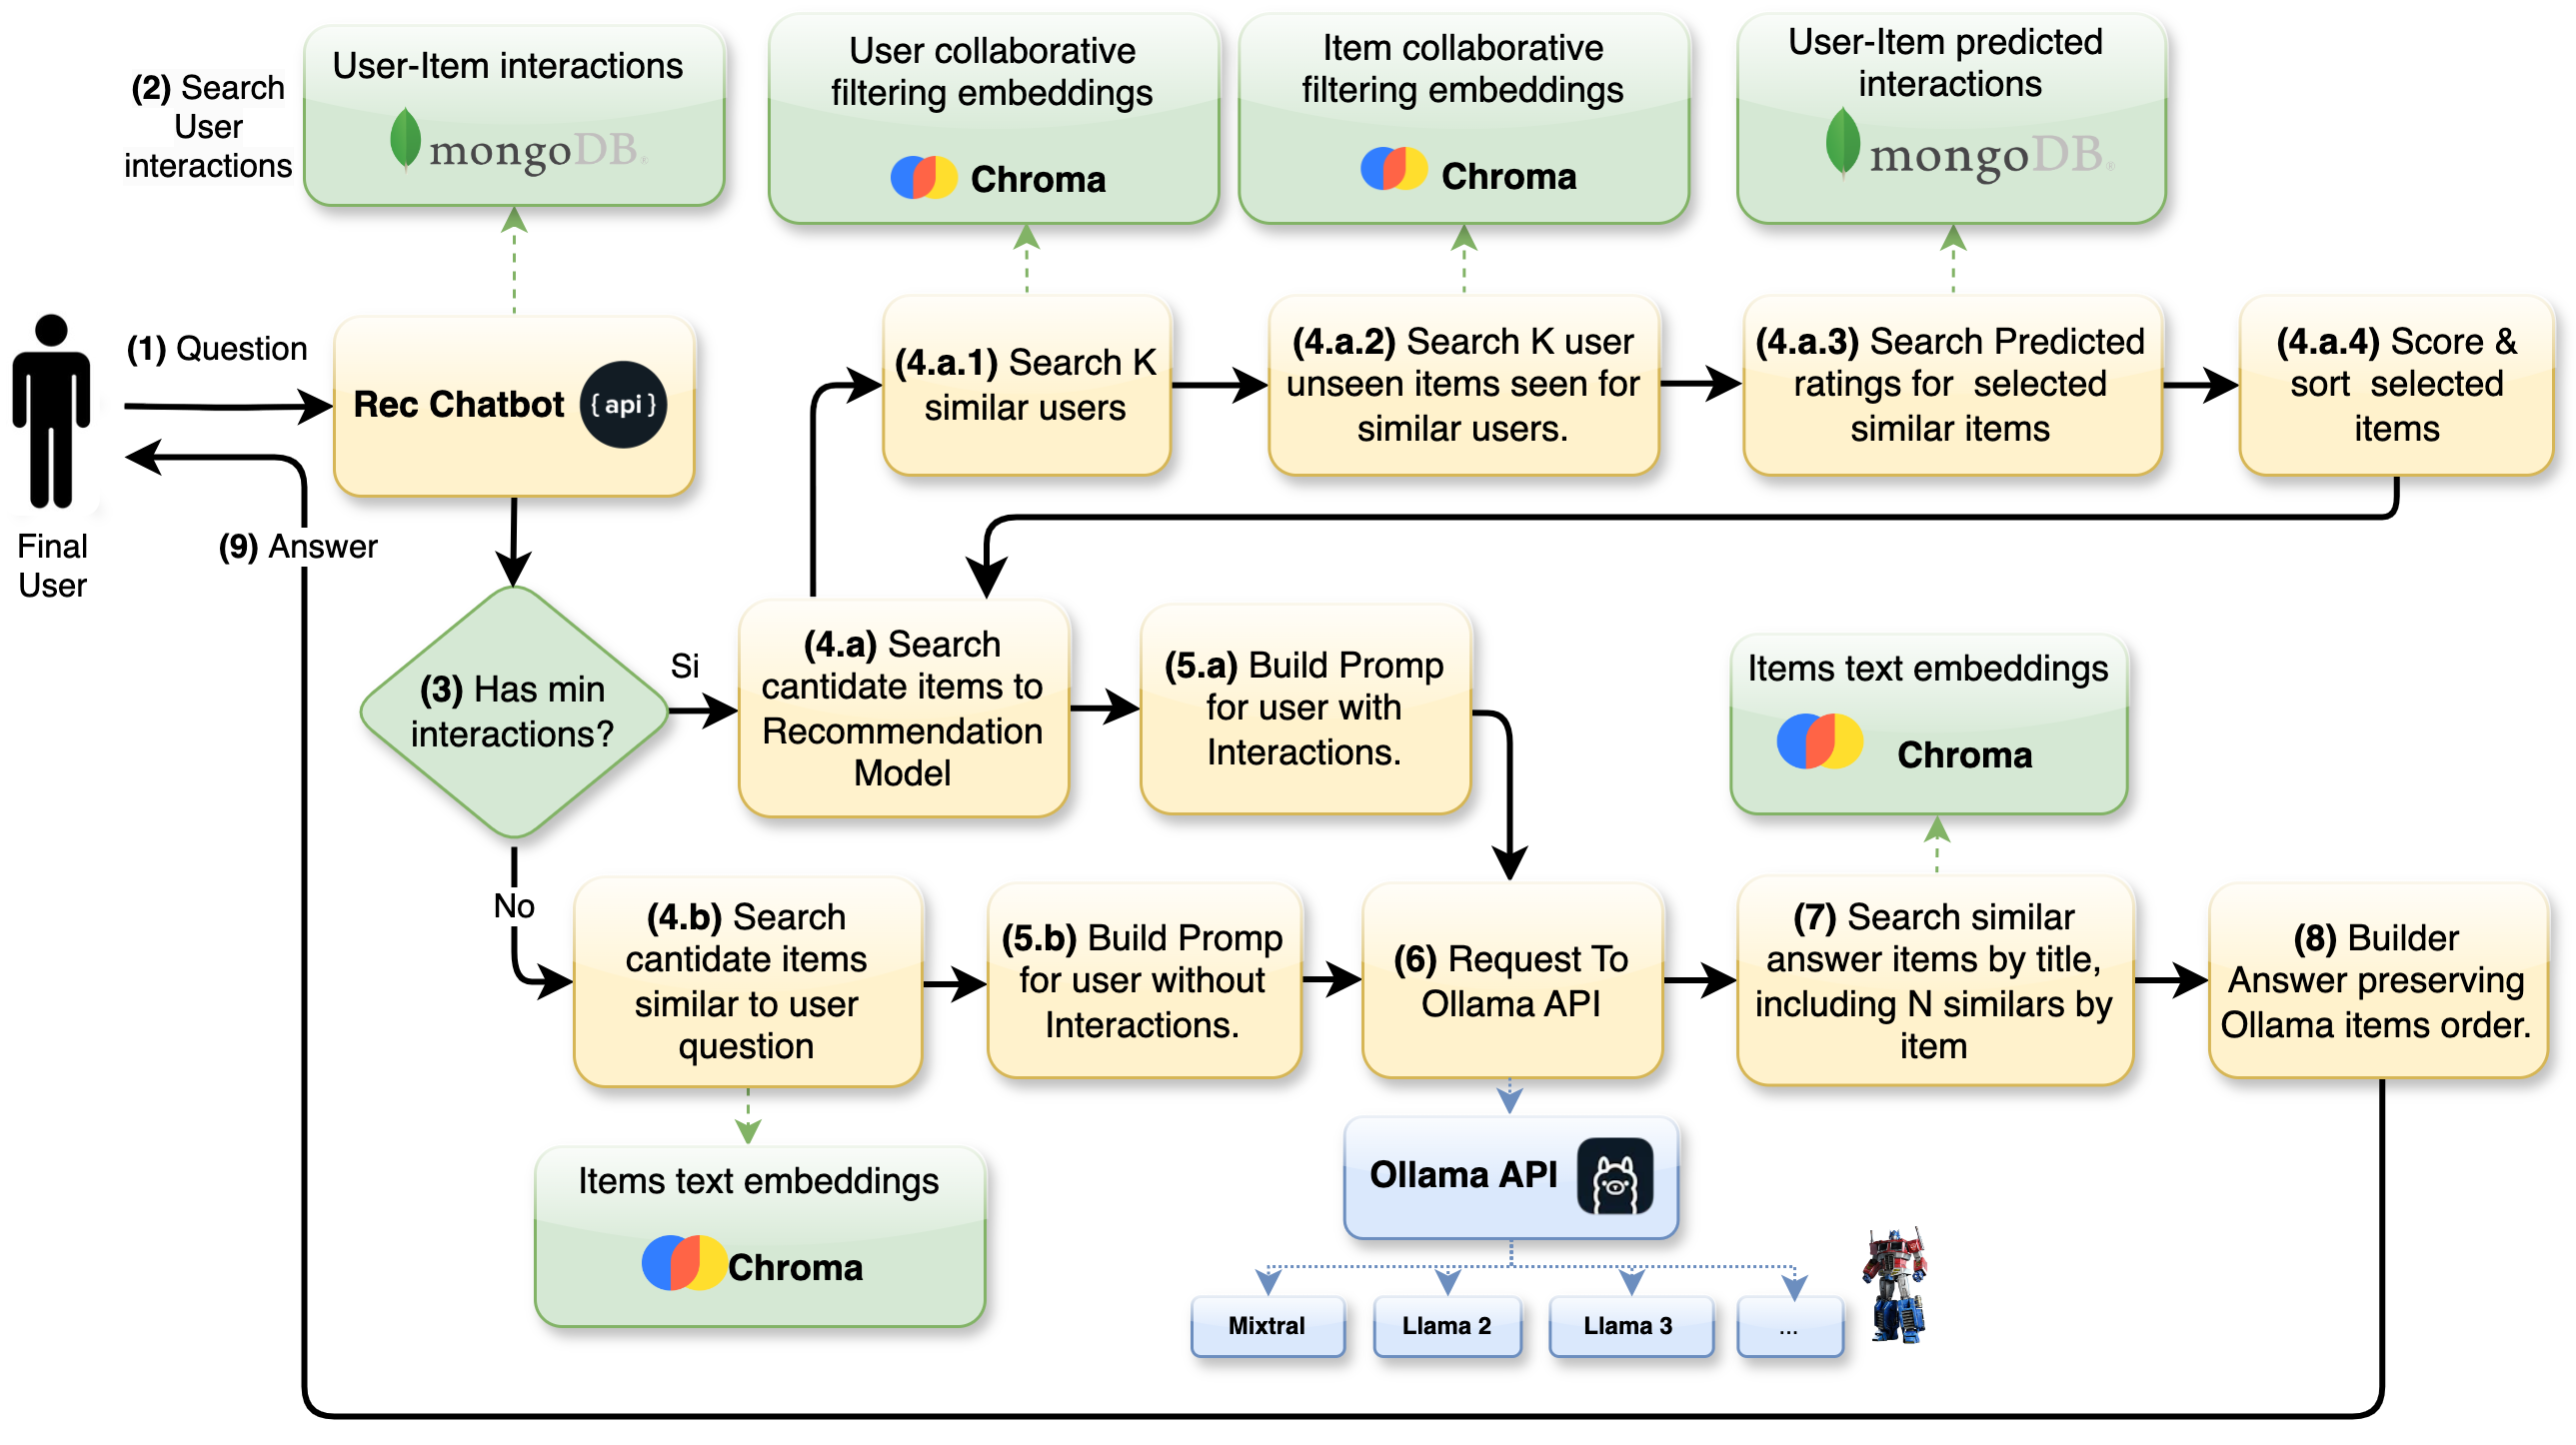
\includegraphics[width=12.5cm]{./images/inference.flow.png}
	\caption{Flujo de inferencia: Este flujo especifica detalladamente todos los pasos secuenciales que lleva a cabo la \textit{API Rec Chatbot} para resolver una recomendación planteada por un usuario utilizando lenguaje natural. Cada etapa en este proceso es crucial para garantizar que la respuesta proporcionada sea adecuada y esté alineada con las necesidades del usuario.}
\end{figure}


Antes de comenzar, aclaramos que al referirnos al usuario final hablamos de aquel que interactúa con una aplicación, ya sea móvil o de escritorio. En este caso, no contamos con una interfaz gráfica, ya que esto va más allá de los objetivos de este trabajo. Por tanto, el término usuario final se refiere a quienes podrían usar una aplicación móvil o de escritorio que consume o integre la \textit{API Rec Chatbot} como parte de su funcionalidad. También existen usuarios más avanzados que interactúan con la \textit{API} a través de un cliente \textit{HTTP}, como \textit{curl}, \textit{Postman} o \textit{Insomnia}. Estos últimos son usuarios con conocimientos sobre cómo interactuar directamente con una \textit{API REST}. En este trabajo, se decidió interactuar directamente con la \textit{API} para simplificar el desarrollo.

Aclarado esto, e comenzara a explicar el flujo de inferencia.


\section{Solicitud de recomendaciones}

Al comienzo del proceso (Paso \textit{1} de la figura \ref{fig:inference-flow}), el usuario tiene la opción de utilizar una aplicación móvil, una aplicación de escritorio o incluso acceder directamente a través de un cliente http. Mediante cualquiera de estos métodos, el usuario puede formular una pregunta en lenguaje natural relacionada con algún contenido que desea visualizar. En este caso específico, se trata de una película, pero también puede referirse a contenido sobre un género particular, una saga específica, o una historia que cuente con cierto tipo de trama, ya sea de acción, drama, comedia, terror, entre otros. Así, el usuario busca obtener información detallada que le ayude a decidir qué ver o comprender mejor el material que le interesa.

\section{Consulta de interacciones del usuario}

En el paso \textit{2} de la figura \ref{fig:inference-flow}, se llevan a cabo la consulta de las interacciones del usuario que formuló la pregunta, accediendo a la base de datos \textit{MongoDB}. Para identificar de manera única al usuario en cuestión, se utiliza su\textit{email} como identificador exclusivo, lo que permite obtener información detallada sobre sus interacciones previas.


\section{¿El usuario realizó el mínimo de interacciones?}

En el paso \textit{2} de la figura \ref{fig:inference-flow}, se cuenta el número de interacciones previas del usuario con la aplicación. Si alcanza el mínimo requerido, se pueden iniciar recomendaciones personalizadas; de lo contrario, se utilizará un esquema de recomendación que puede sugerir contenido sin conocimiento profundo del usuario, ya que no conoce su comportamiento al momento de calificar contenido. Es importante aclarar que las interacciones se refieren a las calificaciones que el usuario otorga a los contenidos. Cada vez que el usuario puntúa una película (por ejemplo, con 5 estrellas), el servicio registra esta interacción y la utiliza para entrenar un modelo de recomendación que personaliza el contenido. Para lograr esto, es necesario contar con un mínimo de interacciones del usuario, lo cual mejora la precisión de las recomendaciones. Este mínimo es un hyper-parámetro más del modelo ensamble o servicio desarrollado. Este paso permite manejar el problema de arranque en frió(\textit{Cold Start}) que sufren los sistemas de recomendación basados en filtros colaborativos. Esto refiere a que estos sistemas de recomendación no pueden entrenarse sin un número mínimo de puntuaciones del usuario. Cuando no se cuenta con esta información es necesario utilizar otros sistemas de recomendación que permitan sugerir contenido hasta que el usuario llegue a este numero mínimo de puntuaciones o calificaciones.

\section{El usuario no cumple con el número mínimo de interacciones}

Cuando el usuario no cumpla con el número mínimo de interacciones (Paso \textit{4.b} de la figura \ref{fig:inference-flow}), se toma su consulta en lenguaje natural y se lleva a cabo la generación de un \textit{Sentence Embedding}, es decir se genera un vector de números que representa al texto de la consulta del usuario. A continuación, con la consulta del usuario ya codificada como un \textit{embedding}, se procede a buscar los \textit{embeddings} más cercanos en la base de datos \textit{ChromaDb}. Este motor de base de datos presenta algunas similitudes con el motor de base de datos \textit{MongoDb}, ya que ambos sistemas organizan los datos en colecciones de documentos. Para proseguir, se realiza la búsqueda dentro de una colección particular llamada \textit{items\_content}, esta colección alberga los \textit{embeddings} que corresponden a todas películas disponibles. Es fundamental aclarar que los \textit{embeddings} se generan a partir de información relativa al título de la película, la sinopsis que la describe y también la lista de géneros cinematográficos a los que pertenece. Estos \textit{embeddings} son producidos mediante modelos de tipo \textit{transformer}; en este caso particular se utiliza el modelo \textit{all-mpnet-base-v2}. Es relevante destacar que estos modelos han sido pre-entrenados específicamente para realizar la tarea de \textit{clustering}, y es importante tener en cuenta que no todos los modelos de lenguaje ofrecen buenos resultados para esta tarea, a menos que hayan sido entrenados específicamente con este propósito.

\section{Construir \textit{prompt} para consulta al modelo de lenguaje}

Después de generar una lista de items similares a la consulta del usuario en el paso anterior, es crucial en este punto (Paso \textit{5.b} de la figura \ref{fig:inference-flow}) ordenar estos items según un \textit{score} específico para identificar los más relevantes para el usuario. Luego, se seleccionarán los primeros n items de esta lista ordenada. Para esta tarea, se pueden usar diversos métodos, ya sean basados en contenido o en filtros colaborativos. Sin embargo, dado que no hay interacciones previas del usuario, se optó por un enfoque basado exclusivamente en el contenido disponible.

Este enfoque es, en cierto modo, poco convencional, ya que inicia con la aplicación de técnicas de \textit{clustering} para identificar contenido que es similar a la consulta realizada, lo cual nos ayuda a reducir el espacio de búsqueda y a centrar nuestra atención en las opciones más relevantes. Después de haber agrupado el contenido similar, se recurre a un modelo de lenguaje grande que tiene la tarea de ordenar los items que se consideran más cercanos a las preferencias del usuario en función de los datos disponibles. Para que el modelo pueda cumplir con esta función de manera efectiva, es necesario crear un \textit{prompt} que contenga información sobre el usuario conocida previamente a su consulta, así como una lista de items candidatos que ya fueron identificados en el paso anterior (Paso \textit{4.b} de la figura \ref{fig:inference-flow}).

Entonces, se le solicita a un modelo de lenguaje grande que realice la tarea de ordenar los items en función de las preferencias del usuario. Es importante resaltar que durante el proceso de experimentación se probaron múltiples tipos de \textit{prompts} con el objetivo de encontrar la estrategia más efectiva. Sin embargo, se observó que los modelos locales mostraron una menor precisión al intentar seguir instrucciones complejas proporcionadas en estos \textit{prompts}. Esta situación llevó a tomar la decisión de utilizar \textit{prompts} más simples, lo cual resultó en una mejora notable en la coherencia y rendimiento del modelo de lenguaje grande al momento de realizar el ordenamiento solicitado.
\vfill

\subsection{\textit{Prompt} para usuarios que no cumple el mínimo de interacciones}

A continuación se puede apreciar la plantilla del \textit{prompt} para tener un idea de como se estructura:

\begin{minted}
[
frame=lines,
framesep=2mm,
baselinestretch=1.2,
bgcolor=LightGray,
fontsize=\footnotesize,
linenos
]
{python}
PROMPT_LOW_INTERACTIONS = """
{user_profile}
{user_history}
{request}
{candidates}

Recommend {limit} movies from candidate movies list, based on 'question', 'user profile'
and 'seen movies'. Return only a list of recommendations with next format:

Number. Title (release year): Synopsis.

Response only has specified content and must have all specified items.
"""
\end{minted}

Para comenzar este es un fragmento de código fuente en lenguaje \textit{Python}. Este código fuente define el \textit{template} o plantilla utilizada para construir dinámicamente el \textit{prompt} para usuarios que no tienen una cantidad mínima de interacciones. Cabe aclarar que existe un \textit{prompt} para cada tipo de usuario: Aquellos que no cumplen con el número mínimo de interacciones y aquellos si lo hacen.

Este \textit{prompt} esta compuesto principalmente por 5 secciones, definidas por un texto dinámico que se reemplaza en cada variable especificada entre corchetes.
\vfill
\subsection{Perfil del usuario}

La variable \textit{user\_profile} contiene el perfil de usuario. Antes que nada se debe registrar el perfil del usuario, sin este no es posible comenzar a realizar consultas a la \textit{API Rec Chatbot}. A contención se puede puede apreciar una solicitud de alta de un perfil de usuario a \textit{API Rec Chatbot}:

\begin{minted}
[
frame=lines,
framesep=2mm,
baselinestretch=1.2,
bgcolor=LightGray,
fontsize=\footnotesize,
linenos
]
{bash}
curl --location 'http://nonosoft.ddns.net:8080/api/v1/profiles' \
--header 'Content-Type: application/json' \
--data-raw '{
 "name"    : "Adrian",
 "email"   : "adrianmarino@gmail.com",
 "metadata": {
   "studies"      : "Engineering",
    "age"         : 42,
    "genre"       : "Male",
    "nationality" : "Argentina",
    "work"        : "Software Engineer",
    "content_preferences": {
        "release": { "from" : "1970" },
        "genres" : [ "thiller", "suspense", "science fiction", "love", "comedy" ]
    }
 }
}'
\end{minted}

Mediante el comando \textit{curl} se realiza una solicito POST para dar de alta el usuario en \textit{API Rec Chatbot}, donde el \textit{request body} contiene los siguientes datos:

\begin{itemize}
	\item Nombre del usuario.
	\item \textit{Email} del usuario: Este es utilizado como identificador único del mismo en el sistema.
	\item Edad, género, nacionalidad y una breve descripción laboral del mismo.
	\item En la sección \textit{content\_preferences} se puede establecer el año mínimo de lanzamiento de una película (\textit{release\_from}), determinando así la antigüedad a partir de la cual se prefieren recomendaciones. Además se puede definir una lista de géneros preferidos en la propiedad \textit{genres}).
\end{itemize}

Con esta información se puede generar el texto que luego se reemplazara en la variable \textit{user\_profile} en el \textit{prompt} principal.

\subsection{Historial de comportamiento del usuario}

La variable \textit{user\_history} presenta una lista detallada de los ítems que han sido calificados por el usuario junto a su calificación. Esto se refiere específicamente a aquellos elementos que el usuario ha llegado a conocer y ha evaluado en función de su experiencia personal. Los ítems están organizados de acuerdo con el \textit{timestamp} de calificación, lo que significa que se presentan en un orden ascendente, comenzando desde el ítem más antiguo que fue calificado hasta llegar al más reciente. Esta disposición permite al lector observar la evolución de las calificaciones a lo largo del tiempo, ofreciendo una perspectiva clara sobre cómo han cambiado las opiniones del usuario sobre cada uno de los ítems evaluados.

\subsection{Solicitud del usuario}

La variable \textit{request} contiene la solicitud del usuario en lenguaje natural. Ejemplo de esas podrían ser:

\begin{itemize}
	\item Quisiera ver una película de Pixar. Cuales me recomendarías?
	\item Quiero ver una película de suspenso ambientada en un futuro disto-pico.
\end{itemize}
\subsection{Items candidatos}

La variable \textit{candidates} contiene la lista de items candidatos resuelta en el paso \textit{4.b} ordenadas por su similitud con la variable \textit{request}.

\subsection{Instrucciones y formato de la respuesta}


Finalmente se especifica las instrucciones que debe seguir el modelo de lenguaje:

\begin{itemize}
	\item Debe seleccionar película a recomendar de la lista de items candidatos.
	\item Para realizar la recomendación, el \textit{LLM} debe basarse en la solicitud del usuario, los datos referentes a su perfil y las películas que ya ha calificado. Con este paso se intenta que el modelo de lenguaje realiza una selecciones los títulos candidatos que mejor correlaciones con esta información.
	\item Se define explícitamente el formato de la respuesta, que consiste en una lista ordenada por un índice numérico que indica relevancia con el título, año de estreno y una breve sinopsis. Debido a la limitada capacidad de comprensión de las instrucciones, se optó por este formato óptimo. Aunque el formato más adecuado habría sido una lista de identificadores, el modelo a menudo no seguía estas indicaciones y devolvía una lista en el formato establecido, lo que aumentó la probabilidad de que el modelo lo respetara.
	\item Finalmente, se enfatiza al modelo de lenguaje la importancia de respetar el ítem de la lista de candidatos, ya que estos modelos tienden a incluir títulos que no son candidatos, nuevamente debido a su baja capacidad para seguir instrucciones.
\end{itemize}

\section{Consulta a modelo de lenguaje}

En el paso 6 de la figura \ref{fig:inference-flow}, se lleva a cabo una solicitud \textit{http} a la \textit{API REST de Ollama}. Durante este paso, los usuarios tienen la opción de seleccionar la distribución del modelo de lenguaje que pueden utilizar. Esta selección es significativa, ya que cada distribución presenta diferentes hiperparámetros, así como variaciones en su tamaño e implementación, lo que puede influir en el rendimiento del modelo general que define \textit{API Rec Chatbot}. Se llevaron a cabo pruebas exhaustivas con varios modelos, y entre ellos, \text{Llama2} y \text{Llama3} demostraron ser los que proporcionan resultados mas coherentes y mas estables , destacándose en comparación con otras alternativas evaluadas.

\section{Búsqueda de items similares en base de datos \textit{ChromaDb} y construcción de respuesta final}

En el paso 7 y 8 de la figura \ref{fig:inference-flow}, se toma la respuesta del \textit{LLM} mencionado anteriormente. Esta respuesta es una lista ordenada de ítems, pero no se puede co-relacionar directamente con los ítems en la base de datos \textit{MongoDb} porque no se proporciona un identificador de ítem. Para resolver esto, se buscan títulos por proximidad en la base de datos \textit{ChromaDb}. Cada título se codifica en un \textit{Sentence embedding} y se busca en la base de datos, generando una lista de N ítems para cada título de la respuesta original. Esto también permite recomendaciones por contenido al ofrecer ítems similares, enriqueciendo la respuesta cuando el modelo de lenguaje no es coherente o tiene menos ítems de los especificados. Este es un hiperparámetro que define cuántos ítems seleccionar. En la evaluación del modelo, se tomó solo un ítem similar, el más cercano a cada ítem de la respuesta original. Es importante señalar que el ítem seleccionado podría no ser el original, sino uno parecido. Esto se relaciona con el problema mencionado anteriormente, donde el modelo podría omitir instrucciones y devolver ítems que no estén en la lista de candidatos ni en la base de datos de \textit{API Rec Chatbot}.

En resumen, este paso transforma la respuesta del \textit{LLM} en una lista de ítems de las bases de datos de la \textit{API Rec Chatbot}. Esta transformación es no determinista, ya que no siempre se obtienen el mismo número de ítems ni los mismos ítems, aunque sucede así la mayoría de las veces. Todo esto sucede dado que los modelos de lenguaje no puede cumplir al pie de la letra con las instrucciones que le son dadas.

Finalmente, se consulta en la base de datos \textit{MongoDB} los documentos correspondientes a cada ítem de la lista resultante. Se agrega el título, la \textit{URL} de su póster (imagen) y se mantiene la descripción generada por el \textit{LLM}, que es más resumida que la sinopsis original. También se toman los géneros del documento y se genera una lista de \textit{URL\'s} que permite al usuario votar por los ítems recomendados. La lista de ítems se devuelve ordenada al usuario, quien puede votar por cada uno de ellos si lo desea. Estas votaciones representan la interacción del usuario con el sistema. Las votaciones se almacenan en la base de datos \textit{MongoDB} en la colección \textit{interactions}, donde cada documento contiene el identificador del usuario, el identificador del ítem, la votación en sí, y la fecha y hora de la votación. Posteriormente, estas interacciones serán consultadas por un proceso que entrena un modelo de recomendación basado en filtrado colaborativo, el cual se utilizará cuando el usuario alcance un número mínimo de interacciones. Esto se desarrollará mejor en los siguientes apartados, donde se detallará el perfil para usuarios con interacciones.
\vfill

\section{Usuarios de cumplen con el mínimo de interacciones}

Hasta ahora, se ha hablado sobre el flujo para tratar a usuarios con pocas interacciones. ¿Qué sucede si ya tenemos un usuario que cumple con el mínimo? Primero, deberíamos contar con un modelo de filtros colaborativos entrenado que incluya a este usuario y sus interacciones hasta ese momento. Esto nos permite utilizar no solo el modelo de lenguaje seleccionado para elegir y ordenas los ítems candidatos, sino también el modelo de filtros colaborativos.
Antes de comenzar, a describir el flujo se debe aclarar que el paso \textit{4.a} en la figura \ref{fig:inference-flow} es igual al paso \textit{4.b}, luego los pasos que si se diferencian serian \textit{4.a.1} en adelante y el \textit{5.a}.
por otro lado, es importante entender que se seleccionaron modelos de filtros colaborativos analizados en el trabajo de especialización previo \cite{src}. Entre ellos, se pueden utilizar aquellos que, tras su entrenamiento, no solo generan un modelo para predecir calificaciones a partir del ID de usuario e ítem, sino que también producen dos colecciones de \textit{embeddings}, una para usuarios y otra para ítems. A medida que los modelos se entrenan, identifican correlaciones entre los usuarios y entre los ítems, lo que se refleja en el ajuste de sus \textit{embeddings} en cada iteración de entrenamiento. Esto permite no solo predecir calificaciones, sino también encontrar usuarios e ítems similares. En este trabajo de hará uso de estas capacidades al momento de la inferencia.

Para los pasas \textit{4.a.1} y \textit{4.a.2} de la figura \ref{fig:inference-flow} es necesario consultar dos colecciones extra de \textit{embeddings}:

\begin{itemize}
	\item \textbf{\textit{items\_cf}}: Contiene los \textit{embeddings} de todos los items del sistema. Estos \textit{embeddings} son generados a partir de entrenamiento del modelo \textit{DeepFM}~\cite{dfmpaper, didldfm}. Este modelo aprende dos \textit{embeddings} de usuarios e items en su entrenamiento.
	\item \textbf{\textit{users\_cf}}: Contiene los \textit{embeddings} de todos los usuarios del sistema aprendidos en el entrenamiento del modelo \textit{DeepFM}~\cite{dfmpaper, didldfm}.
\end{itemize}

Cada colección de \textit{embeddings} contiene metadatos que incluye el identificador único de cada entidad, ya sean usuarios o ítems, lo que facilita la búsqueda de entidades que sean similares o cercanas. A partir del identificador del usuario actual, se procede a buscar otros usuarios que sean similares, lo cual es definido por el hiperparámetro \textit{k\_sim\_users}. Este proceso es crucial para encontrar recomendaciones personalizadas. Una vez obtenidos los usuarios similares, se lleva a cabo la selección de hasta \textit{max\_items\_by\_user} ítems que hayan sido vistos por cada uno de esos usuarios similares.

Durante esta selección, también se aplica dos filtro adicionales:

\begin{itemize}
	\item \textbf{Items con puntuación mínima}: Es la puntuación mínima que debe cumplir cada ítem, la cual es establecida por el hiperparámetro \textit{min\_rating\_by\_user}. Por defecto, esta puntuación mínima se encuentra en \textit{3.5} puntos, asegurando que solo aquellos ítems que han recibido una valoración aceptable sean considerados en la recomendación, lo que ayuda a mejorar la calidad de las sugerencias para el usuario actual.
	\item \textbf{Item no vistos}: Además se filtran los items no vistos por el usuario actual, definido por el hiperparámetro \textit{not\_seen}.
\end{itemize}

Cabe aclarar que la selección de items se realiza al azar y esta definida por el hiperparámetro \textit{random\_selection\_items\_by\_user}, cuyo valor predeterminado es \textit{0.5}. Es decir, el \textit{50\%} de las veces se selecciona un ítem al iterar la lista de items de cada usuario que cumple con la restricción anteriormente definidas.

A este punto resta aplicar algún tipo de ordenamiento a la lista de items candidatos, a la cual finalmente se le aplicara un segundo ordenamiento mediante el modelo de lenguaje (Paso 5.a de la figura \ref{fig:inference-flow} en adelante).

Para ordenar los candidatos se probaron distintos enfoques.

\textbf{\textit{pred\_user\_rating}}: Se ordena según las calificaciones predichas por el modelo de filtros colaborativos(\textit{DeepFM}~\cite{dfmpaper, didldfm}), que indica la calificación que el modelo estima que el usuario otorgaría al ítem. Esta es la medida mas personalizada pero sola no es muy efectiva.

\textbf{\textit{user\_item\_sim}}: Representa la similitud entre el usuario que solicita la recomendación y el usuario que calificó el ítem seleccionado. Esto puede causar que ítems con el mismo \textit{score} se repitan, especialmente en el caso de \textit{fun users} que suelen calificar muchas películas de un mismo género, lo que puede hacer que sus ítems aparezcan primero. Es importante tener en cuenta que los ítems pueden repetirse entre diferentes usuarios, lo cual es normal. Por ello, se debe elegir una estrategia para aplicar una media o mediana al \textit{score} en casos de repetición. Esto influye en cierta medida en la personalización del orden, por lo que es preferible adoptar las siguientes estrategias.

\textbf{\textit{user\_sim\_weighted\_rating\_score}}: Se asigna un \textit{score} a cada ítem según la similitud entre el usuario que solicita la recomendación y el que lo calificó, ponderado por la calificación media de los usuarios más cercanos. Esta estrategia soluciona el problema de tener bloques de ítems por usuario cercano, pero pierde personalización al utilizar la calificación media en lugar de la que otorgaría el usuario que realizó la consulta. Esto se aborda en la siguiente estrategia.

\begin{equation}
	User Sim Weighted By Rating = User Sim * \frac{Item User Preducted Rating}{Max Items User Predicted Rating}
\end{equation}

\textbf{\textit{user\_sim\_weighted\_pred\_rating\_score}}: Es similar al \textit{score} anterior, pero más personalizado, ya que se ajusta según la calificación que se estima que el usuario otorgaría al ítem. La métrica anterior utiliza el promedio o mediana del \textit{rating} general del ítem para usuarios cercanos, proporcionando cierto grado de personalización, pero aquí se pondera por la calificación específica predicha para el usuario que solicitó la recomendación, lo que la hace más personalizada.

\begin{align}
	User Sim Weighted By Pred Rating = User Sim * \frac{Item User Pred Rating}{Max Items User Pred Rating}
\end{align}

Para continuar con nuestro flujo, solo queda aplicar alguno de los métodos de \textit{scoring} a los ítems candidatos definido mas arriba. A diferencia del flujo para usuarios sin interacciones, donde la similitud de los ítems con la consulta del usuario define el orden de los ítems candidatos, aquí se utiliza un \textit{score} basado en el aprendizaje de un modelo de filtrado colaborativo. Esta es la sutil diferencia. Posteriormente, el modelo de lenguaje ajustará el ordenamiento en un segundo filtro. Así, obtenemos un \textit{score} personalizado que considera las correlaciones en el comportamiento del usuario con otros usuarios, así como la relación de su historia y perfil con los ítems candidatos.

\vfill
\chapter{Flujo de entrenamiento de \textit{Rec Chatbot API}}

En la sección anterior se presentó el flujo de inferencia del modelo de recomendación \textit{Rec Chatbot API}. En ese flujo, contábamos con \textit{embeddings} disponibles en una base de datos lista para utilizar. También disponíamos de modelos pre-entrenados. Sin embargo, ¿cómo se generan estas herramientas a partir de los datos que ingresan \textit{Rec Chatbot API}? En este apartado, explicaremos el proceso de entrenamiento, que se encargará de generar y mantener actualizados estos modelos y \textit{embeddings}, basándose en las actualizaciones de información en la base de datos de \textit{Rec Chatbot API}, incluyendo altas y bajas de perfiles de usuarios y sus calificaciones. Para comenzar, se desarrollaron dos procesos o flujos que permiten esto:

\begin{itemize}
	\item El primer flujo realiza el entrenamiento de un modelo de recomendación basado en filtros colaborativos, que puede ser sustituido por cualquier modelo que prediga calificaciones entre 0 y 5 y que ajuste vectores de \textit{embedding} para aprender características entre usuarios e ítems. En este trabajo, se eligió un modelo con arquitectura \textit{DeepFM}~\cite{dfmpaper, didldfm}, aunque también se podrían emplear otros como \textit{GMF}, \textit{Biased-GMF} o \textit{NN-FM}. Para más detalles, consulte \cite{src}, donde se explican estos modelos en detalle y se comparan sus resultados.
	\item El segundo flujo se encarga de actualizar los \textit{embeddings} necesarios para la búsqueda de ítems similares o mas cercanos a la consulta del usuario (Técnica \textit{RAG}(\textit{Retrieval Augmented Generation} o Generación Aumentada por Recuperación) ~\cite{rag}).
\end{itemize}


\section{Flujo de Entrenamiento}

Para gestionar de manera efectiva y ejecutar este flujo de trabajo, se eligió la herramienta conocida como \textit{Apache Airflow}. Esta plataforma es altamente eficiente y permite programar, ejecutar y monitorizar tareas complejas de forma organizada. En \textit{Apache Airflow}, los procesos se definen utilizando estructuras denominadas grafos dirigidos acíclicos \textit{(DAG)}, donde cada uno de los nodos dentro del grafo representa una tarea específica a llevar a cabo. Cabe señalar que estas tareas están diseñadas para ser reutilizadas según se necesite, lo que facilita el mantenimiento de los flujos de trabajo.

En el marco de este proyecto, la utilización de \textit{Apache Airflow} se torna fundamental, ya que garantiza la automatización y orquestación de múltiples procesos importantes que están relacionados directamente con el re entrenamiento de modelos, así como con la gestión de datos necesarios para asegurar un funcionamiento efectivo de \textit{Rec Chatbot API}. Esta herramienta no solo permite llevar a cabo los procesos de manera eficiente, sino que también ofrece una forma clara de visualizar el flujo de trabajo en su totalidad. A continuación, en la figura \ref{fig:training-flow}, se puede apreciar un diagrama de flujo ilustrativo que describe en detalle cada uno de los pasos que componen el proceso de entrenamiento \textit{(DAG)}.

\begin{figure}[H]
	\centering
	\label{fig:training-flow}
	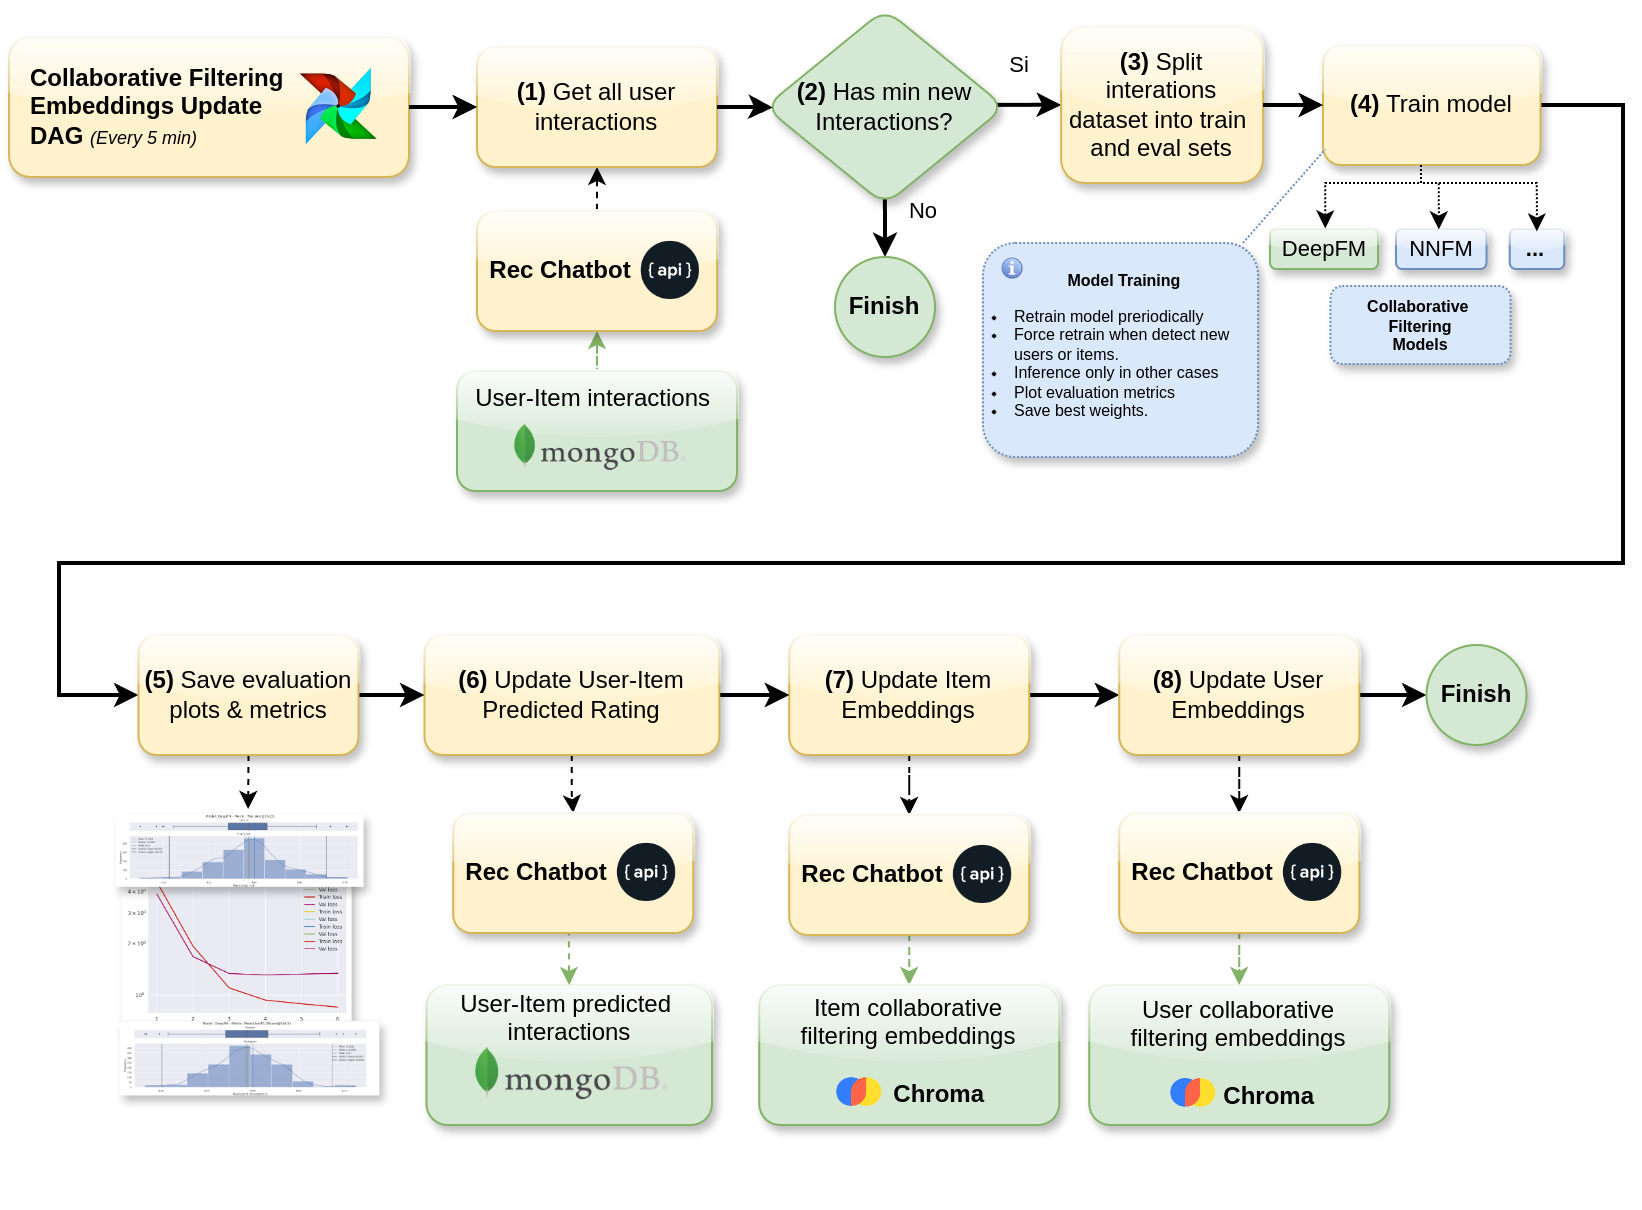
\includegraphics[width=12cm]{./images/training.flow.png}
	\caption{Flujo de entrenamiento: Es un proceso que correr en segundo plano, encargado de entrenar el modelo de filtros colaborativos y actualizar los \textit{embeddings} de usuarios e items.}
\end{figure}


En el paso \textit{1} del flujo de la figura \ref{fig:training-flow}, se solicita a \textit{Rec Chatbot API} las interacciones de los usuarios con los ítems disponibles, representadas como tuplas \textit{(user\_id, item\_id, rating)}. El proceso \textit{DAG} registra el número de interacciones procesadas en ejecuciones anteriores, permitiendo determinar cuántas nuevas interacciones han ocurrido desde la última ejecución. Si la diferencia supera \textit{50} (un valor configurable), se activa el entrenamiento; de lo contrario, se finaliza el \textit{DAG} (Paso \textit{2}). Esta estrategia es útil para gestionar un gran número de usuarios e interacciones en aplicaciones escalables. Cuando el número de usuarios varía poco, se podría evitar el re-entrenamiento completo del modelo, ajustándose solo a las nuevas interacciones. Sin embargo, esto debe manejarse con precaución para evitar el sobre ajuste a las nuevas interacciones y descuidar las anteriores. Dado que en aplicaciones de gran escala es común un aumento constante de perfiles de usuario, esta estrategia puede no ser óptima, siendo más eficiente re-entrenar el modelo completo solo cuando sea necesario. Lo mismo ocurre con los ítems (películas), ya que es habitual que se añadan nuevos ítems y se eliminen otros en plataformas de contenido, lo que requiere re-entrenamiento.


Al llegar al paso \textit{3}, el proceso identifica interacciones nuevas y potencialmente nuevos perfiles de usuario. Dado que la \textit{API Rec Chatbot} es escalable y puede tener millones de usuarios, no es óptimo re-entrenar  el modelo de forma constante ya que se deben economizar recursos. Las instancias de \textit{Apache Airflow} suelen ser ejecutadas en contenedores de \textit{Docker} en en una nube, como \textit{Google Cloud Services}, lo que genera costos dependiendo del \textit{hardware} seleccionado, uso de \textit{CPU}, \textit{GPU}, almacenamiento, etc. Por ello, se debe re-entrenar el modelo lo menos posible, solo lo justo y necesario. Para lograrlo, se implementó una abstracción llamada \textit{ModelLoader} en \textit{Python}, que permite cargar modelos desde un archivo de pesos y prepararlos para la inferencia. \textit{ModelLoader} permite establecer los criterios bajo los cuales se debe re-entrenar el modelo:

\begin{itemize}
	\item El modelo se re-entrena periódicamente, lo que significa que hay un período durante el cual solo se utiliza para inferencia.
	\item Si las nuevas interacciones son de usuarios e items existentes, no se requiere re-entrenamiento, y se espera hasta el siguiente ciclo de re-entrenamiento. Sin embargo, si hay interacciones de nuevos usuarios o items, es necesario forzar el re-entrenar  del modelo, ya que de lo contrario no se podrían realizar inferencias sobre los mismos, dado que el modelo necesita generar \textit{embeddings} para estos usuarios o items necesarios para la inferencia.
\end{itemize}

El \textit{ModelLoader} determina cuándo re-entrenar el modelo. Si decide no re-entrenar, carga el modelo con los pesos del último entrenamiento; de lo contrario, se re-entrena, guarda los mejores pesos y luego carga el modelo para su inferencia. Durante el entrenamiento, \textit{ModelLoader} genera gráficas para monitorear el proceso y verificar el ajuste del modelo, permitiendo ajustes en los hiperparámetros si es necesario. Cada ejecución produce un nuevo conjunto de gráficas para rastrear el historial de entrenamiento (Paso \textit{5}).

En este punto del proceso \textit{DAG}, contamos con un modelo de filtro colaborativo entrenado y listo para la inferencia. En el paso \text{6}, se realiza la inferencia de las calificaciones de ítems para los cuales los usuarios aún no han hecho una valoración. Luego, el \text{DAG} envía una solicitud \text{HTTP} a la \textit{Rec Chatbot API} para guardar estas predicciones, que se utilizarán en el proceso de inferencia del modelo de recomendación de \textit{Rec Chatbot API} para ordenar los ítems recomendados a cada usuario.

Para llevar a cabo los pasos \text{7} y \text{8}, es necesario extraer del modelo de filtros colaborativos dos listas de \text{embeddings}: una correspondiente a los usuarios y otra a los ítems. Se conoce la asignación de cada \text{embedding} a su usuario e ítem asociado. De este modo, se efectúan dos llamadas \text{HTTP} a la \text{API de Rec Chatbot} para persistir las nuevas versiones de los \text{embeddings} de usuarios e ítems generadas durante el entrenamiento del modelo. Posteriormente, estos \text{embeddings} son utilizados por el modelo de recomendación de la \text{Rec Chatbot API} para buscar ítems calificados por usuarios similares y también para encontrar ítems que sean similares a los resultados de una consulta del usuario.


\subsection{Flujo de actualización de búsquedas (Técnica \textit{RAG}(\textit{Retrieval Augmented Generation} o Generación Aumentada por Recuperación))}

Este flujo se ejecuta manualmente y genera \textit{embeddings} para cada ítem, utilizando el título, la sinopsis y los géneros de cada película. Para ello, emplea un modelo conocido como \textit{Sentence Transformers}, que permite crear \textit{embeddings} a partir de oraciones o párrafos. Estos \textit{embeddings} son utilizados posteriormente para identificar los ítems más cercanos a una consulta de usuario.

\begin{figure}[H]
	\centering
	\label{fig:rag-update-flow}
	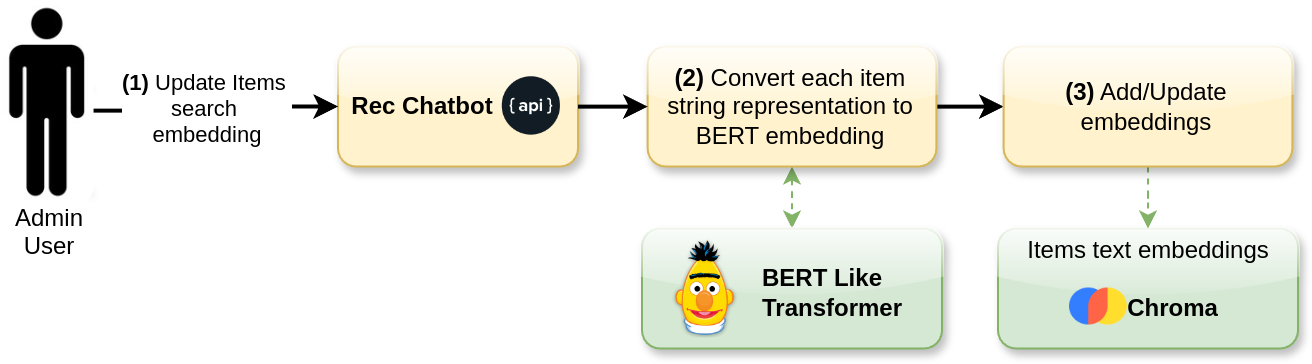
\includegraphics[width=10cm]{./images/rag-embedding-update.png}
	\caption{Flujo de generación y actualización \textit{embeddings} utilizados para la búsqueda de items cercanos a una consulta del usuario (Técnica \textit{RAG}(\textit{Retrieval Augmented Generation} o Generación Aumentada por Recuperación) ~\cite{rag}).}
\end{figure}

\chapter{Modelo interno basado en filtros colaborativos}

En un trabajo previo de especialización \cite{src} de la maestría, se exploraron diversos enfoques para implementar sistemas de recomendación, incluyendo \textit{KNN}. Sin embargo los modelos basados en \textit{KNN} presentan varias limitaciones significativas, siendo el problema de escala uno de los más importantes. El tamaño de los datos a procesar depende casi linealmente de los recursos de memoria, \textit{CPU} y/o \textit{GPU} disponibles. Por lo tanto, al necesitar procesar grandes volúmenes de datos para hacer predicciones, se suelen elegir modelos que aplican algún tipo de reducción de dimensionalidad para construir su representación interna, la cual se utiliza posteriormente para realizar predicciones. Esta representación interna se denomina a menudo "modelo", ya que lo que define el modelo no es el algoritmo en sí, sino el estado interno alcanzado tras el entrenamiento.

\section{Codificación \textit{One-Hot} vs \textit{Embeddings}}

Particularmente en el ámbito de recomendaciones, se cuenta con variables
categóricas de alta dimensionalidad. Para este trabajo, tenemos dos variable
con esta característica: los identificadores secuenciales de usuarios e ítems.
Cuando trabajamos con modelos de \textit{Machine Learning}, particularmente con
redes neuronales, es necesario convertir las variable categóricas en una
representación numérica. El enfoque mas simple o \textit{naive} consiste en
realizar una codificación \textit{one-hot} de la variable categórica, la cual
consta de codificar cada posible valor de la variable como un vector que
contiene tantas posiciones como valores tenga la variable. De esta forma, cada
vector tiene un valor $1$ en la posición que concuerde con el valor
representado y un valor $0$ (cero) en las demás posiciones. Por ejemplo,
suponemos que tenemos la siguiente variable:

\begin{itemize}
	\item Variable Categórica: Estado del Tiempo.
	\item Posibles valores: Nublado, Despegado y Lluvioso.
\end{itemize}

Si codificamos sus valores usando una codificación \textit{one-hot},
obtendremos los siguientes vectores:

\begin{itemize}
	\item $Nublado    = [1, 0, 0]$
	\item $Despegado  = [0, 1, 0]$
	\item $Lluvioso   = [0, 0, 1]$
\end{itemize}

Entonces, el valor \textit{Nublado} se convierte en 3 entradas para una red
neuronal a las cuales se le pasa los numero $1$, $0$ y $0$ respectivamente.
Ahora pensemos en la cantidad de usuarios que tiene \textit{Google} o
\textit{Amazon}. ¿Qué tamaño tendría el vector que representa a un solo
usuario?¿Por qué usar un vector 99\% ralo para representar un valor?¿No hay una
forma mas compacta de realizar esta codificación?

La respuesta corta es sí, en estos casos se utilizan \textit{Embeddings}. ¿Pero
qué son los \textit{Embeddings} y en qué se diferencian de la codificación
\textit{one-hot}?

Un \textit{Embedding} no es mas que una forma de codificar valores de una
variable categórica usando vectores de menor tamaño. Es decir, si tenemos una
variable categórica que tiene 10.000 posible valores, dependiendo del caso,
podríamos elegir un tamaño de 100 posiciones. Este tamaño debe ser elegido de
forma tal que no se produzca pérdida de información. Por esta cuestión, el
tamaño de estos vectores se transforma en un hiperparámetro mas a ajustar al
momento de entrenar los modelos que utilicen esta técnica de codificación.

Otro punto importante que diferencia ambas codificaciones, reside en la
distancia entre vectores. Si tomamos dos vectores con codificación
\textit{one-hot} y los gráficas en un espacio tridimensional o bidimensional,
se aprecia que el ángulo entre estos siempre es el mismo, 90 grados. Supongamos
el caso anterior de la variable Estado del Tiempo, si representamos en el
espacio todos sus valores, podemos ver que la distancia es las misma entre
cualquier par de vectores. Si ahora codificamos la misma variable usando
\textit{Embeddings} esto cambia, ya que los vectores que representan a los
valores Nublado y Lluvioso tiene un ángulo menor a 90 grados. Por otro lado,
ambos vectores están alejados del vector Despejado. De esta forma, un
\textit{Embedding} permite captar mas información, ya que realiza una
clusterización o agrupación de los valores que son mas cercanos en términos de
significado. Los días nublados y lluviosos son muy parecido entre sí y muy
distintos a un dia despejado.

De esta forma los \textit{Embeddings} tiene una doble ganancia sobre la
codificación \textit{One-Hot}: comprimen la información y además captan
información útil para la clusterización o agrupación de sus valores. Algo
interesante a destacar, es que los modelos que entrenan \textit{Embeddings}
captan esta información de forma automática en base a las observaciones usadas
en el entrenamiento, generando estos espacios latentes llamados
\textit{Embeddings}.

\section{Capa o módulo \textit{Embedding}}

En el ámbito del \textit{Deep Learning} o \textit{Machine Learning} se cuenta
con la abstracción de capas (en \textit{frameworks} como \textit{Keras}) o
módulos (en \textit{PyTorch}), las cuales encapsulan el comportamiento esencial
en un conjunto de bloques básicos utilizados para construir cualquier modelo.
Los bloques que permiten que un modelo infiera o construya un
\textit{embedding} durante el entrenamiento, son los bloques \textit{Embedding}
y \textit{EmbeddingBag} en \textit{PyTorch} o simplemente \textit{Embedding} en
\textit{Keras}.

Por un lado, podemos elegir el tamaño de los vectores \textit{embedding}, el
cuál, como ya adelantamos, es un hiperparámetro mas a optimizar. Por otro
lado, debemos definir la cantidad de vectores de \textit{embedding} que debe
contener la capa. Ésta es siempre igual al número total de valores que puede
tomar la variable categórica a codificar.

De esta forma, si deseamos crear una capa o módulo \textit{Embedding} para la
variable categórica Estado del Tiempo, deberíamos crear una capa de tamaño 3,
ya que cuenta con 3 posible valores, con un tamaño de vector menos a 3, ya que
de lo contrario, tendríamos la misma dimensionalidad que tenemos al usa la
codificación \textit{one-hot}, con la diferencia de que una capa
\textit{Embedding} capta la similitud entre los valores de la variable
categórica a diferencia de la codificación \textit{one-hot}.

El modo de funcionamiento de la capa es muy simple. Esta se puede pensar como
una tabla de \textit{Hash}, donde cada clave es un valor de la variable
categórica. Es decir, que tendremos tantas claves como valores pueda tomar la
variable categórica. Estas claves son codificados a números y los valores
asociados a cada clave son vectores \textit{embedding}. Cave aclarar que en
general, estos vectores son inicializados con valores aleatorios. Finalmente,
en la etapa de entrenamiento, el modelo irá ajustando los valores de cada
vector \textit{embedding}.

\clearpage

En la etapa de \textit{forward pass}, se pasa como entrada un valor de la
variable categórica codificado como numérico. Para nuestra variable Estado del
Tiempo podríamos codificar sus valores como sigue:

\begin{itemize}
	\item Nublado $=> 0$
	\item Despegado $=> 1$
	\item Lluvioso $=> 2$
\end{itemize}

Entonces, si pasamos el valor Nublado como entrada a la capa, en realidad
estamos pasando la número o clave \textit{hash} $0$. Luego de esto, la capa
resuelve el vector \textit{embedding} asociado a esa clave y lo devuelve a su
salida.

Finamente, debemos tener en cuenta que el proceso de \textit{back-propagation}
sera el encargado de ir ajustando los valores, también llamados pesos de los
vectores \textit{embedding}, de acuerdo a lo que se requiera en la salida del
modelo durante el proceso de optimización.

\begin{figure}[ht!]
	\centering
	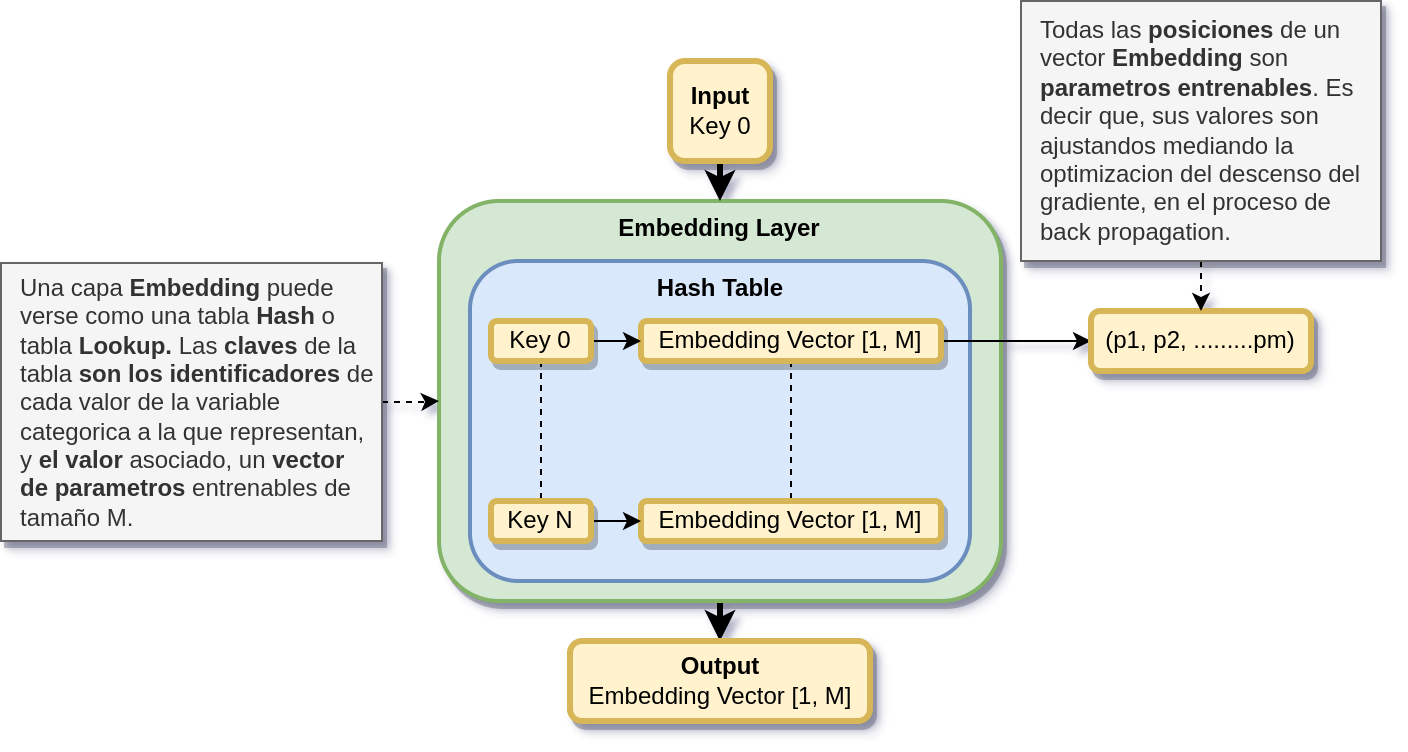
\includegraphics[width=13cm]{./images/Embedding-Layer.png}
	\caption{Esquema de una capa o módulo \textit{Embedding}.}
	\label{fig:embeddingLayer}
\end{figure}

\clearpage



\section{Máquinas de Factorización (\textit{FM})}

Antes de introducir el modelo de máquinas de factorización profundas
(\textit{DeepFM}~\cite{dfmpaper, didldfm}) se comenzara explicando uno de sus componentes mas
importantes: las máquinas de factorización~\cite{didlfm, zhangdive}.

Las máquina de factorización propuestas por \textit{Steffen Rendle} en 2010
~\cite{fm}, son algoritmos supervisados que puede ser utilizados para tareas de
clasificación, regresión y tareas de ranking como sucede en el ámbito de los
sistemas de recomendación. Rápidamente se convirtieron en un método popular
para hacer predicciones y recomendaciones. La máquina de factorización es una
generalización de un modelo lineal y un model de factorización de matrices, mas
aun, recuerdan mucho a un máquina de soporte vectorial \textit{(SVM)} que
utiliza un kernel polinomial.

A continuación, se define el modelo formalmente:

\begin{itemize}
	\item $x\in\mathbb{R}^{d}$ es un vector de características donde cada una de sus
	      componentes representa a una variable del conjunto de datos, siendo $d$
	      la cantidad de variables. En nuestro caso,
	      $x\in\mathbb{R}^{2}$ ya que tenemos dos variables, usuarios e ítems.
	\item $y\in\mathbb{R}$ es la variable \textit{target} o resultado a predecir.
	      Dado el dominio del conjunto de datos seleccionado, seria la
	      calificación del usuario.
\end{itemize}

Luego, podemos definir el modelo para una máquina de factorización de grado $2$
de la siguiente forma:

\begin{equation}
	\hat{y}(x) = \mathbf{w}_0 + \sum_{i=1}^d \mathbf{w}_i x_i + \sum_{i=1}^d\sum_{j=i+1}^d
	\langle\mathbf{v}_i, \mathbf{v}_j\rangle x_i x_j
\end{equation}
\begin{description}
	\item[Donde:]
\end{description}
\begin{itemize}
	\item $d$ es la cantidad de características o variables a utilizar.
	      Para el caso de estudio en este trabajo $d=2$ (usuarios e ítems).
	\item $\mathbf{w}_0 \in \mathbb{R}$ es el \text{bias} o intercepto del modelo.
	\item $\sum_{i=1}^d \mathbf{w}_i x_i$: Esta es la parte lineal del modelo. Aquí,
	      $x_i$ representa el valor del \textit{feature} $i$-ésimo. $\mathbf{w}_i$ es
	      el peso asociado al \textit{feature} $i$-ésimo, que determina la influencia
	      de ese \textit{feature} en la predicción. Multiplicamos el valor de cada
	      \textit{feature} $x_i$ por su peso correspondiente $\mathbf{w}_i$ y sumamos
	      todas estas contribuciones para obtener la parte lineal de la predicción.
	\item $\sum_{i=1}^d\sum_{j=i+1}^d \langle\mathbf{v}_i, \mathbf{v}_j\rangle x_i x_j$:
	      Esta es la parte de factorización del modelo. Donde, $\langle\mathbf{v}_i,
		      \mathbf{v}_j\rangle$ es el producto interno (o producto escalar) entre
	      los vectores $\mathbf{v}_i$ y $\mathbf{v}_j$. Cada vector $\mathbf{v}_i$
	      representa una factor latente o \textit{Embedding} del \textit{feature}
	      $i$-ésimo. Estos vectores capturan interacciones no lineales entre
	      características y se utilizan para modelar relaciones más complejas
	      entre ellas. Similar a la parte lineal, multiplicamos los valores
	      de las características $x_i$ y $x_j$ por el producto interno
	      $\langle\mathbf{v}_i, \mathbf{v}_j\rangle$ y sumamos todas las contribuciones
	      para obtener la parte de factorización de la predicción.

\end{itemize}

En resumen, la expresión completa $\hat{y}(x)$ representa la estimación de la
variable dependiente $\hat{y}$ basada en la entrada $x$, utilizando una
combinación lineal de los pesos de las características y una suma de productos
internos entre los vectores de características latentes para capturar
interacciones no lineales entre las características. Este modelo es comúnmente
utilizado en el campo del aprendizaje automático para problemas de regresión y
clasificación.

De esta forma los dos primeros términos corresponden al modelo de regresión
lineal y el último término es una extensión del modelo de factorización
matricial. Si la variable $i$ representa un ítem y la variable $j$ a un
usuario, el tercer término es el producto escalar entre los vectores
\textit{embedding} de usuario $u$ y ítem $i$. Por otro lado, vale la pena
aclarar que este método también puede generalizar en órdenes superiores al
grado 2, sin embargo, la estabilidad numérica podría disminuí la generalización
del método.

Al aplicar un método de optimización con las máquinas de factorización, como
puede ser el método del gradiente descendente, se puede llegar fácilmente a una
complejidad del orden $\mathcal{O}(kd^2)$, ya que se deben calcular todas las
interacciones de a pares. Para resolver este problema de \textit{performance},
podemos reorganizar el tercer término del método, Esto reduce en gran medida el
costo de cálculo, llevándolo a una complejidad de tiempo de orden lineal
$\mathcal{O}(kd)$. A continuación se describen los pasos para bajar el nivel de
complejidad del método:

\begin{equation}
	\begin{split}
		 & =\sum_{i=1}^d \sum_{j=i+1}^d \langle\mathbf{v}_i, \mathbf{v}_j\rangle x_i x_j                                                                                                       \\
		 & = \frac{1}{2} \sum_{i=1}^d \sum_{j=1}^d\langle\mathbf{v}_i, \mathbf{v}_j\rangle x_i x_j - \frac{1}{2}\sum_{i=1}^d \langle\mathbf{v}_i, \mathbf{v}_i\rangle x_i x_i                  \\
		 & = \frac{1}{2} \big (\sum_{i=1}^d \sum_{j=1}^d \sum_{l=1}^k\mathbf{v}_{i, l} \mathbf{v}_{j, l} x_i x_j - \sum_{i=1}^d \sum_{l=1}^k \mathbf{v}_{i, l} \mathbf{v}_{i, l} x_i x_i \big) \\
		 & =  \frac{1}{2} \sum_{l=1}^k \big ((\sum_{i=1}^d \mathbf{v}_{i, l} x_i) (\sum_{j=1}^d \mathbf{v}_{j, l}x_j) - \sum_{i=1}^d \mathbf{v}_{i, l}^2 x_i^2 \big )                          \\
		 & = \frac{1}{2} \sum_{l=1}^k \big ((\sum_{i=1}^d \mathbf{v}_{i, l} x_i)^2 - \sum_{i=1}^d \mathbf{v}_{i, l}^2 x_i^2)
	\end{split}
\end{equation}

Con esta re-formulación del último termino, la complejidad del método se reduce
considerablemente. Además, para las variables ralas, solo se deben computar los
valores distintos de cero, para que la complejidad general sea lineal.
Finalmente, la expresión del método aplicando esta re-formulación queda como
sigue:

\begin{equation}
	\hat{y}(x) = \mathbf{w}_0 + \sum_{i=1}^d \mathbf{w}_i x_i + \frac{1}{2} \sum_{l=1}^k \big ((\sum_{i=1}^d \mathbf{v}_{i, l} x_i)^2 - \sum_{i=1}^d \mathbf{v}_{i, l}^2 x_i^2)
\end{equation}

\clearpage

\section{Máquinas de factorización profundas (\textit{DeepFM})}

Hasta aquí, a grandes rasgos, todos los modelos expuestos tratan de captar el
comportamiento de las interacciones o correlación usuario-ítems, ya sean
implícitas o explicitas. A pesar de este gran progreso, los métodos expuestos
anteriormente (exceptuando las máquinas de factorización) parecen tener un
fuerte sesgo al predecir las interacciones o correlaciones de bajo y alto
orden, requiriendo en algunos casos realizar ingeniería de características
para disminuir estos sesgos.

El modelo de máquinas de factorización profundas
(\textit{DeepFM})~\cite{dfmpaper, didldfm} o maquina de factorización basada en
\textit{Deep Learning}, mejora el aprendizaje de las interacciones o
correlaciones de bajo y alto orden. Este modelo combina máquinas de
factorización y \textit{Deep Learning} en una nueva arquitectura de red
neuronal, la cual captura estas correlaciones. Por otro lado, es una evolución
del modelo \textit{Wide and Deep}~\cite{wideanddeeppaper} de \textit{Google},
el cual es un ensamble de dos modelos: uno lineal, que captura las
interacciones o correlaciones de alto orden y una red neuronal perceptron
multi-capa o \textit{Multi-Layer Perceptron (MLP)}, la cual captura correlación
de mas bajo orden (aquellas mas complejas).

A continuación de puede visualizar un diagrama de bloques de alto nivel del
modelo:

\begin{figure}[h!]
	\centering
	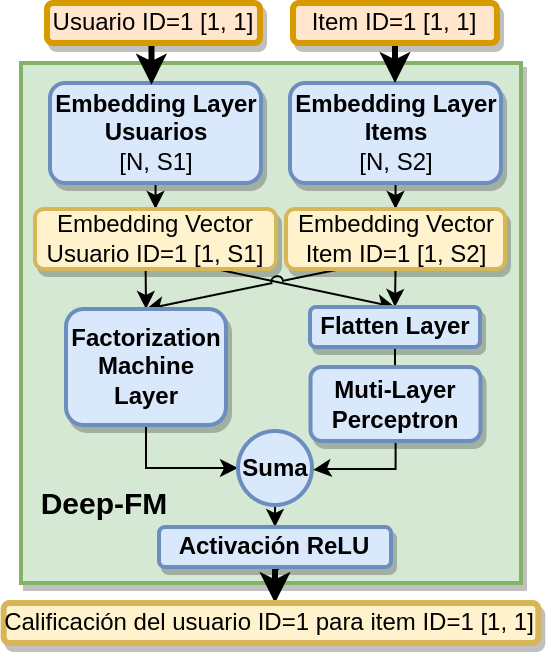
\includegraphics[width=6cm]{./images/Deep-MF.png}
	\caption{
		Esquema de un modelo \textit{Deep Factorization Machine (DeepFM)~\cite{dfmpaper, didldfm}} o maquina
		de factorización basada en \textit{Deep Learning}.
	}
	\label{fig:DeepMFModel}
\end{figure}

Donde se puede apreciar que las entradas del modelo son las variables
categóricas correspondiente a usuarios e ítems, como en los modelos previamente
visto. Dado un identificador de usuario e ítem, se resuelve sus correspondientes
vectores \textit{Embedding}, los cuales se convierten en entradas para los
siguientes dos bloques. Uno de los bloques intermedios, no es mas que una red
neuronal multi capa con capas densas o \textit{fully connected}. Por el otro
lado, ambos vectores se toman como entrada a la máquina de factorización. Las
salidas de ambos bloques intermedios, de valores escalares, se suman y se pasan
por una activación \textit{ReLU}. Para el caso de estudio de este trabajo, las
salidas o calificaciones toman valores mayores a cero, por esta cuestión es mas
adecuado usar una activación \textit{ReLU} frente a una lineal.


\chapter{Pruebas de evaluación}

En este apartado se describirá detalladamente el tipo de pruebas realizadas y cómo se llevaron a cabo. Para la evaluación, se propone un escenario con una instalación real de la \textit{API Rec Chatbot}, la cual ya se explico en detalle en el apartado \ref{sec:arq-general}. De esta forma, contamos con dicha instalación y su respectivo proceso de entrenamiento (\textit{DAG}), el cual se ejecuta cada \textit{5 min} si se encuentran mas de \textit{50} nuevas iteraciones(calificaciones de los usuarios). El objetivo de la prueba es simular un ambiente real de uso de la \textit{API Rec Chatbot} y evaluar la evolución de las recomendaciones para cada usuario de prueba.

\section{Preparación del ambiente de evaluación}

Se dispone de dos conjuntos de datos: uno para entrenamiento y otro para prueba. Tras realizar el flujo de preprocesamiento descrito en la sección \ref{sec:pre-pro}, se excluyen los usuarios que tienen menos de \textit{20} interacciones. Después de este proceso, obtenemos un conjunto de datos con la siguiente distribución de interacciones máximas por usuario (figura \ref{fig:user-interactions}):

\begin{figure}[h!]
	\centering
	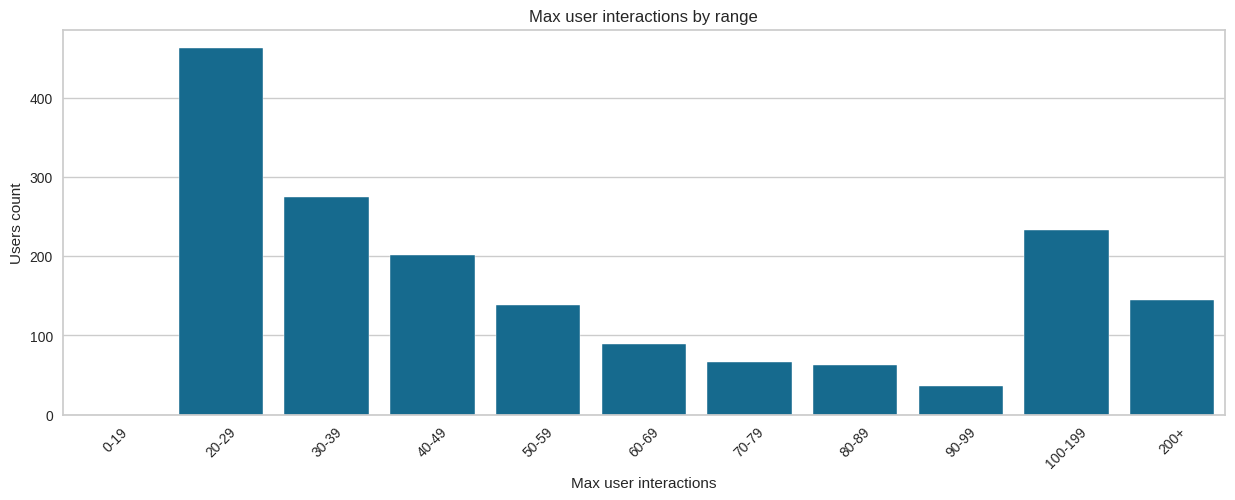
\includegraphics[width=15cm]{./images/user_interactions.png}
	\caption{
		Este gráfico es un histograma que muestra la distribución de interacciones máximas de usuarios. Cada rango representa un rango de interacciones, excluyendo el primer rango de \textit{0} a \textit{19} interacciones. El eje \textit{X} (horizontal) muestra diferentes rangos de interacciones de usuarios, desde \textit{0-19} hasta \textit{200+}. El eje \textit{Y} (vertical) muestra el conteo de usuarios, llegando aproximadamente hasta \textit{450} como máximo por rango.
	}
	\label{fig:user-interactions}
\end{figure}

\textbf{Observaciones}
\begin{itemize}
	\item El pico más alto está en el rango de \textit{20-29} interacciones, con aproximadamente \textit{450} usuarios.
	\item Hay una tendencia general descendente desde ese pico hasta el rango \textit{90-99}.
	\item Existe un segundo pico menor en el rango \textit{100-199}, seguido de una disminución en \textit{200+}.
	\item El rango \textit{0-19} fue filtrado del conjunto de datos, ya que estas interacciones no son buenas para entrenar al modelo.
	\item La mayoría de los usuarios tienen entre \textit{20-29} interacciones.
	\item Es relativamente poco común tener usuarios con más de \textit{100} interacciones.
	\item Hay un grupo interesante de usuarios muy activos en el rango \textit{100-199}.
\end{itemize}

Para construir el conjunto de evaluación se seleccionaron \textit{15} usuarios de cada uno de los siguientes grupos
\textit{20-29}, \textit{30-39}, \textit{40-49}, \textit{50-59}, \textit{60-69}, \textit{70-79}, \textit{80-89}, \textit{90-99} y \textit{100-199}. Excluyendo los grupos \textit{0-19} y \textit{200+} para tratar de representar el comportamiento del usuario promedio, excluyendo comportamientos atípicos o aquellos que no van a permitir realizar una prueba completa del modelo (\textit{0-19}). De esta forma se construye un conjunto de evaluación que represente el comportamiento del usuario promedio, quedando dos conjuntos de entrenamiento y evaluación con la siguiente cantidad de interacciones:

\begin{itemize}
	\item \textbf{Entrenamiento}: \textit{185.096} interacciones (\textit{95\%} el conjunto de datos).
	\item \textbf{Evaluación}: \textit{9.177} (\textit{0.04\%} el conjunto de datos). Este número de interacciones resulta suficiente para realizar la prueba de evaluación y permite utilizar el mayor número posible de interacciones para el entrenamiento del modelo. Ademas debe tenerse en cuenta el tiempo de ejecución de cada inferencia del modelo. Este ronda entre los \textit{8} y \textit{20} segundos. Debido a esto último, tampoco seria posible realizar un particionamiento tradicional \textit{70-30} ya que tendríamos un numero muy grande de interacciones a evaluar.
\end{itemize}

Por otro lado, se agregaron interacciones de usuarios falsos, conocidos como usuarios \textit{fun}. Estos usuarios son entusiastas de ciertos géneros, sagas de películas, etc. Esto usuarios se crean de manera artificial para mejorar las recomendaciones de los modelos de recomendación de filtrado colaborativo, especialmente en casos donde hay grupos de usuarios aislados que no se relacionan entre sí. Para llevar a cabo este proceso, se buscaron ítems a partir de una frase y luego se creo un nuevo usuario al que se asocia una interacción por cada ítem encontrado. A continuación, se muestra el mapeo de frases y la cantidad de ítems obtenidos en cada búsqueda. Cada frase corresponde a un usuario \textit{fun}.

\begin{itemize}
	\item "pixar animated movie for children" (Máximo de 200 items).
	\item "science fiction, action" (Máximo de 100 items).
	\item "war weapons" (Máximo de 70 items).
	\item "iron man, x-men, spider man, bat man, flash, avengers, ant-man, hulk, guardians of the galaxy, marvel, green lantern, superman, watchmen, thor, deadpool, wonder woman, strange, justice League, captain america, logans, kick ass, John Wick" (Máximo de 150 items).
	\item "sci-fi, action, future" (Máximo de 130 items).
	\item "Mission Impossible, spies, bourne identity, 007" (Máximo de 70 items).
	\item "comedy movies" (Máximo de 200 items).
	\item "horror" (Máximo de 100 items).
	\item "thiller, suspense" (Máximo de 150 items).
	\item "love, romance" (Máximo de 150 items).
	\item "time travel" (Máximo de 100 items).
	\item "dead, zombies, post apocalyptic" (Máximo de 100 items).
	\item "software" (Máximo de 100 items).
	\item "hackers" (Máximo de 100 items).
\end{itemize}

De esta forma, se agregan \textit{14} nuevos usuarios artificiales o usuarios \textit{fun}, junto con sus interacciones, al conjunto de datos de entrenamiento.

Para realizar el proceso de evaluación, en primer lugar se deben crear los perfiles de los usuarios encontrados en el conjunto de evaluación. Dado que no se cuenta con información de los mismos. Para realizar esto se generan datos falsos, de forma aleatoria, para el nombre y \textit{email} del usuario. Por otro lado se definen los campos \textit{preferred\_from} y
\textit{genres} que también son parte del perfil de usuario:


\begin{itemize}
	\item \textit{preferred\_from}: Este filtro establece la fecha mínima de lanzamiento de las películas recomendadas. Basándose en las iteraciones de evaluación de cada usuario, se selecciona la fecha de lanzamiento más temprana entre todas las películas que el usuario calificó.
	\item \textit{géneros}: Es una colección de los géneros preferidos por el usuario, al menos inicialmente, similar al campo anterior. Se utiliza un conjunto de todos los géneros.ros de las películas calificadas pro el usuario en el conjunto de evaluación.
\end{itemize}


una vez creados todo los perfiles se dan de alta en \textit{API Rec Chatbot} mediante el \textit{end-point POST /api/v1/profiles}.

Cabe aclarar que estos usuarios no están en el conjunto de entrenamiento; son nuevos para la \textit{API Rec Chatbot}. Además, los usuarios e interacciones presentes en la base de datos de \textit{API Rec Chatbot} pertenecen en su totalidad al conjunto de entrenamiento. A este momento tenemos la base de datos con el conjunto completo de entrenamiento y cargados los perfiles de usuarios del conjunto de evaluación.

\section{Proceso de evaluación}

El proceso de evaluación simula las interacciones de los usuarios con el \textit{API Rec Chatbot}. Se selecciona aleatoriamente y sin reposición cada usuario del conjunto de evaluación, y se itera sobre sus interacciones en orden cronológico, creando consultas a el \textit{API Rec Chatbot} en grupos de \textit{5} interacciones una a la vez. Las consultas o \textit{prompts} tienen el siguiente patrón:

\begin{center}I want to see: title1,..title5\end{center}

Aquí se aprecia que se concatena la cadena de caracteres "I want to see: " con los títulos de las \textit{5} películas correspondientes a las interacciones del usuario a evaluar. Luego, \textit{API Rec Chatbot} buscará y recomendará al menos \textit{5} películas, incluyendo la opción de calificar cada una con una puntuación de \textit{1} a \textit{5}. Las puntuaciones reales del conjunto de evaluación se utilizarán para calificar las recomendaciones. Este proceso se repetirá con las siguientes \textit{5} películas, en el orden cronológico de las interacciones, hasta que se agoten las interacciones del usuario o se alcance un límite de re-intentos en caso de errores con la \textit{API Rec Chatbot}.

Mientras se realiza la prueba de evaluación durante el entrenamiento de la solución, se identifican nuevas interacciones y se decide si es necesario re-entrenar el modelo. El modelo se re-entrena cuando se detectan al menos \textit{25} nuevas interacciones, garantizando así que no haya un desfase significativo. En aplicaciones reales, re-entrenar el modelo cada vez que un usuario califica no es viable debido a los altos requerimientos computacionales, lo que resulta insostenible en términos de \textit{hardware} y costos. Por ello, se opta por un enfoque de entrenamiento en paralelo. El proceso de evaluación continuará hasta alcanzar un mínimo de \textit{50} interacciones por usuario.

El \textit{API Rec Chatbot} consiste en un ensamble de modelos que utiliza modelos de lenguaje para la inferencia. Por ello, se decidió evaluar el sistema dos veces, utilizando dos versiones diferentes del modelo \textit{Llama}: \textit{Llama2} y \textit{Llama3}. Esta selección se realizó tras una prueba temprana donde se compararon distintas implementaciones de modelos de lenguaje, eligiendo estos dos por su consistencia en las respuestas. No todos los modelos de lenguaje ofrecen respuestas consistentes, lo que puede provocar errores en el \textit{parsing} y hacer que el \textit{API Rec Chatbot} no retorne recomendaciones el \textit{100\%} de las veces.


\section{Métricas}

El proceso de evaluación descrito anteriormente registrará los resultados de cada interacción de los usuarios del conjunto de evaluación con  \textit{API Rec Chatbot}, generando un archivo que contendrá los datos necesarios para calcular métricas que permitan evaluar el rendimiento del sistema de recomendación. A continuación se definen todas las métricas utilizadas para facilitar una comprensión inicial. Esto permitirá entender mejor los resultados y las conclusiones de este trabajo de tesis.

\subsection{NDCG (Normalized Discounted Cumulative Gain)}


El \textit{Normalized Discounted Cumulative Gain (NDCG)} es una métrica de evaluación común en el aprendizaje automático, especialmente en tareas de \textit{ranking} o sistemas de recomendación. Esta métrica mide la calidad de una lista ordenada de resultados, teniendo en cuenta no solo si los elementos relevantes están presentes en la lista, sino también su posición. Se basa en dos principios fundamentales:

\begin{itemize}
	\item Los ítems altamente relevantes son más útiles cuando aparecen primeros en la lista de recomendaciones.
	\item Los ítems altamente relevantes son más útiles que los marginal-mente relevantes.
\end{itemize}

\subsubsection{Funcionamiento}

A continuación definimos \textit{NDCG} como:

\begin{equation}
	\begin{split}
		DCG  & = \sum_{i=1}^{n} \frac{rating_i}{\log_2(i + 1)}         \\
		IDCG & = \sum_{i=1}^{n} \frac{rating_i^{ideal}}{\log_2(i + 1)} \\
		NDCG & = \frac{DCG}{IDCG}
	\end{split}
\end{equation}

Donde:
\begin{itemize}
	\item $n$ es la cantidad de ítems en la lista de recomendaciones.
	\item $rating_i$ es la calificación del ítem en la posición $i$ de dicha lista.
	\item $rating_i^{ideal}$ también representa una calificación, pero se basa en una lista ordenada de mayor a menor calificación, lo que significa que el ítem en la posición $i$ podría ser diferente al ítem de la lista original.
\end{itemize}

Primero, se calcula el \textit{DCG (Discounted Cumulative Gain)}:

\begin{itemize}
	\item Para cada ítem \textit{i} de la lista de recomendada, se divide su \textit{rating} o calificación por el logaritmo de su posición en la lista de recomendaciones ($\log_2(i + 1)$). El logaritmo en base \textit{2} de la posición actúa se utiliza como un factor de descuento.
	\item Los ítems en las primeras posiciones de la lista están menos penalizadas por el factor de descuento. Cuanto mayor es el valor de esta división, mas relevante es el ítem para la métrica.
	\item Finalmente se suman todos los valores calculados para cada ítem en la lista, siento este valor final una medida del \textit{Discounted Cumulative Gain}.
\end{itemize}

Luego, es necesario calcular el \textit{IDCG (\textit{Discounted Cumulative Gain} ideal)}:

\begin{itemize}
	\item Se ordenan los ítems de la lista por \textit{rating} o calificación de mayor a menor.
	\item Se calcula el \textit{DCG (Discounted Cumulative Gain)} con este orden ideal.
\end{itemize}

Como paso final, se normaliza el \textit{DCG} dividiendo por el \textit{IDCG}. Esto escala \textit{DCG} a un valor entre \textit{0} y \textit{1}, donde:

\begin{itemize}
	\item \textit{1} indica que la posición de los ítems en la lista(\textit{ranking}) es igual al ideal. Es decir, los ítems están ordenados descendente-mente por la califican que el usuario le a dado.
	\item \textit{0} indica el peor \textit{ranking} posible, es decir seria el orden inverso al \textit{ranking} ideal.
\end{itemize}

\subsubsection{Ejemplo práctico}

Supongamos que contamos con dos sistemas de recomendación de películas, donde ambos miden la relevancia con una puntuación entre \textit{0} a \textit{3} puntos. Luego obtenemos las recomendaciones de ambos sistemas como sigue:

\begin{itemize}
	\item Sistema $A$ recomienda:
	      \begin{itemize}
		      \item Película muy relevante (3 puntos)
		      \item Película poco relevante (1 punto)
		      \item Película relevante (2 puntos)
	      \end{itemize}

	\item Sistema $B$ recomienda:
	      \begin{itemize}
		      \item Película poco relevante (1 punto)
		      \item Película relevante (2 puntos)
		      \item  Película muy relevante (3 puntos)
	      \end{itemize}
\end{itemize}

Aunque ambos sistemas recomiendan las mismas películas, el Sistema $A$ tendrá un \textit{NDCG} mayor, porque ubicó la película más relevante o mayor puntuada al principio. Esto refleja una mejor experiencia de usuario, ya que encontrará contenido más relevante.

\subsection{Exhaustividad \textit{(Recall)}}

Mide la capacidad del sistema para encontrar todos los ítems relevantes para el usuario. Se enfoca en evaluar cuántos de los ítems que realmente le interesan al usuario fueron recomendados. No considera el orden de las recomendaciones ni la precisión con ítems no relevantes.

\subsubsection{Funcionamiento}

A continuación definimos \textit{(Recall)} como:

\begin{equation}
	\text{True Positive} = \text{Ítems Recomendados} \cap \text{Ítems Relevantes}
	\label{eq:tp}
\end{equation}

\begin{equation}
	\text{True Positive} + \text{False Negative} = \text{Ítems Relevantes}
	\label{eq:tp_fn}
\end{equation}

\begin{equation}
	\text{Recall} = \frac{\text{True Positive}}{\text{True Positive} + \text{False Negative}}
	\label{eq:recall}
\end{equation}

Entonces, los pasos para calcular el \textit{(Recall)} son los siguientes:

\begin{itemize}
	\item Se identifica el conjunto de ítems relevantes para el usuario. En el caso de la prueba de evaluación, son todos los ítems utilizados para construir el \textit{prompt} de consulta.
	\item Se cuenta cuántos de estos ítems relevantes aparecen en la lista de ítems recomendados resultado de la consulta \ref{eq:tp}.
	\item Se divide por el número total de ítems relevantes \ref{eq:recall}.
	\item El resultado es un valor entre $0$ y $1$ donde:
	      \begin{itemize}
		      \item El valor $1$ indica que todos los ítems recomendados eran relevantes para el usuario, lo que en la prueba de evaluación significa que todos los ítems coincidían con los utilizados para generar el \textit{prompt} de la consulta.
		      \item El valor $0$ significa que no se recomendó ningún ítem relevante. Lo que significa que ningún de los ítems recomendados se encontraban en el \textit{prompt} de la consulta.
	      \end{itemize}
\end{itemize}

\subsubsection{Ejemplo práctico}
En una aplicación de venta de libros \textit{online}, un usuario está interesado en $5$ libros de ciencia ficción. El sistema le recomienda $5$ libros, de los cuales $3$ son de los que le interesan.

\begin{equation}
	\text{Recall} = \frac{\text{True Positive}}{\text{True Positive} + \text{False Negative}} = \frac{3}{5} = 0.6 = 60\%
\end{equation}

Esto indica que el sistema encontró más de la mitad de los libros que le interesaban al usuario, pero se perdió dos títulos relevantes.

\subsection{Mean Reciprocal Rank (MRR)}

El \textit{MRR} se usa para evaluar la eficacia de un sistema de recomendación o motor de búsqueda en términos de cuán cerca del inicio en los resultados se encuentran los ítems relevantes para los usuarios. Un \textit{MRR} alto sugiere que el sistema está bien optimizado para mostrar los resultados más relevantes en las primeras posiciones, mientras que un valor más bajo indica que los usuarios deben revisar más resultados para encontrar lo que buscan.

\subsubsection{Funcionamiento}

La métrica se define como sigue:

\begin{equation}
	MRR= \frac{1}{|U|} \sum_{u=1}^{|U|} \frac{1}{rank_u}
\end{equation}

Donde:

\begin{itemize}
	\item $|U|$ es el número total de usuarios registrados en el sistema de recomendación.
	\item $rank_u$ es la posición del primer ítem relevante para el usuario $u$ dentro de una lista de ítems recomendada por el sistema de recomendación.
\end{itemize}

Entonces, para cada usuario:

\begin{itemize}
	\item Se encuentra la posición del primer ítem relevante ($rank_u$) en la lista recomendada.
	\item Se calcula el recíproco de esta posición ($1/rank_u$).
\end{itemize}

Luego, se promedian todos los valores calculados para cada usuario de la siguiente manera:
\begin{itemize}
	\item Se suman todos los recíprocos.
	\item Se divide el total por el número de usuarios ($|U|$).
\end{itemize}

El resultado será un valor entre $0$ y $1$, donde:
\begin{itemize}
	\item $1$ significa que el primer ítem fue relevante para todos los usuarios.
	\item Valores cercanos a $0$ indican que los ítems relevantes aparecen en las ultima posiciones en la lista de ítems recomendados a cada usuario.
\end{itemize}


\subsubsection{Ejemplo práctico}

En un buscador de restaurantes:
\begin{itemize}
	\item El usuario 1 encuentra el primer restaurante relevante en la $2da$ posición ($1/2$).
	\item El usuario 2 encuentra el primer restaurante relevante en la $1ra$ posición ($1/1$).
	\item El usuario 3 encuentra el primer restaurante relevante en la $4ta$ posición ($1/4$)
\end{itemize}

\begin{equation}
	MRR = \frac{1/2 + 1/1 + 1/4}{3} = 0.58
\end{equation}

Esto indica que, en promedio, los usuarios encuentran un restaurante relevante en la segunda posición, ya que $0.58 \approx 1/2$, donde 2 es la posición.


\subsection{Mean Average Precision (MAP)}

Es una métrica comúnmente utilizada para evaluar la precisión de un sistema de recomendación, un motor de búsqueda, o un modelo de clasificación. En términos simples, \textit{MAP} mide la precisión de un modelo al identificar elementos relevantes entre los resultados y lo hace promediando la precisión en diferentes niveles de relevancia a lo largo de las búsquedas de múltiples usuarios o consultas. Es más rigurosa que el \textit{Recall} ya que considera la posición en que aparecen los ítems relevantes.

\subsubsection{Cálculo del \textit{MAP}}

\begin{enumerate}
	\item \textit{Average Precision (AP)} para una consulta individual: Para cada consulta o búsqueda, se calcula el \textit{Average Precision (AP)}, que es el promedio de la precisión en cada posición donde aparece un ítem relevante. La precisión en una posición \( k \) es la fracción de ítems relevantes entre los primeros \( k \) resultados.

	      La fórmula para el \textit{AP} de una consulta es la siguiente:

	      \[
		      \text{Precisión@k} = \frac{\text{Cantidad de ítem relevantes encontrados hasta k}}{k}
	      \]
	      \[
		      AP = \frac{1}{\text{Cantidad total de ítems relevantes}} \sum_{k=1}^{n} \text{Precisión@k} \times \text{Relevancia de ítem k}
	      \]
	      Donde:
	      \begin{itemize}
		      \item $n$: Es el número total de ítems en la lista recomendada al usuario.
		      \item \text{Precisión@k}: Se define como el número de ítems relevantes encontrados en los primeros \( k \) ítems, dividido por el total de ítems analizados hasta el momento ($k$). Por ejemplo, si se analizan los primeros \( k=3 \) ítems y se encuentra un ítem relevante entre estos, la \text{precisión@k} es igual a \( 1/3 \).
		      \item \text{Relevancia en} k: Toma el valor 1 si el ítem en la posición \( k \) es relevante y $0$ si no lo es. Esto permite filtrar los ítems irrelevantes, enfocándonos únicamente en las precisiones de los ítems relevantes.
		      \item Finalmente, se suman las precisiones en las posiciones donde el ítem es relevante, y luego se divide por el número total de ítems relevantes para esa lista recomendada.
	      \end{itemize}

	\item \textit{MAP} es el promedio de los \textit{AP's}: Tras calcular el \textit{AP} de cada lista recomendada, se promedian estos valores para obtener el \textit{MAP}. Esto refleja el promedio de los \textit{AP's} para todos los usuarios del sistema de recomendación, donde se consulta una recomendación para cada uno de ellos.

	      La fórmula es la siguiente:
	      \[
		      MAP = \frac{1}{Q} \sum_{q=1}^{Q} AP_q
	      \]
	      Donde:
	      \begin{itemize}
		      \item \( Q \) es el número total de consultas de recomendaciones o usuarios. Si tenemos $n$ usuarios se debe consultar una recomendación de ítems por cada uno.
		      \item \( AP_q \) es el \textit{Average Precision} de la consulta \( q \).
	      \end{itemize}
\end{enumerate}

\subsubsection{Ejemplo de Cálculo de \textit{MAP}}

Imaginemos que tenemos 3 usuarios que buscan restaurantes, y los resultados relevantes aparecen en las siguientes posiciones:

\begin{itemize}
	\item El usuario 1 encuentra ítems relevantes en las posiciones $1$ y $3$.
	\item El usuario 2 encuentra ítems relevantes en las posiciones $2$ y $4$.
	\item El usuario 3 encuentra un ítem relevante en la posición $1$.
\end{itemize}

Cálculo de \textit{AP} para cada usuario:

\begin{itemize}
	\item Usuario 1:
	      \begin{align*}
		      \text{Precisión en posición 1} & = \frac{1}{1} = 1            \\
		      \text{Precisión en posición 3} & = \frac{2}{3} \approx 0.67   \\
		      AP_1                           & = \frac{1 + 0.67}{2} = 0.835
	      \end{align*}

	\item Usuario 2:
	      \begin{align*}
		      \text{Precisión en posición 2} & = \frac{1}{2} = 0.5         \\
		      \text{Precisión en posición 4} & = \frac{2}{4} = 0.5         \\
		      AP_2                           & = \frac{0.5 + 0.5}{2} = 0.5
	      \end{align*}

	\item Usuario 3:
	      \begin{align*}
		      \text{Precisión en posición 1} & = \frac{1}{1} = 1 \\
		      AP_3                           & = 1
	      \end{align*}
\end{itemize}

Cálculo del \textit{MAP}:

\[
	MAP = \frac{AP_1 + AP_2 + AP_3}{3} = \frac{0.835 + 0.5 + 1}{3} \approx 0.778
\]

Interpretación del \textit{MAP}:

\begin{itemize}
	\item Un \textit{MAP} cercano a 1 significa que los ítems relevantes suelen aparecer en las primeras posiciones para todos los usuarios, indicando alta precisión del sistema.
	\item Un \textit{MAP} cercano a 0 sugiere que los ítems relevantes están, en promedio, en posiciones bajas, indicando que el sistema podría mejorar en términos de precisión y relevancia en los primeros resultados.
\end{itemize}


\subsection{Catalog Coverage}

La métrica \textit{Catalog Coverage} (Cobertura del Catálogo) mide qué tan amplio es el rango de ítems o productos que un sistema de recomendación muestra a los usuarios. En pocas palabras, representa la diversidad del catálogo que es recomendado a través de todas las interacciones con los usuarios. Esta métrica es importante para asegurar que el sistema no se enfoque únicamente en un conjunto pequeño de productos populares, sino que exponga a los usuarios a una gama más amplia de opciones disponibles en el catálogo.

\subsubsection{¿Por qué es importante Catalog Coverage?}
\begin{itemize}
	\item Diversidad: Un alto \textit{Catalog Coverage} asegura que el sistema de recomendación promueva ítems diversos, en lugar de solo aquellos que ya son populares.
	\item Satisfacción del usuario: Al ofrecer una variedad más amplia de ítems, es más probable que los usuarios encuentren productos específicos que se ajusten a sus intereses únicos.
	\item Valor de negocio: Promover más ítems del catálogo puede llevar a aumentar las ventas de productos menos conocidos o de "larga cola", maximizando el uso de todo el inventario.
\end{itemize}



\subsubsection{Cálculo de \textit{Catalog Coverage}}

\textit{Catalog Coverage} se expresa como el porcentaje de ítems únicos que se recomiendan al menos una vez en relación con el total de ítems disponibles en el catálogo. Su fórmula es la siguiente:

\[
	\text{Catalog Coverage} = \frac{\text{Número de ítems únicos recomendados}}{\text{Número total de ítems en el catálogo}}
\]

Donde:
\begin{itemize}
	\item \textit{Número de ítems únicos recomendados} es el conteo de los ítems que fueron recomendados al menos una vez en todas las interacciones con los usuarios.
	\item \textit{Número total de ítems en el catálogo} es el total de ítems que el sistema podría recomendar.
\end{itemize}

\subsubsection{Ejemplo de Cálculo}

Imaginemos que tenemos un catálogo de 1000 ítems (productos, películas, etc.), y un sistema de recomendación que ha recomendado 200 de estos ítems en total a los usuarios.

\[
	\text{Catalog Coverage} = \frac{200}{1000} = 0.2 \quad \text{o bien, } 20\%
\]

Esto indica que el sistema de recomendación utiliza solo el 20\% del catálogo en sus recomendaciones. Un Catalog Coverage más alto (por ejemplo, 80\%) reflejaría que el sistema está recomendando una mayor variedad de ítems, mientras que un valor bajo puede indicar que el sistema se enfoca en un subconjunto limitado.

\subsubsection{Interpretación de Catalog Coverage}

\begin{itemize}
	\item Un alto \textit{Catalog Coverage} (por ejemplo, 70\%-100\%): El sistema cubre una amplia gama del catálogo, lo cual puede ser positivo en términos de diversidad y satisfacción del usuario.
	\item Un bajo \textbf{Catalog Coverage} (por ejemplo, 0\%-30\%): El sistema utiliza solo una pequeña parte del catálogo, lo que puede llevar a una experiencia limitada y potencialmente menos interesante para los usuarios.
\end{itemize}

\subsubsection{Limitaciones}

Aunque un alto \textit{Catalog Coverage} puede mejorar la experiencia del usuario, no siempre es ideal si esto implica recomendar productos menos relevantes. Es necesario un balance para mantener tanto la diversidad como la relevancia en las recomendaciones.


\subsection{Serendipity}

La \textit{Serendipity} o serendipia en sistemas de recomendación se refiere a la capacidad de un sistema para proporcionar a los usuarios recomendaciones inesperadas pero valiosas que no buscaban inicialmente. Este concepto está relacionado con la sorpresa positiva y la satisfacción que puede generar el descubrimiento de ítems o productos que son relevantes para el usuario, aunque no fueran explícitamente solicitados.

\subsubsection*{Importancia de la \textit{Serendipity}}

\begin{itemize}
	\item Experiencia del usuario: Las recomendaciones serendipitosas pueden enriquecer la experiencia del usuario al exponerlo a opciones que no había considerado, aumentando su satisfacción y \textit{engagement} con el sistema.
	\item Fidelización: Al sorprender a los usuarios con recomendaciones relevantes, se incrementa la probabilidad de que regresen al sistema, mejorando la lealtad del cliente.
	\item Diversidad: Promover la serendipia ayuda a diversificar las opciones que se muestran, evitando que el sistema se centre únicamente en ítems populares o en las preferencias ya conocidas del usuario.
\end{itemize}

\subsubsection*{Cálculo y Medición de \textit{Serendipity}}

\begin{equation}
	Serendipity = \frac{1}{|U|} \sum_{u=1}^{|U|} \frac{|UNEXP_u \cap REL_u \cap REC_u|}{k}
\end{equation}

Donde:
\begin{itemize}
	\item $|U|$ es el número de usuarios.
	\item $UNEXP_u$ es el conjunto de ítems inesperados para el usuario $u$.
	\item $REL_u$ es el conjunto de ítems relevantes para el usuario $u$.
	\item $REC_u$ es el conjunto de ítems recomendados al usuario $u$.
	\item $k$ es el número de recomendaciones consideradas.
\end{itemize}


Entonces, para cada usuario:

\begin{itemize}
	\item Se identifican los ítems recomendados($REC_u$) en el top-k.
	\item Se identifican los ítems relevantes($REL_u$).
	\item Se identifican los ítems inesperados($UNEXP_u$), el complemento de los dos primeros.
	\item Se cuenta cuántos ítems cumplen las tres condiciones.
	\item Se divide por $k$.
	\item Se promedian los valores de todos los usuarios ($|U|$).
\end{itemize}

El resultado es un valor entre $0$ y $1$ donde:
\begin{itemize}
	\item $1$ indica que todas las recomendaciones son relevantes e inesperadas.
	\item $0$ indica que no hay recomendaciones serendípicas.
\end{itemize}



\subsubsection*{Limitaciones}

A pesar de los beneficios, la serendipia debe equilibrarse con la relevancia. Si un sistema ofrece demasiadas recomendaciones inesperadas que no son relevantes, puede frustrar a los usuarios en lugar de sorprenderlos positivamente.


\subsubsection*{Ejemplo de Cálculo}

Supongamos que tenemos un sistema de recomendación con tres usuarios (\( |U| = 3 \)), y cada usuario tiene un conjunto de ítems recomendados, relevantes, e inesperados. Queremos calcular la serendipia promedio de las recomendaciones para estos usuarios considerando \( k = 5 \) recomendaciones.

Luego para cada usuario tenemos los siguientes ítems:
\begin{itemize}
	\item Usuario 1:
	      \begin{itemize}
		      \item $REC_1 = \{A, B, C, D, E\}$
		      \item $REL_1 = \{A, C, F\}$
		      \item $UNEXP_1 = \{A, C\}$
	      \end{itemize}
	\item Usuario 2:
	      \begin{itemize}
		      \item $REC_2 = \{G, H, I, J, K\}$
		      \item $REL_2 = \{G, H, M\}$
		      \item $UNEXP_2 = \{I, K\}$
	      \end{itemize}
	\item Usuario 3:
	      \begin{itemize}
		      \item $REC_3 = \{N, O, P, Q, R\}$
		      \item $REL_3 = \{N, Q, T\}$
		      \item $UNEXP_3 = \{N, P\}$
	      \end{itemize}
\end{itemize}

Usamos la fórmula de serendipia para cada usuario:
\[
	Serendipity = \frac{1}{|U|} \sum_{u=1}^{|U|} \frac{|UNEXP_u \cap REL_u \cap REC_u|}{k}
\]

Calculamos para cada usuario:
\begin{itemize}
	\item Para el usuario 1: \( UNEXP_1 \cap REL_1 \cap REC_1 = \{C\} \), entonces:
	      \[
		      \frac{|UNEXP_1 \cap REL_1 \cap REC_1|}{k} = \frac{2}{5} = 0.4
	      \]
	\item Para el usuario 2: \( UNEXP_2 \cap REL_2 \cap REC_2 = \{H\} \), entonces:
	      \[
		      \frac{|UNEXP_2 \cap REL_2 \cap REC_2|}{k} = \frac{0}{5} = 0
	      \]
	\item Para el usuario 3: \( UNEXP_3 \cap REL_3 \cap REC_3 = \{Q\} \), entonces:
	      \[
		      \frac{|UNEXP_3 \cap REL_3 \cap REC_3|}{k} = \frac{1}{5} = 0.2
	      \]
\end{itemize}

Finalmente, el valor promedio de serendipia para los tres usuarios es:
\[
	Serendipity = \frac{1}{3} (0.4 + 0 + 0.2) = 0.2
\]


\chapter{Resultados}

En los siguientes capítulos se presentaran los resultados de las pruebas de evaluación para dos configuraciones distintas del sistema de recomendación. Para esto se reemplaza un componente del sistema de recomendación, encargado de aplicar el \textit{ranking} a los ítems que forman parte del resultado de una consulta. Éste componente es un modelo de lenguaje grande  encargado de refinar el ordenamiento de los resultados, el cual se utiliza a lo largo del ciclo de vida del usuario.

Para el sistema de recomendación, el usuario puede tomar dos estados posibles, e ir cambiando entre los mismos dentro de su ciclo de vida. Estos estados definen dos estrategias distintas de recomendación de contenido:

\begin{itemize}
	\item Estado frio (\textit{Cold}): Para los usuarios en este estado, el sistema de recomendación carece de información sobre su comportamiento, ya que este no ha calificado ningún contenido en el ultimo tiempo. En este estado, solo se dispone de información general del perfil del usuario, limitándose a realizar
	      recomendaciones basadas en su perfil y contenido similar a su consulta (estrategia de basada en contenido). En este estado el modelo utiliza un técnica \textit{RAG}(\textit{Retrieval Augmented Generation} o Generación Aumentada por Recuperación) ~\cite{rag} para buscar contenido similar a la consulta del usuario, utilizando la distancia Coseno como primer método de \textit{ranking}. Luego se utiliza un modelo de lenguaje grande para refinar el ordenamiento basándose en los resultado de la técnica \textit{RAG}(\textit{Retrieval Augmented Generation} o Generación Aumentada por Recuperación) ~\cite{rag} e información del perfil del usuario.
	\item Estado caliente (\textit{Warn}): Para los usuarios en este estado, el sistema de recomendación cuenta con un número mínimo de interacciones, utilizadas para realizar recomendaciones basadas en su comportamiento. Se utiliza un modelo de recomendación basado en filtros colaborativos como primer método de búsqueda y ordenamiento(\textit{ranking}) de ítems, seguido por un modelo de lenguaje grande, que refina este ordenamiento en función de las interacciones(calificaciones) del usuario y el perfil del usuario (similar a la estrategia anterior).
\end{itemize}

Es importante mencionar que las interacciones del usuario (calificaciones de ítems) tienen una fecha de expiración, lo que implica una ventana de tiempo hacia atrás desde la fecha actual para considerar su comportamiento. Esto garantiza que el sistema de recomendación refleje las preferencias más recientes del usuario. Además, el sistema alternará entre diferentes estrategias de recomendación según la frecuencia de interacciones. Aunque la evaluación del modelo no tiene en cuenta esta ventana temporal, ya que las interacciones ocurren dentro del período de ejecución de la prueba(del orden de días), es importante señalar que el sistema cuenta con esta capacidad.

\chapter{Resultados utilizando el componente \textit{LLM} \textit{Llama2}}

En esta sección se presentan los resultados de la evaluación del sistema de recomendación, donde se utilizó el componente \textit{Llama2} para refinar el \textit{ranking} de los ítems recomendados a partir de una consulta realizada por un usuario perteneciente al conjunto de evaluación.

Para comenzar, en la figura \ref{fig:llama2-steps_count_by_session_distribution} se muestra la distribución de la cantidad de pasos por sesión de usuario. Un paso representa una recomendación solicitada por un usuario dentro de su sesión y una sesión puede tener $n$ pasos. Se puede apreciar que la mayoría de los usuarios realizan entre $6$ y $13$ consultas por sesión (rango inter-cuartíl), siendo $6$ consultas el valor más común (moda).
Algunos usuarios realizan pocas consultas ($<6$), mientras que un pequeño grupo llega a realizar muchas ($>22$), considerados \textit{outliers} ($4.48\%$ del total). La asimetría positiva indica que la mayoría de los usuarios tienen un comportamiento entre el promedio y la moda, pero existen algunos usuarios con gran cantidad de interacciones (sesiones largas con muchas consultas). La media ($10.59$), mayor que la mediana ($9$), indicando que la distribución esta sesgada hacia la derecha, sugiere que estos usuarios extremos están influyendo en el valor del promedio. Las sesiones con más de $22$ consultas podrían indicar: Usuarios avanzados/expertos que exploran profundamente el sistema.

\begin{figure}[H]
	\centering
	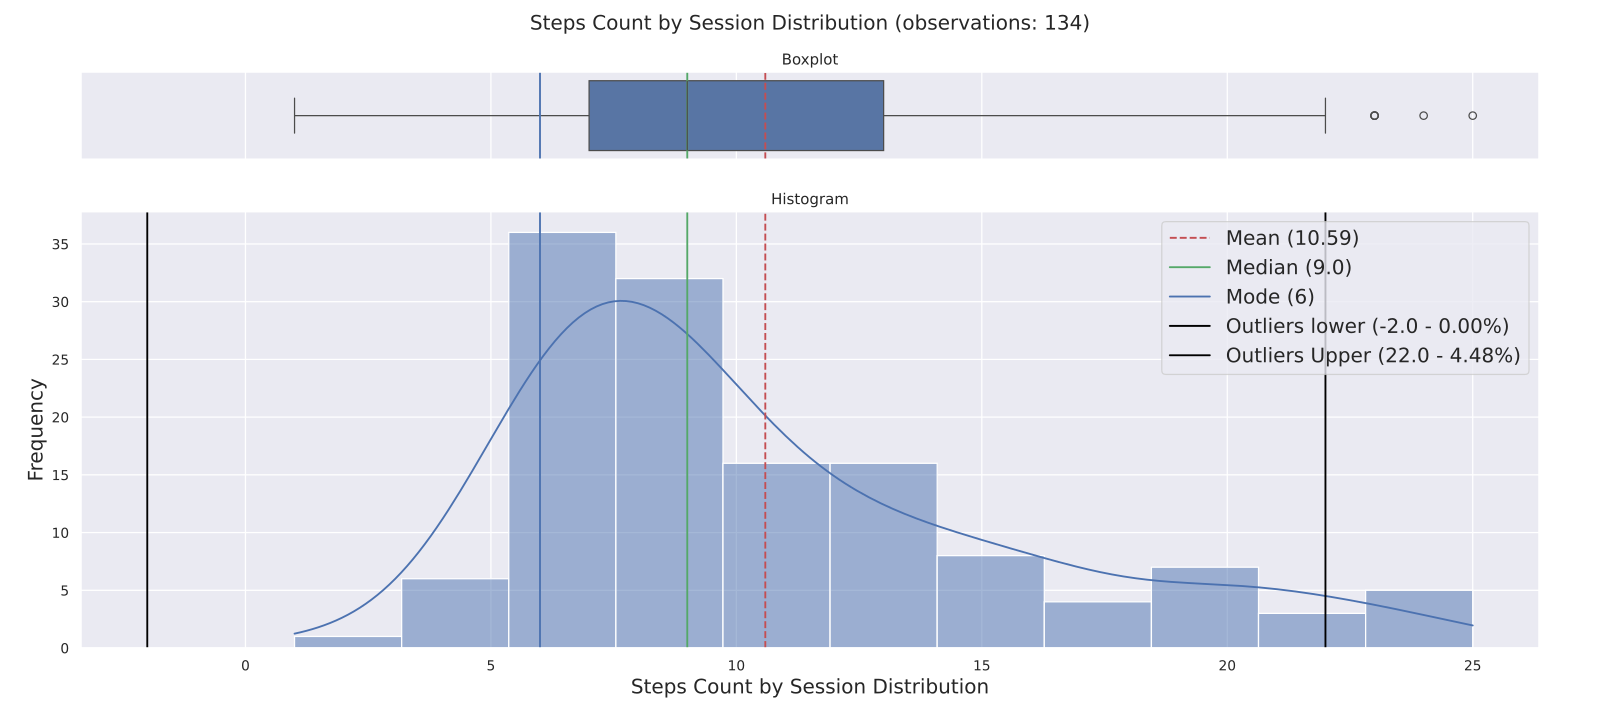
\includegraphics[width=15cm]{./images/llama2/steps_count_by_session_distribution.png}
	\caption{Este gráfico representa la cantidad de pasos por sesión de usuario. Un paso representa una consulta de recomendación realizada por un usuario.}
	\label{fig:llama2-steps_count_by_session_distribution}
\end{figure}

En la figura \ref{fig:llama2-sessions_count_by_session_step} se muestra la cantidad de usuarios(o sesiones activas) por paso. Cada paso es una consulta al sistema de recomendación, indicando una secuencia ordinal de consultas. Es decir, en el paso $1$, se registran $134$ usuarios que realizaron la primera consulta, en el paso $2$, $133$ usuarios y así hasta llegar al ultimo paso ($25$), al cual solo llego un único usuario. Cabe aclarar que la sesión que realiza el paso $25$, también realizo todo los pasos anteriores. Se puede apreciar que se mantiene un nivel muy alto de retención hasta el sexto paso, con solo pequeñas disminuciones.
Se aprecia una caída progresiva después del paso $6$. A partir del séptimo paso, el número de sesiones disminuye de manera constante. En el paso $10$, el número de sesiones ya ha disminuido casi a la mitad ($59$ sesiones). La reducción es más drástica a medida que se avanza, hasta que solo unas pocas sesiones alcanzan o superan los $20$ pasos.
Pocos usuarios llegan a pasos muy altos: A partir del paso $21$, el número de sesiones activas es muy bajo, con menos de $10$ sesiones. Solo una sesión llega al paso $25$.

\begin{figure}[H]
	\centering
	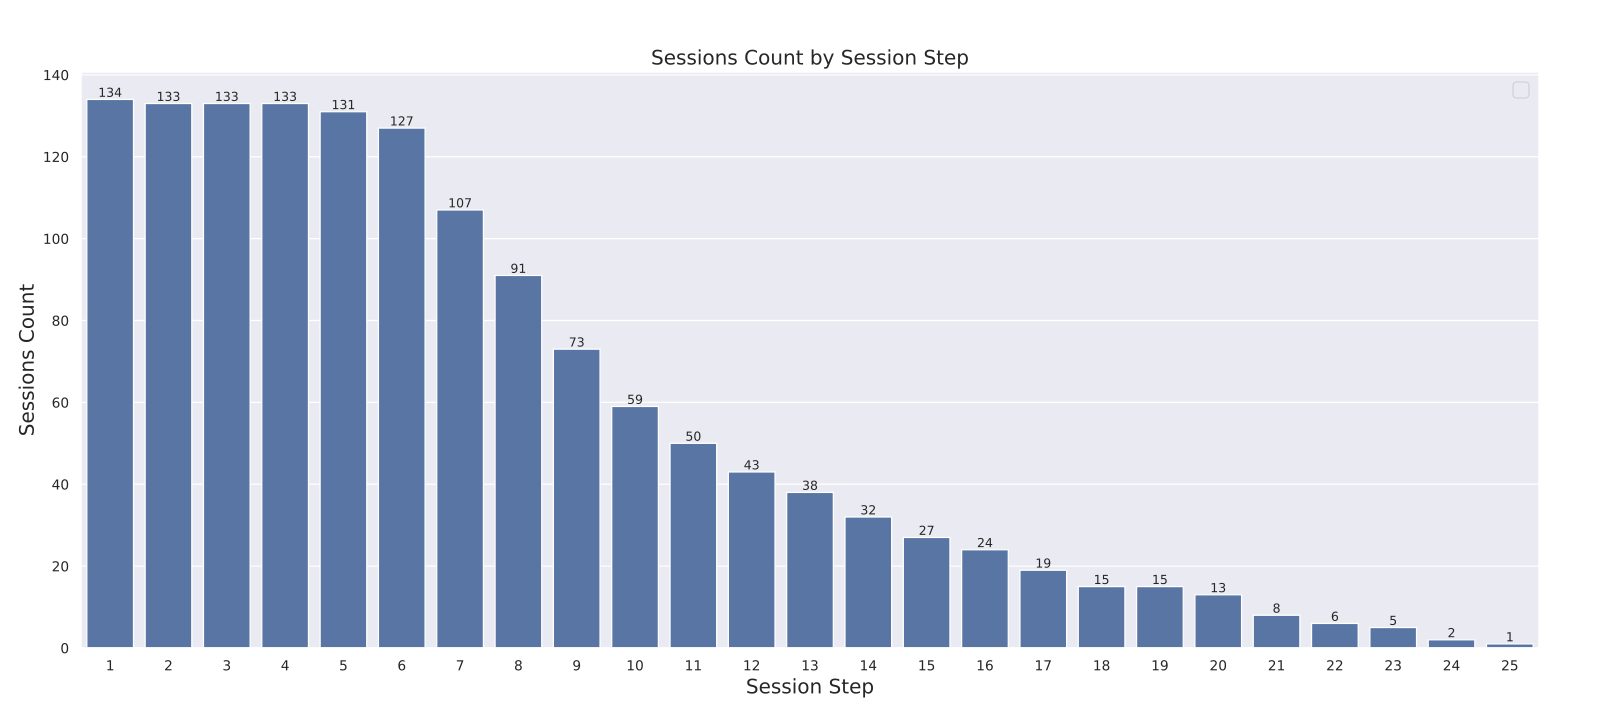
\includegraphics[width=15cm]{./images/llama2/sessions_count_by_session_step.png}
	\caption{Este gráfico muestra el número de sesiones de usuarios por  cada paso de sesión, donde cada paso corresponde a una consulta al sistema de recomendación. Se observa que un usuario llego a realizar $25$ consultas y $134$ usuarios completaron el primer paso.}
	\label{fig:llama2-sessions_count_by_session_step}
\end{figure}

La figura \ref{fig:llama2-found_items_count_by_session_step_distribution} muestra la cantidad de ítems relevantes encontrados en los resultados a consultas de usuario. Los ítems relevantes son aquellos cuya interacción es conocida, mientras que los no relevantes son ítems que el usuario no buscó, pero que aparecen en la lista de recomendaciones, ya sea por su similitud a la consulta o por el grado de preferencia que el sistema de recomendación infiere del usuario.  Cada consulta devuelve un máximo de $5$ ítems relevantes. Los usuarios, por lo general, encuentran entre $2$ y $3$ ítems por paso, lo que indica que el sistema no siempre localiza todos los ítems solicitados. Esto sugiere que se podría mejorar la búsqueda por similitud (\textit{embeddings}). Una opción sería utilizar \textit{embeddings} generados por \textit{gpt-40} de \textit{OpenAI}. Sin embargo, esto no es un indicador definitivo del rendimiento del sistema, ya que puede que no retorne películas por su nombre exacto (como se realiza en esta prueba de evaluación), pero aun así recomendar opciones relevantes y tener buen desempeño en métricas como \textit{MAP@K} u otras especializadas para evaluar el sistema de recomendación.


\begin{figure}[H]
	\centering
	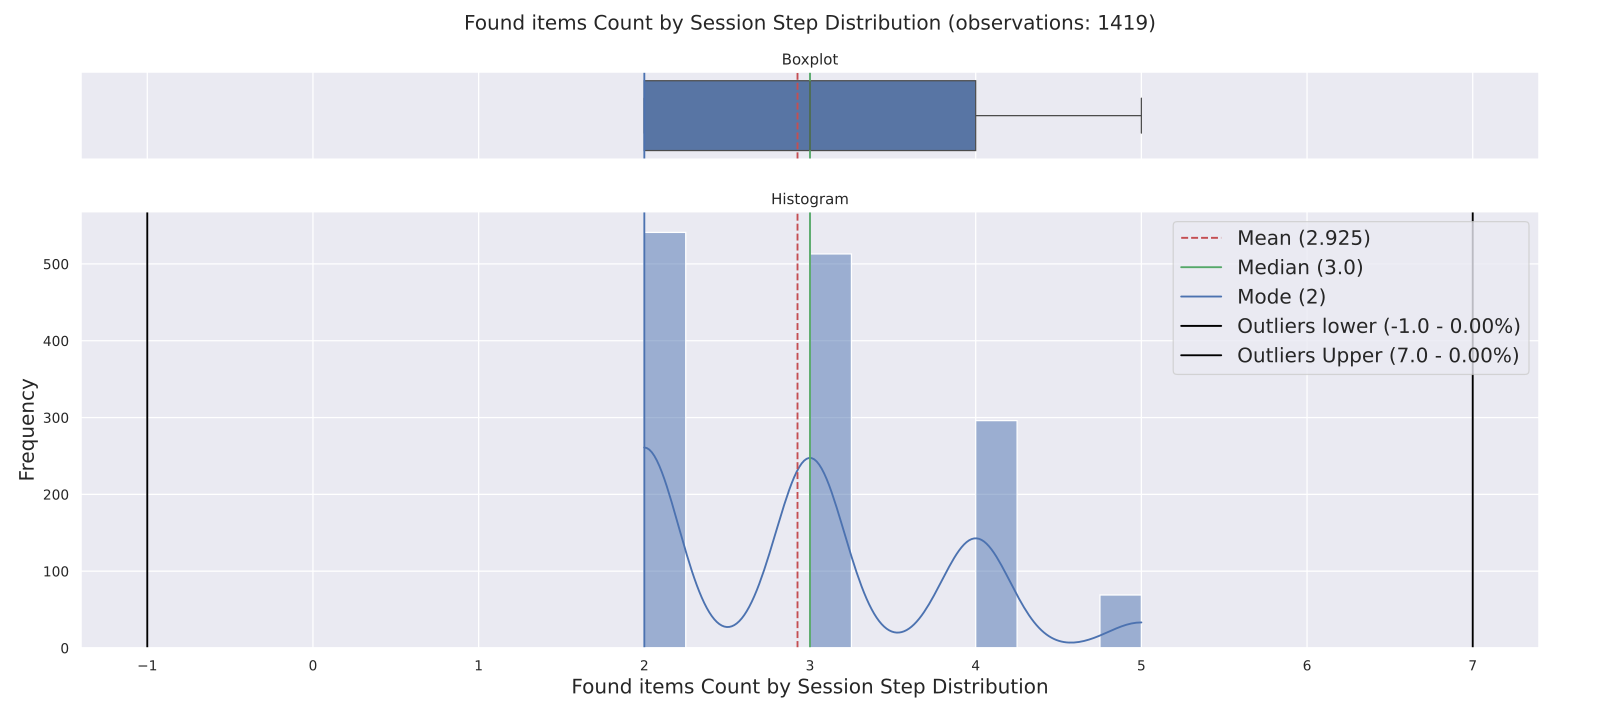
\includegraphics[width=15cm]{./images/llama2/found_items_count_by_session_step_distribution.png}
	\caption{En este gráfico se aprecia la cantidad de ítems relevantes encontrado en cada respuesta del sistema de recomendación. Donde la mayoría de las consultas (Moda) contienen $2$ ítems relevantes con una media de $3$.}
	\label{fig:llama2-found_items_count_by_session_step_distribution}
\end{figure}


En la figura \ref{fig:llama2-mean_average_precision_by_session_distribution} se muestra la distribución de la métrica \textit{Mean Average Precision}(\textit{MAP}) por sesión de usuario. La distribución muestra que la mayoría de los valores de \textit{MAP} se concentran entre $0.45$ y $0.65$, con algunos \textit{outliers} en valores mas altos. Se aprecian valores clave como la media ($0.548$), la mediana ($0.545$) y la moda ($0.58$). La curva de densidad sobre el histograma indica una ligera asimetría positiva (cola hacia la derecha), lo que sugiere que existen sesiones con \textit{MAP} relativamente alto. No hay \textit{outliers} inferiores, pero los valores superiores (por encima de $0.765$) se destacan. Estos puntos podrían indicar sesiones inusuales, tal vez relacionadas con usuarios específicos o películas más populares.

\begin{figure}[H]
	\centering
	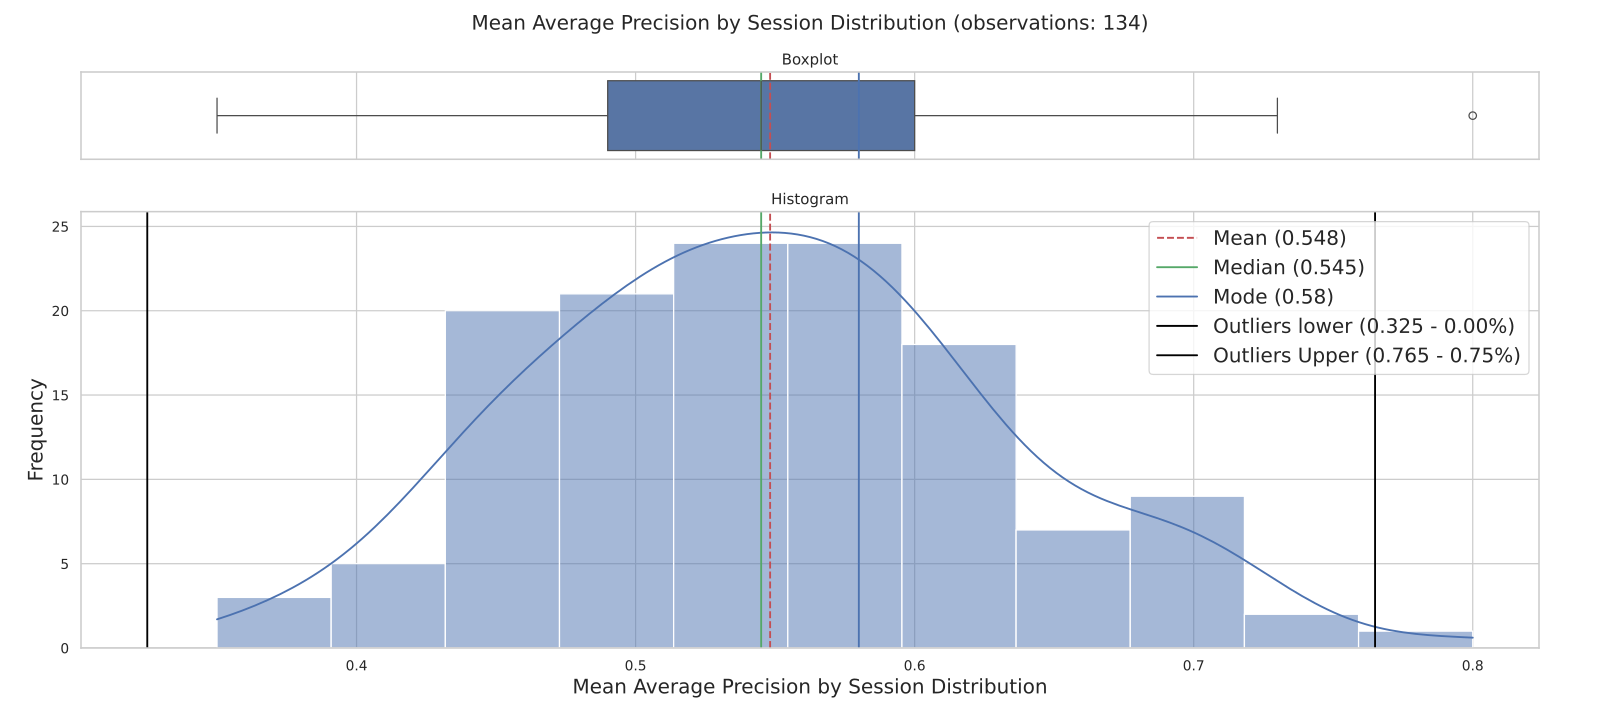
\includegraphics[width=15cm]{./images/llama2/mean_average_precision_by_session_distribution.png}
	\caption{En este gráfico se aprecia la distribución de la métrica \textit{Mean Average Precision}(\textit{MAP}) por sesión de usuario.}
	\label{fig:llama2-mean_average_precision_by_session_distribution}
\end{figure}

\clearpage

En la figura \ref{fig:llama2-mean_average_precision_by_session_step_series} se muestra una serie que describe la evolución  del \textit{Mean Average Precision}(\textit{MAP}) promedio por paso.

\begin{figure}[H]
	\centering
	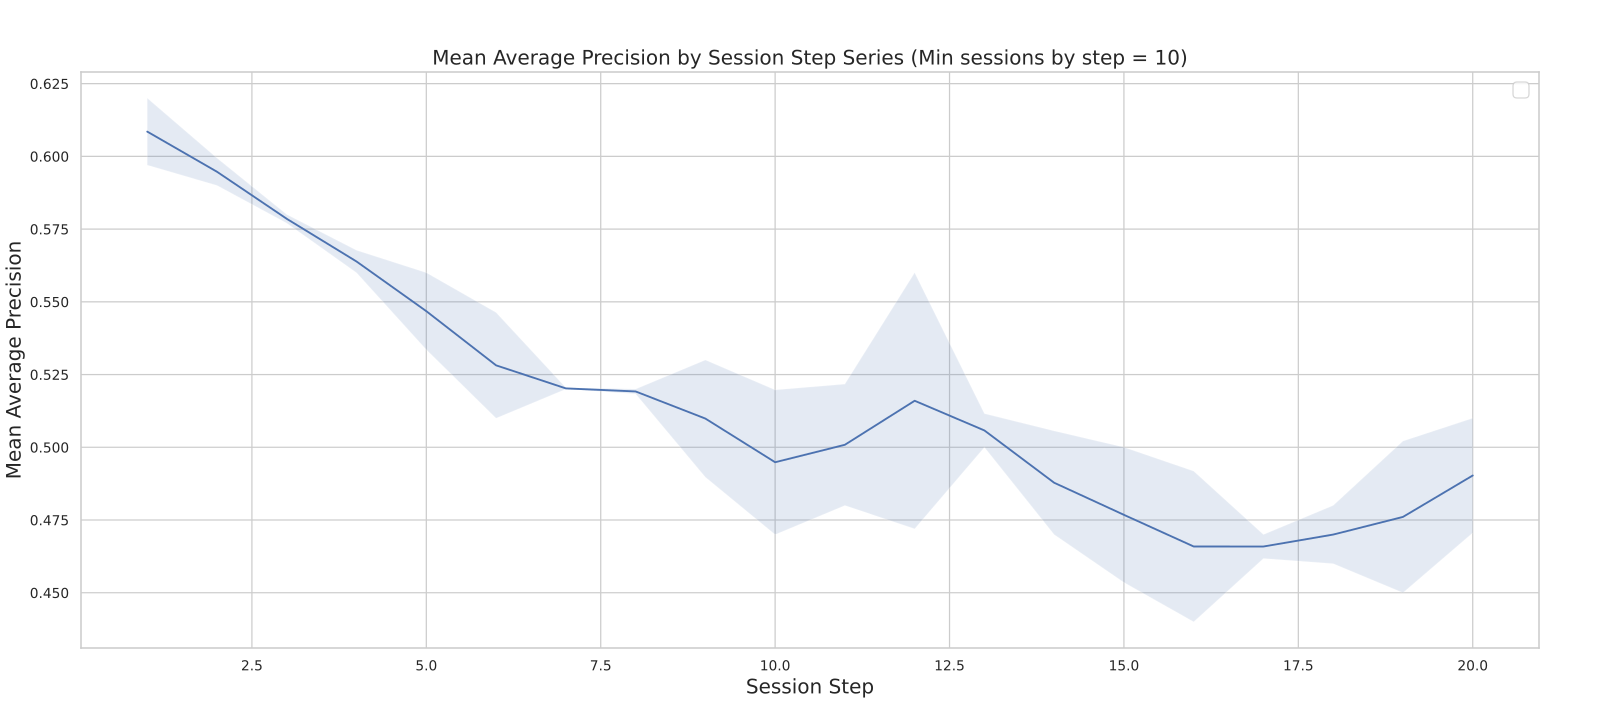
\includegraphics[width=15cm]{./images/llama2/mean_average_precision_by_session_step_series.png}
	\caption{
		En este gráfico se aprecia una serie que muestra la evolución del de \textit{Mean Average Precision}(\textit{MAP}) promedio por paso. Es decir se realiza la media de \textit{Mean Average Precision}(\textit{MAP}) de cada sesión de usuario en cada paso(\textit{Session Step}).}
	\label{fig:llama2-mean_average_precision_by_session_step_series}
\end{figure}

Es decir, se realiza el \textit{Mean Average Precision}(\textit{MAP}) promedio de cada sesión de usuario en cada paso. La línea azul representa el \textit{Mean Average Precision}(\textit{MAP}) promedio por paso de sesión, mientras que el área sombreada muestra la intervalo de confianza o la variabilidad de la métrica. Se observa una tendencia decreciente del \textit{Mean Average Precision}(\textit{MAP}) conforme avanzan los pasos de la sesión (\textit{Session Step}). Esto sugiere que el sistema tiene mayor precisión en las recomendaciones iniciales, pero su desempeño disminuye progresivamente. A partir del paso $10$, la tendencia se estabiliza y muestra ligeros altibajos.
Esto podría implicar que el sistema llega a un límite en la calidad de las recomendaciones después de varios pasos, posiblemente debido a la menor relevancia o diversidad de los ítems sugeridos. Curiosamente, entre los pasos $17$ y $20$, el \textit{Mean Average Precision}(\textit{MAP}) parece mostrar un aumento leve. Esto podría deberse a la disminución de sesiones en estos pasos. Menos sesiones implica mas \textit{leverage} o palanca de valores atípicos altos. El área sombreada es más amplia en los rangos intermedios ($8-12$ y $12-15$), lo que sugiere una mayor dispersión en los valores de \textit{Mean Average Precision}(\textit{MAP}). Esta área corresponde a los pasos donde los usuarios cambian de estado, pasando del estado frio al estado caliente. Este cambio de estrategia utilizada de forma diferenciada por cada usuario puedo estar generando distintos valores de la métrica, produciendo la dispersión observada. Por otro lado, el hecho de que el usuario consulte siempre cinco ítems por su nombre indica que el sistema enfrenta dificultades para realizar esta búsqueda por término.

\clearpage

En la figura \ref{fig:llama2-mean_ndcg_by_session_step_distribution} se muestra la media de \textit{Discounted cumulative gain} (\textit{NDCG}) por paso.

\begin{figure}[htbp]
	\centering
	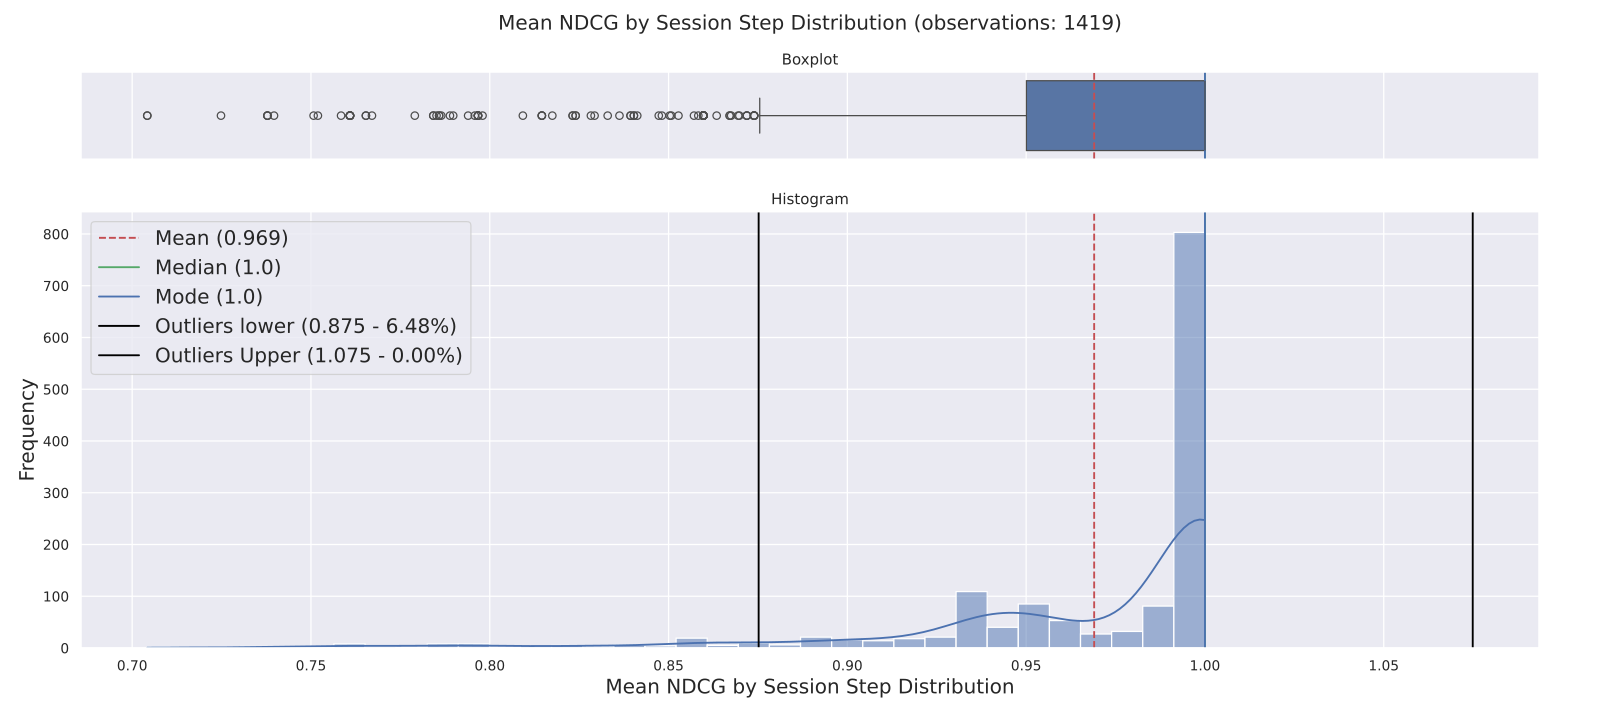
\includegraphics[width=15cm]{./images/llama2/mean_ndcg_by_session_step_distribution.png}
	\caption{En este gráfico se aprecia la media de \textit{Discounted cumulative gain} (\textit{NDCG}) por paso.}
	\label{fig:llama2-mean_ndcg_by_session_step_distribution}
\end{figure}

Para comenzar, se aprecia una distribución altamente sesgada. La mayoría de los valores de \textit{Discounted cumulative gain} (\textit{NDCG}) están concentrados cerca de $1.0$ (la moda y mediana son ambas $1.0$). Esto sugiere que, en general, el sistema de recomendación logra posicionar ítems relevantes en los primeros lugares de las listas, lo que es un indicador de buen desempeño. Hay una cantidad considerable de \textit{outliers} por debajo de $0.875$, representando aproximadamente el $6.48\%$ de los datos.
Estas sesiones podrían indicar casos en los que el sistema falla al generar recomendaciones relevantes.
La media de $0.969$ refleja un rendimiento global muy bueno. La mediana y moda, ambas iguales a $1.0$, refuerzan la idea de que una gran parte de las sesiones tienen un rendimiento ideal. El rango inter-cuartil (\textit{IQR}) es pequeño, lo que indica poca dispersión entre el $25\%$ y el $75\%$ de los datos, nuevamente señalando consistencia en el sistema.
En el histograma, se observa un pico pronunciado en $1.0$, mientras que los valores fuera de este rango son escasos. Esto confirma que la mayoría de las sesiones tienen un \textit{NDCG} óptimo o cercano a óptimo. Los valores más bajos aparecen de manera dispersa, pero su frecuencia es relativamente baja. A grandes rasgos, el sistema parece funcionar muy bien en términos de \textit{NDCG}, posicionando los ítems relevantes en los primeros lugares en la mayoría de las sesiones.
\clearpage


En la figura \ref{fig:llama2-mean_ndgc_by_session_step} se muestra la evolución de \textit{Discounted cumulative gain} (\textit{NDCG}) promedio por paso (\textit{Session Step}).

\begin{figure}[htbp]
	\centering
	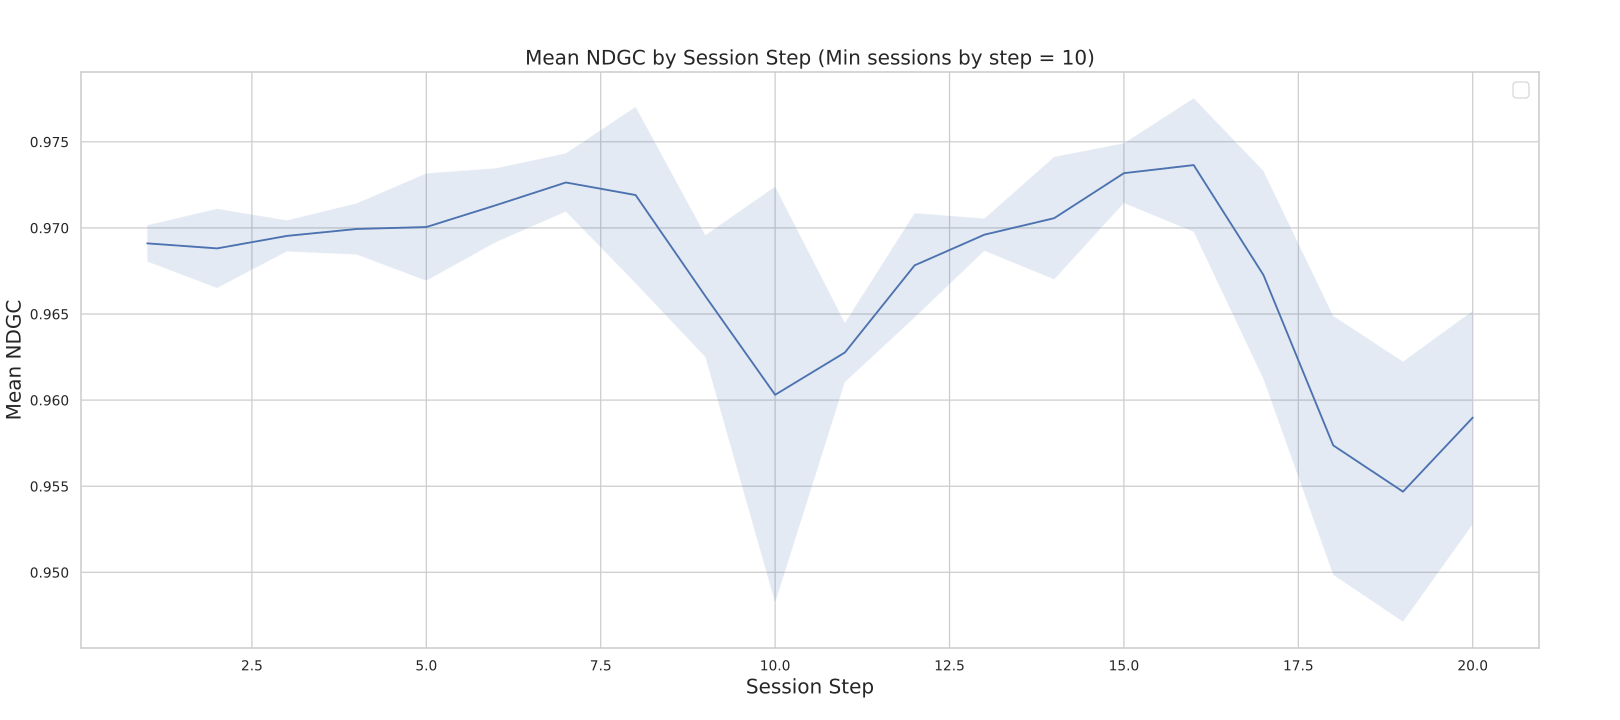
\includegraphics[width=15cm]{./images/llama2/mean_ndgc_by_session_step.png}
	\caption{En este gráfico se aprecia la evolución de \textit{Discounted cumulative gain} (\textit{NDCG}) promedio por paso(\textit{Session Step}).}
	\label{fig:llama2-mean_ndgc_by_session_step}
\end{figure}

El \textit{Discounted cumulative gain} (\textit{NDCG}) promedio se mantiene relativamente alto en todos los pasos de la sesión, con valores superiores a $0.95$, lo que demuestra un rendimiento consistente del sistema en términos de relevancia de las recomendaciones. Sin embargo, se observan fluctuaciones notables en ciertos pasos.
\newline
\newline
\newline
\textbf{Fluctuaciones principales}

\begin{itemize}
	\item \textbf{Incremento inicial}: Al principio (hasta el paso $5$), el \textit{NDCG} aumenta ligeramente, lo que sugiere que el sistema está afinando las recomendaciones en función de las primeras interacciones del usuario.
	\item \textbf{Descenso en el paso $10$}: Hay una caída pronunciada en el \textit{NDCG} promedio alrededor del paso $10$, alcanzando un valor cercano a $0.955$. Este descenso muestra el cambio entre las estrategias de recomendación basada en contenido versus basada en filtros colaborativos. Se aprecia que en promedio el \textit{NDCG} se recupera en $5$ pasos.
	\item \textbf{Variabilidad en pasos finales}: A partir del paso $15$, el \textit{NDCG} disminuye nuevamente, pero parece recuperarse ligeramente hacia el paso $20$. La amplitud del intervalo de confianza en estos pasos sugiere una mayor incertidumbre o dispersión en el rendimiento.

\end{itemize}


\textbf{Intervalos de confianza}

Los intervalos de confianza son más amplios en los pasos intermedios y finales (especialmente en los pasos $8-12$ y $17-20$), lo que indica mayor variabilidad en el rendimiento. Esto puede deberse a:

\begin{itemize}
	\item \textbf{Entre los pasos $8-12$}:
	      \begin{itemize}
		      \item Como ya se menciono, tenemos una baja debido al intercambio entre estrategias de recomendación.
		      \item Tal vez debería retrasarse el número de pasos en que se cambia la estrategia de recomendación. Este valor es un hiperparámetro a optimizar.
		      \item Se podría realizar un \textit{smooth} de ambas estrategias para minimizar la baja. Por ejemplo, seleccionando ambas estrategias intercaladas entre los pasos $8$ y $12$.
	      \end{itemize}
	\item \textbf{Entre los pasos $17-20$}:
	      \begin{itemize}
		      \item Usuarios con comportamientos menos predecibles en etapas avanzadas de la sesión.
		      \item Menor cantidad de datos para esos pasos (sesiones largas son menos comunes).
	      \end{itemize}
\end{itemize}

\clearpage

En la figura \ref{fig:llama2-mean_recall_by_session_step_distribution} se muestra el \textit{Recall} promedio por paso(\textit{Session Step}).

\begin{figure}[htbp]
	\centering
	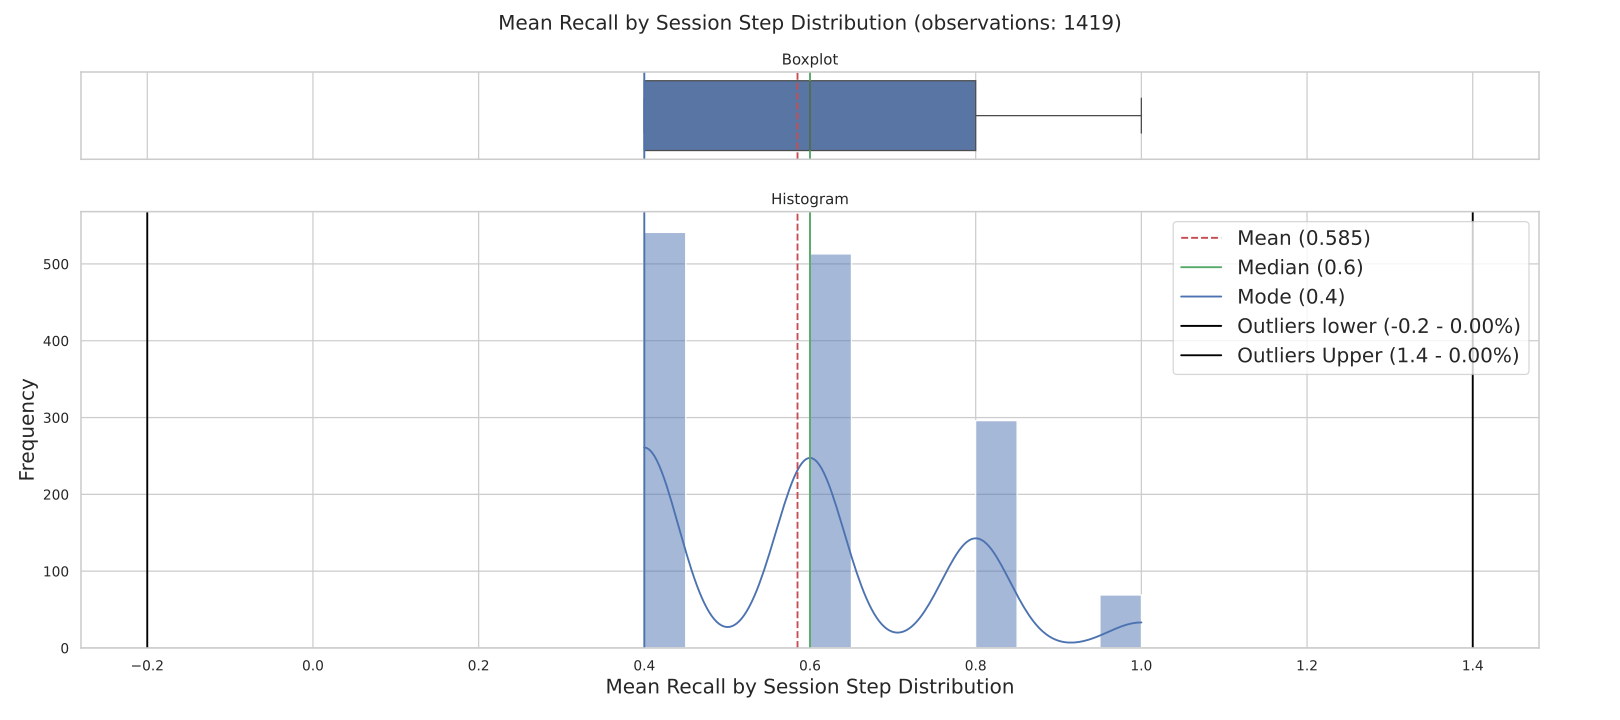
\includegraphics[width=15cm]{./images/llama2/mean_recall_by_session_step_distribution.png}
	\caption{En este gráfico se muestra el \textit{Recall} promedio por paso(\textit{Session Step})}
	\label{fig:llama2-mean_recall_by_session_step_distribution}
\end{figure}


La media y la mediana permanecen constantes, con un \textit{Recall} medio de $0.585$ y una mediana de $0.6$. La moda de $0.4$ refuerza que hay un grupo considerable de sesiones con desempeño más bajo. No se visualizan valores extremos significativos, con un rango ajustado entre $-0.2$ y $1.4$. La distribución refuerza la predominancia de valores alrededor de la mediana y un pequeño grupo de sesiones con \textit{Recall} más bajo.

En la figura \ref{fig:llama2-mean_recall_by_session_step_series} se muestra la evolución del \textit{Recall} promedio por paso(\textit{Session Step}).


\begin{figure}[htbp]
	\centering
	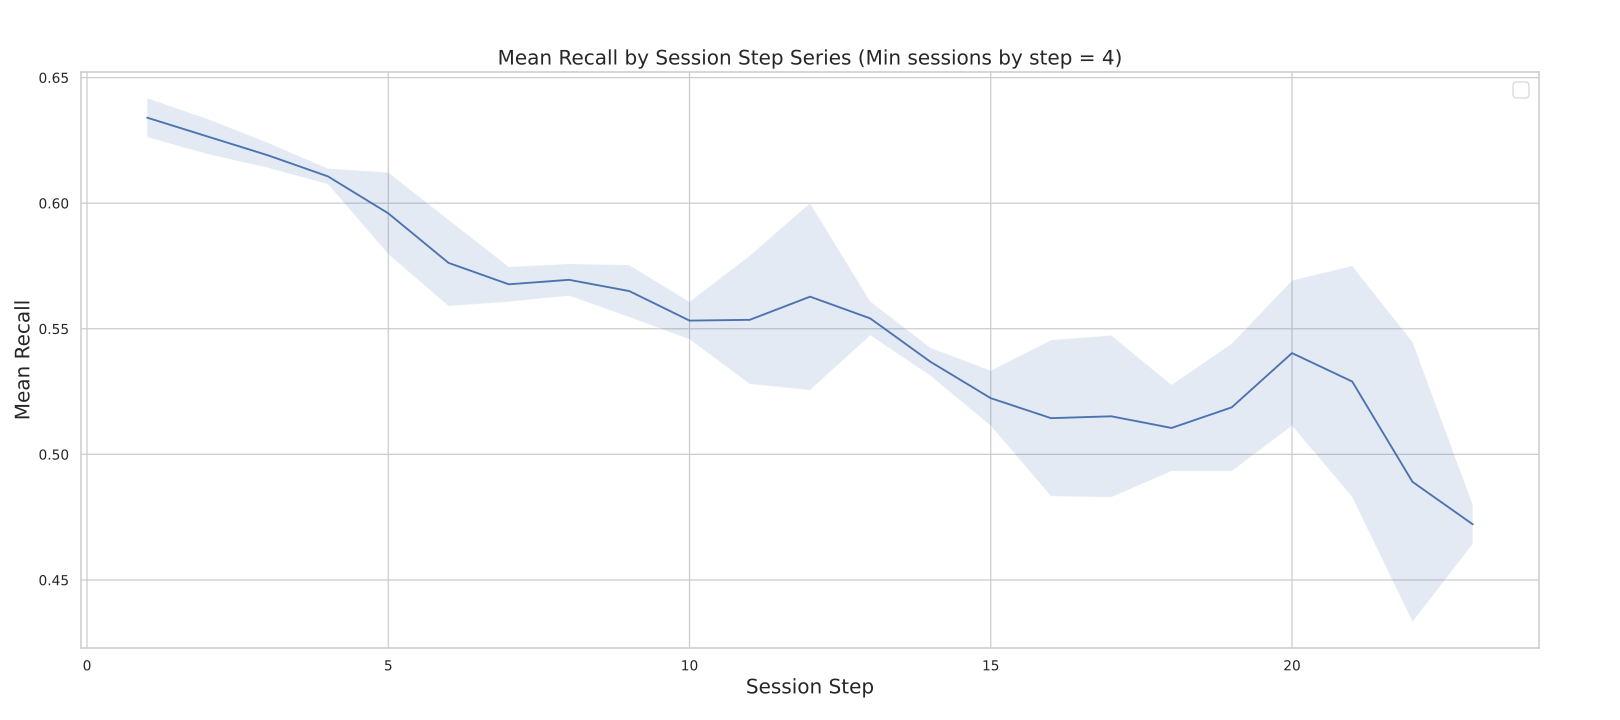
\includegraphics[width=15cm]{./images/llama2/mean_recall_by_session_step_series.png}
	\caption{En este gráfico se muestra la evolución del \textit{Recall} promedio por paso(\textit{Session Step}).}
	\label{fig:llama2-mean_recall_by_session_step_series}
\end{figure}

La tendencia muestra un descenso en el \textit{Recall} a medida que avanzan los pasos de sesión. El sistema enfrenta dificultades para mantener el desempeño en pasos superiores a $15$.
La incertidumbre del intervalo de confianza aumenta hacia los pasos finales debido a la menor cantidad de sesiones en esa etapa, algo esperado en distribuciones de series de tiempo. Esto sugiere que el sistema de recomendación tiene problema para retornar contenido relevante a medida que aumenta el número de pasos por sesión, ya sea por agotamiento de contenido popular o dificultad para realizar búsquedas detalladas. Por otro lado en parte podría deberse a una dificultad para realizar el \textit{ranking} personalizado.

En la figura \ref{fig:llama2-mean_reciprocal_rank_by_session_distribution} se muestra la distribución del \textit{Mean Reciprocal Rank (MRR)} por sesión.

\begin{figure}[htbp]
	\centering
	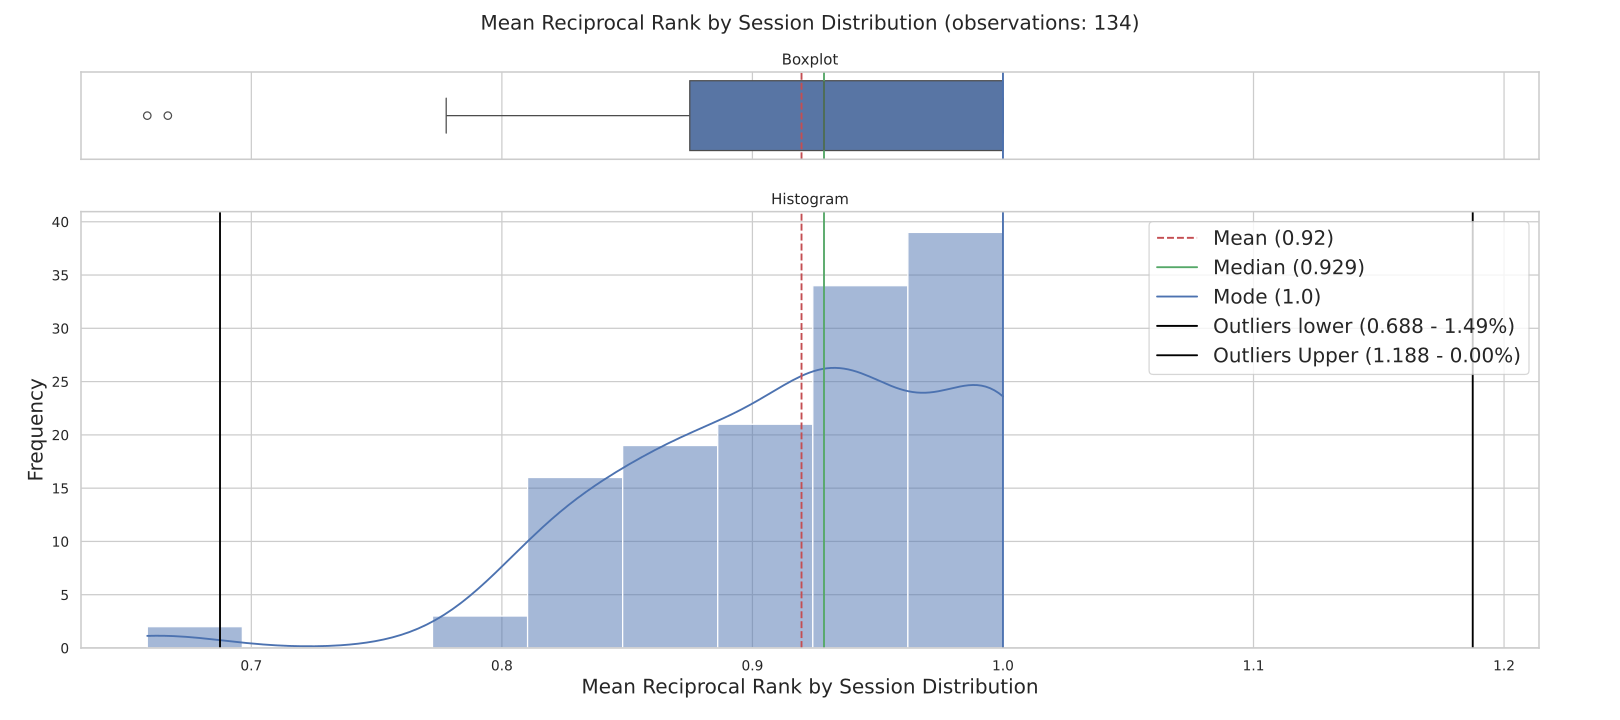
\includegraphics[width=15cm]{./images/llama2/mean_reciprocal_rank_by_session_distribution.png}
	\caption{En este gráfico se muestra
		la distribución del \textit{Mean Reciprocal Rank (MRR)} por sesión.}
	\label{fig:llama2-mean_reciprocal_rank_by_session_distribution}
\end{figure}

En la figura \ref{fig:llama2-mean_reciprocal_rank_by_session_distribution} se observa una distribución sesgada hacia la derecha, con valores de \textit{Mean Reciprocal Rank (MRR)} mayoritariamente altos. Una media de $0.92$, mediana de $0.929$ y finalmente una moda de $1.0$, indicando que muchas sesiones lograron la mejor calificación posible (la recomendación más relevante fue presentada en primer lugar). Por otro lado, existen algunos valores atípicos inferiores (menor a $0.688$), que representan aproximadamente el $1.49\%$ de las observaciones. Estas sesiones pueden haber tenido recomendaciones iniciales menos relevantes, lo que afectó negativamente al \textit{Mean Reciprocal Rank (MRR)}.

\clearpage

En la figura \ref{fig:llama2-mean_reciprocal_rank_by_session_step_series} muestra una serie con la evolución del \textit{Mean Reciprocal Rank (MRR)} por pasos de sesión.

\begin{figure}[htbp]
	\centering
	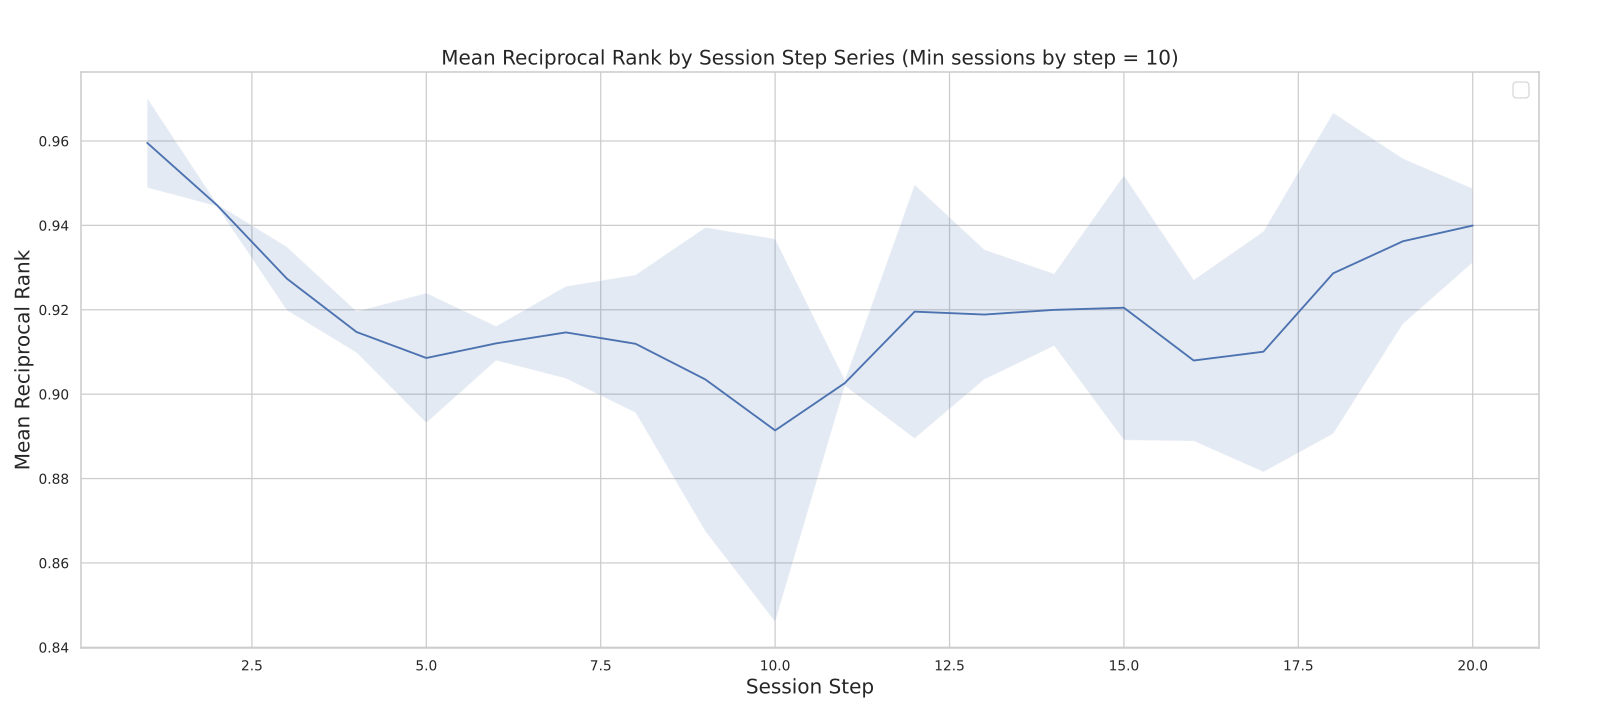
\includegraphics[width=15cm]{./images/llama2/mean_reciprocal_rank_by_session_step_series.png}
	\caption{Este gráfico muestra una serie con la evolución del \textit{Mean Reciprocal Rank (MRR)} por pasos de sesión.}
	\label{fig:llama2-mean_reciprocal_rank_by_session_step_series}
\end{figure}

El \textit{Mean Reciprocal Rank (MRR)} promedio comienza con valores altos en los primeros pasos (aproximadamente $0.96$), lo que sugiere un buen inicio en términos de calidad de recomendaciones. Sin embargo, se observa un descenso gradual hasta el paso $10$, donde alcanza su punto más bajo ($~0.88$). Después del paso $10$, vuelve a aumentar y se estabiliza cerca de $0.94$ en los pasos finales de la sesión.

Este comportamiento se debe al cambio en la estrategia de recomendación basada en contenido (utilizado en las primeras interacciones del usuario), a la estrategia basada en filtros colaborativos. En este caso, a diferencia de la evolución del \textit{NDGC}, la baja parece menos pronunciada. Los intervalos de confianza son amplios en los pasos intermedios y finales, indicando una variabilidad considerable del \textit{MRR} en esos puntos. De esta forma en pasos intermedios la variabilidad de debe al cambio de estrategia de recomendación, que produce que los mejores resultado no siempre se encuentren en las primeras posiciones. Hacia el final, la variabilidad puede deberse a un reducido numero de sesiones afectado por el \textit{leverage} o palanca de alguna sesión particular.


\clearpage

En la figura \ref{fig:llama2-rated_items_by_session_distribution} se puede visualizar la distribución de la cantidad de ítems relevantes calificados por sesión de usuario.

\begin{figure}[H]
	\centering
	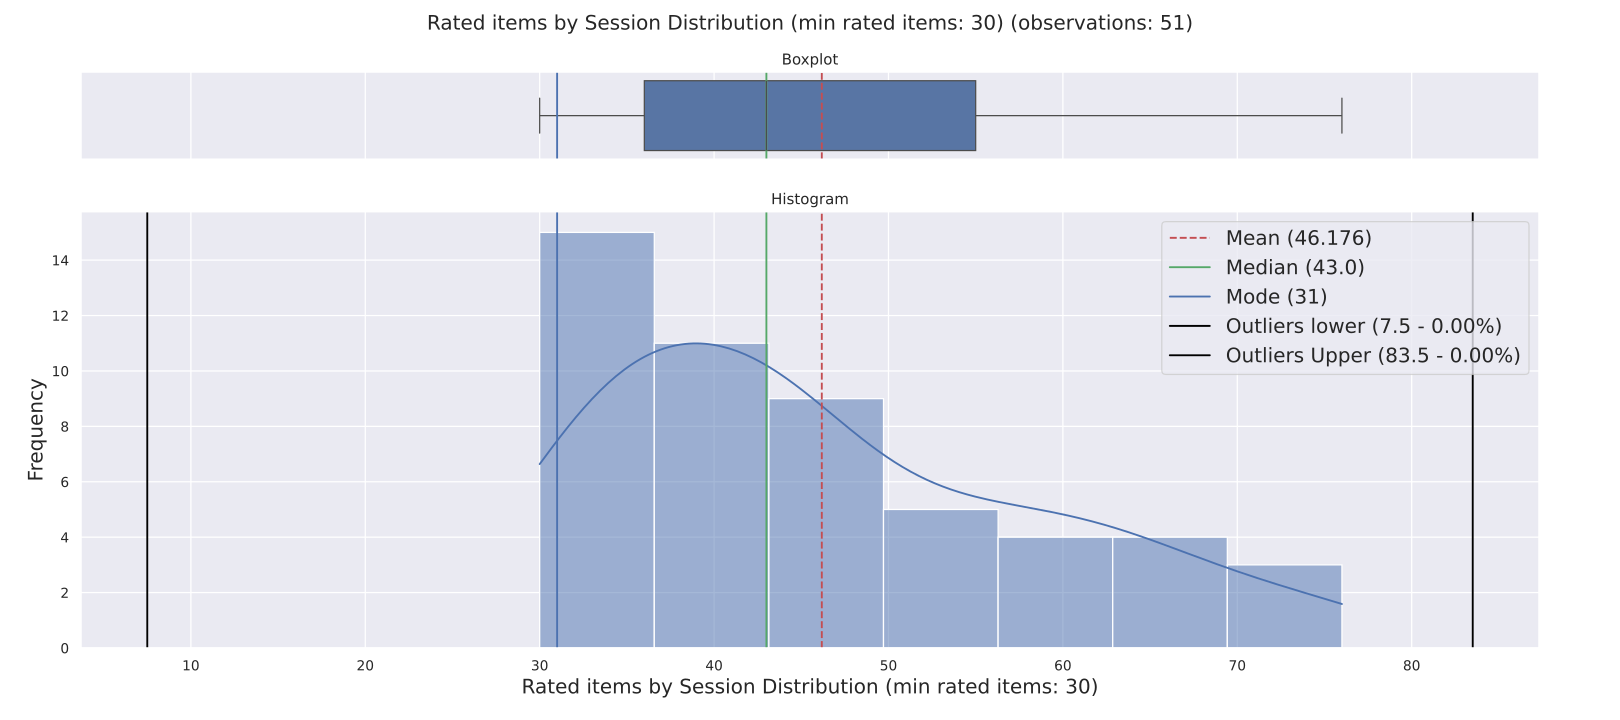
\includegraphics[width=15cm]{./images/llama2/rated_items_by_session_distribution.png}
	\caption{En este gráfico se puede visualizar la distribución de la cantidad de ítems relevantes calificados por sesión de usuario.}
	\label{fig:llama2-rated_items_by_session_distribution}
\end{figure}

En la figura \ref{fig:llama2-rated_items_by_session_distribution}  se aprecia  una distribución unimodal con asimetría positiva. La cola se extiende hacia la derecha y el pico principal se encuentra alrededor de los $30-35$ ítems. La densidad máxima está en el rango $25-45$ ítems.

\textbf{Interpretación por segmentos}

\begin{itemize}
	\item \textbf{Segmento medio ($30-45$ ítems)}: Concentra la mayoría de las sesiones. Representa el comportamiento típico de los usuarios. Sugiere un nivel de participación saludable del usuario.
	\item \textbf{Segmento alto ($45-80$ ítems)}: Cola larga con frecuencia decreciente. Representa sesiones extensas. Podría indicar usuarios muy comprometidos o experimentados.
\end{itemize}

La distribución sugiere que el sistema mantiene el interés del usuario durante un período considerable, siendo el rango más común entre $30-45$ ítems. La ausencia de \textit{outliers} indica un comportamiento bastante consistente entre usuarios.

\clearpage

En la figura \ref{fig:llama2-relevant_items_found_by_step_index_for_all_sessions} se muestra el número de ítems relevantes encontrados en cada paso para todas las sesiones de usuario, segmentado por la cantidad de ítems relevantes en las respuestas del sistemas de recomendación.

\begin{figure}[H]
	\centering
	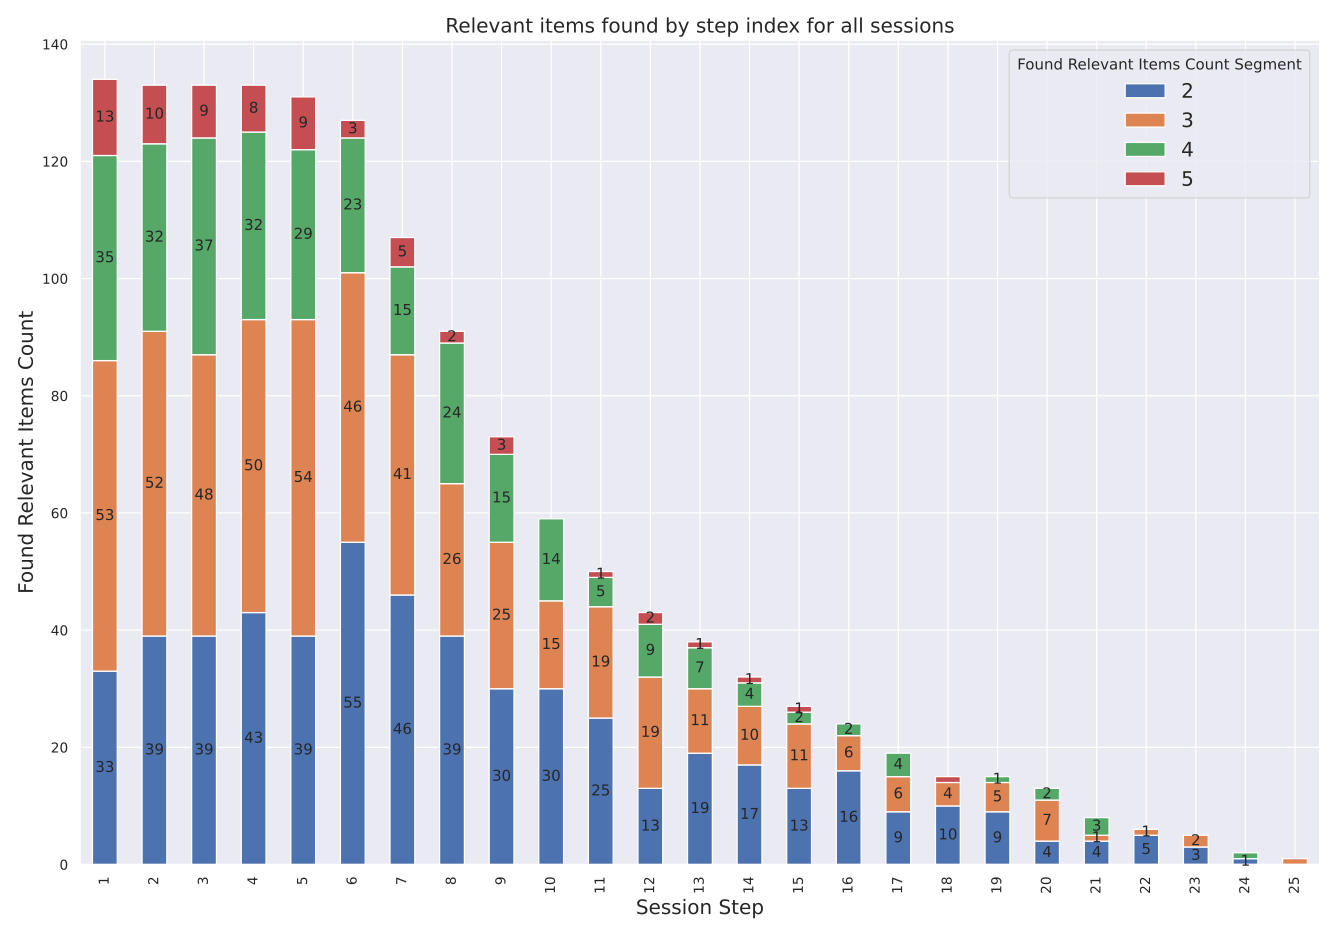
\includegraphics[width=15cm]{./images/llama2/relevant_items_found_by_step_index_for_all_sessions.png}
	\caption{En este gráfico se puede apreciar el número de ítems relevantes encontrados en cada paso para todas las sesiones de usuario, segmentado por la cantidad de ítems relevantes en las respuestas del sistemas de recomendación.}
	\label{fig:llama2-relevant_items_found_by_step_index_for_all_sessions}
\end{figure}

El número total de ítems encontrados disminuye gradualmente a medida que aumenta el numero de pasos de las sesiones. Los pasos iniciales tienen la mayor concentración de relevancia, lo que refleja un modelo más efectivo al inicio de las interacciones. Los segmentos para resultados con $2$ y $3$ ítems relevantes son dominantes a lo largo de todos los pasos.
Los segmentos para resultados con $4$ y $5$ ítems relevantes aparecen con mayor frecuencia en los pasos iniciales y desaparecen casi por completo hacia los pasos finales. A partir del paso $15$, la cantidad total de ítems relevantes es baja, con una tendencia a encontrar menos de $2$ ítems relevantes. Esto esta relacionado con la perdida de \textit{Recall} vista en la figura \ref{fig:llama2-mean_recall_by_session_step_series}, donde se aprecia que la perdida del \textit{Recall} a medida que aumenta el número de pasos por sesión. Claramente en sistema de recomendación tiene dificultades para encontrar contenido por nombre a medida que aumenta el número de pasos por sesión.

\chapter{Resultados utilizando el componente \textit{LLM} \textit{Llama3}}

En esta sección se presentan los resultados de la evaluación del sistema de recomendación utilizando el componente \textit{Llama3} para realizar el \textit{ranking} de ítems recomendados a un usuario.

En la figura \ref{fig:llama3-steps_count_by_session_distribution} se muestra la cantidad de pasos por sesión, donde un paso corresponde a una consulta realizada por un usuario.

\begin{figure}[H]
	\centering
	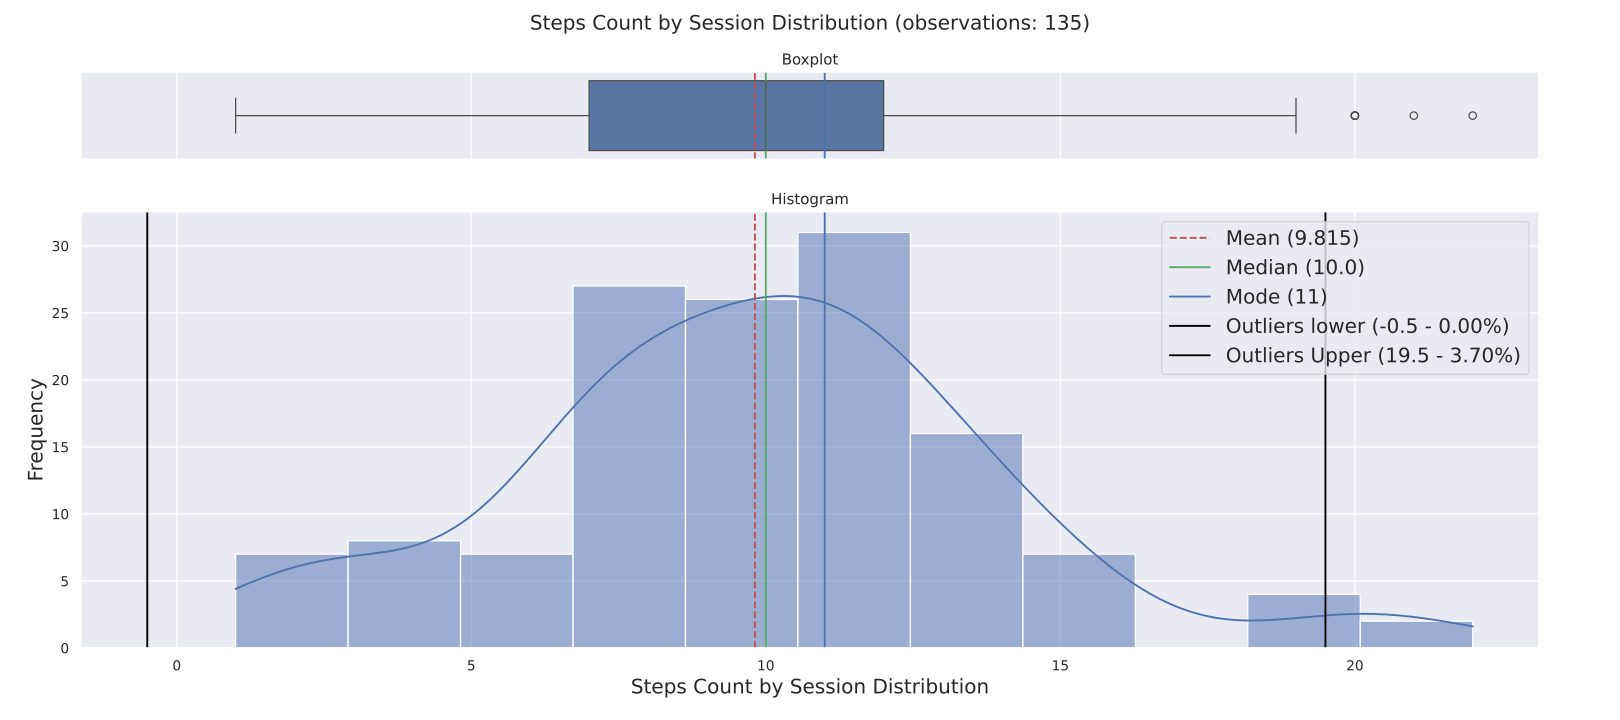
\includegraphics[width=15cm]{./images/llama3/steps_count_by_session_distribution.png}
	\caption{En el gráfico se aprecia la cantidad de pasos(consultas realizadas) por sesión de usuario.}
	\label{fig:llama3-steps_count_by_session_distribution}
\end{figure}

Se puede observar que la mayoría de las sesiones tienen una cantidad de pasos entre $7$ y $13$. Los valores atípicos superiores (\textit{outliers}) se encuentran por encima de $19$ pasos, representando el $3.7\%$ de las observaciones. La media se encuentra en $9.815$ pasos por sesión, mientra que la mediana esta en $10$ pasos, con una moda en $11$ pasos. La distribución es aproximadamente simétrica, con un leve sesgo hacia la izquierda, indicando que algunas sesiones terminan antes de alcanzar el promedio. Al utilizar el componente \textit{Llama2}, las sesiones tienen una cantidad promedio de pasos similar, pero la media y mediana muestran valores ligeramente más bajos, lo que sugiere que el sistema con \textit{Llama2} presenta interacciones más cortas en promedio. Utilizando \textit{Llama3} parece que se generan sesiones con una mayor dispersión en su cantidad de pasos (más amplitud en el \textit{boxplot}) y más sesiones con pasos largos (evidenciado por más \textit{outliers} superiores en este caso). El histograma con \textit{Llama2} tiene una concentración más marcada alrededor de $7-10$ pasos, mientras que en \textit{Llama3} se observa una tendencia a extenderse más hacia los pasos superiores ($10-15$). Con \textit{Llama3} hay un mayor porcentaje de sesiones con pasos fuera de lo esperado ($3.7\%$ por encima de $19$), lo que puede indicar que este modelo tiende a mantener sesiones más largas para ciertos usuarios o escenarios específicos.

\clearpage

En la figura \ref{fig:llama3-sessions_count_by_session_step} se muestra el número de sesiones que realizaron consultas a lo largo de la secuencia de pasos definida por todas las sesiones generadas durante la prueba de evaluación.

\begin{figure}[H]
	\centering
	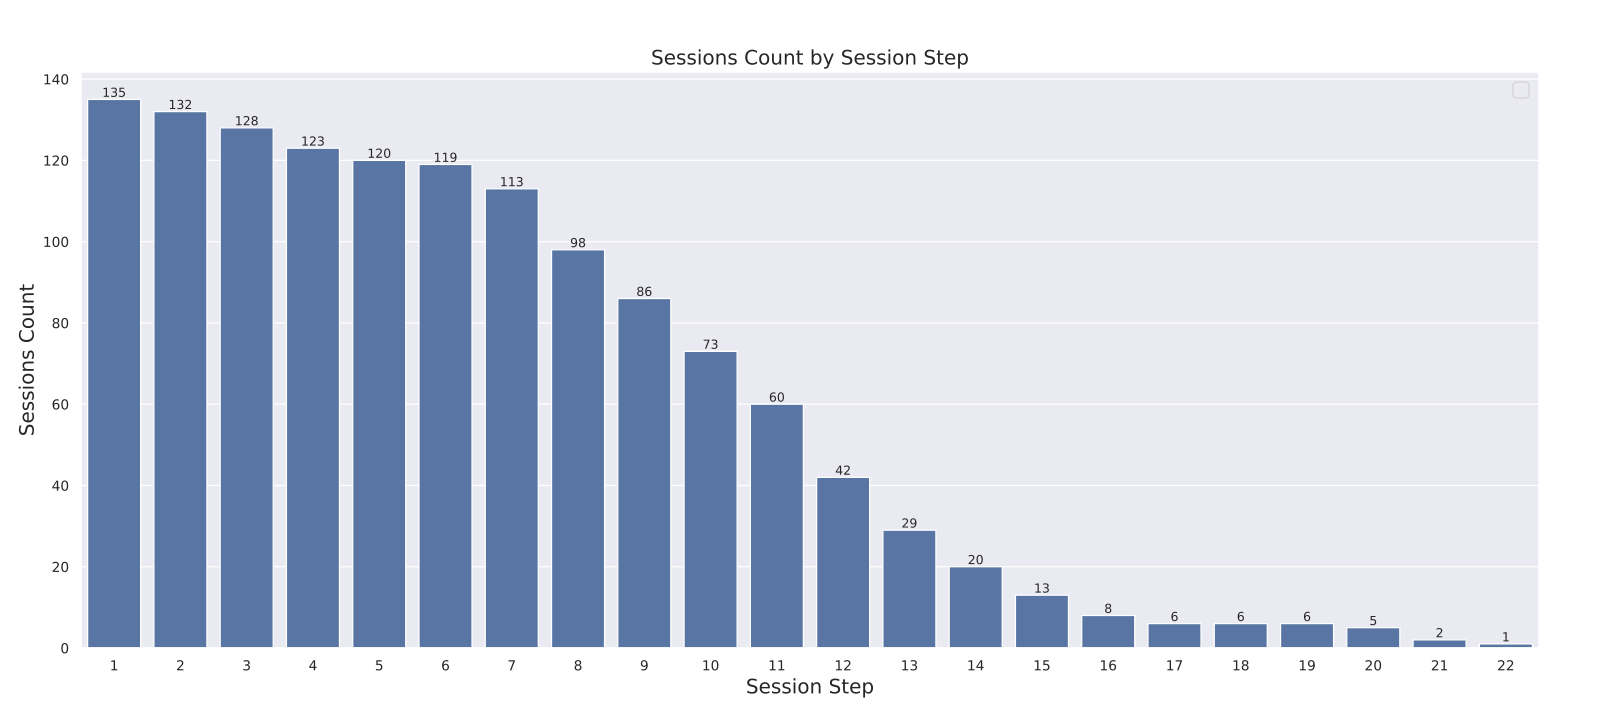
\includegraphics[width=15cm]{./images/llama3/sessions_count_by_session_step.png}
	\caption{En este gráfico se aprecia el número de sesiones que realizaron consultas a lo largo de la secuencia de pasos definida por todas las sesiones generadas durante la prueba de evaluación.}
	\label{fig:llama3-sessions_count_by_session_step}
\end{figure}

El mayor número de sesiones se concentra en los primeros pasos: $135$ sesiones en el primer paso, $132$ en el segundo, con un decrecimiento constante a medida que aumenta el número de pasos. A partir del paso $9$, la cantidad de sesiones disminuye más significativamente, llegando a $1$ sola sesión en el paso $22$. La tendencia muestra que la mayoría de las sesiones terminan antes del paso $10$. Esto es coherente con una interacción eficiente donde los usuarios obtienen resultados relevantes en los primeros intentos.
Existen sesiones que persisten mas allá de los $20$ pasos, aunque son minoritarias. Esto indica posibles escenarios donde el modelo no logra satisfacer la necesidad del usuario rápidamente. Con \textit{Llama2}, el conteo de sesiones por paso también disminuye progresivamente, pero el número de sesiones que persisten después del paso $10$ son menos en comparación con \textit{Llama3}. Esto sugiere que \textit{Llama3} puede estar generando más recomendaciones en pasos posteriores, aumentando la duración de ciertas sesiones. \textit{Llama3} tiene una mayor proporción de sesiones extendidas (más de $15$ pasos). Esto podría deberse a un diseño que busca explorar más alternativas antes de finalizar una sesión o a una dificultad en encontrar contenido relevante en los primeros pasos. En los primeros $5$ pasos, ambos modelos parecen manejar un volumen similar de sesiones. Sin embargo, \textit{Llama2} muestra una mayor proporción de sesiones finalizadas dentro de este rango, indicando una mayor eficiencia en cerrar interacciones rápidamente.

\clearpage

En la figura \ref{fig:llama3-found_items_count_by_session_step_distribution} se muestra la cantidad de ítems relevantes encontrados en cada respuesta del modelo de recomendación. Un ítem relevante es aquel que cuenta con una calificación del usuario en el conjunto de evaluación. Por lo tanto, si el sistema retorna un ítem que no está en la consulta, consideramos que no es relevante.


\begin{figure}[H]
	\centering
	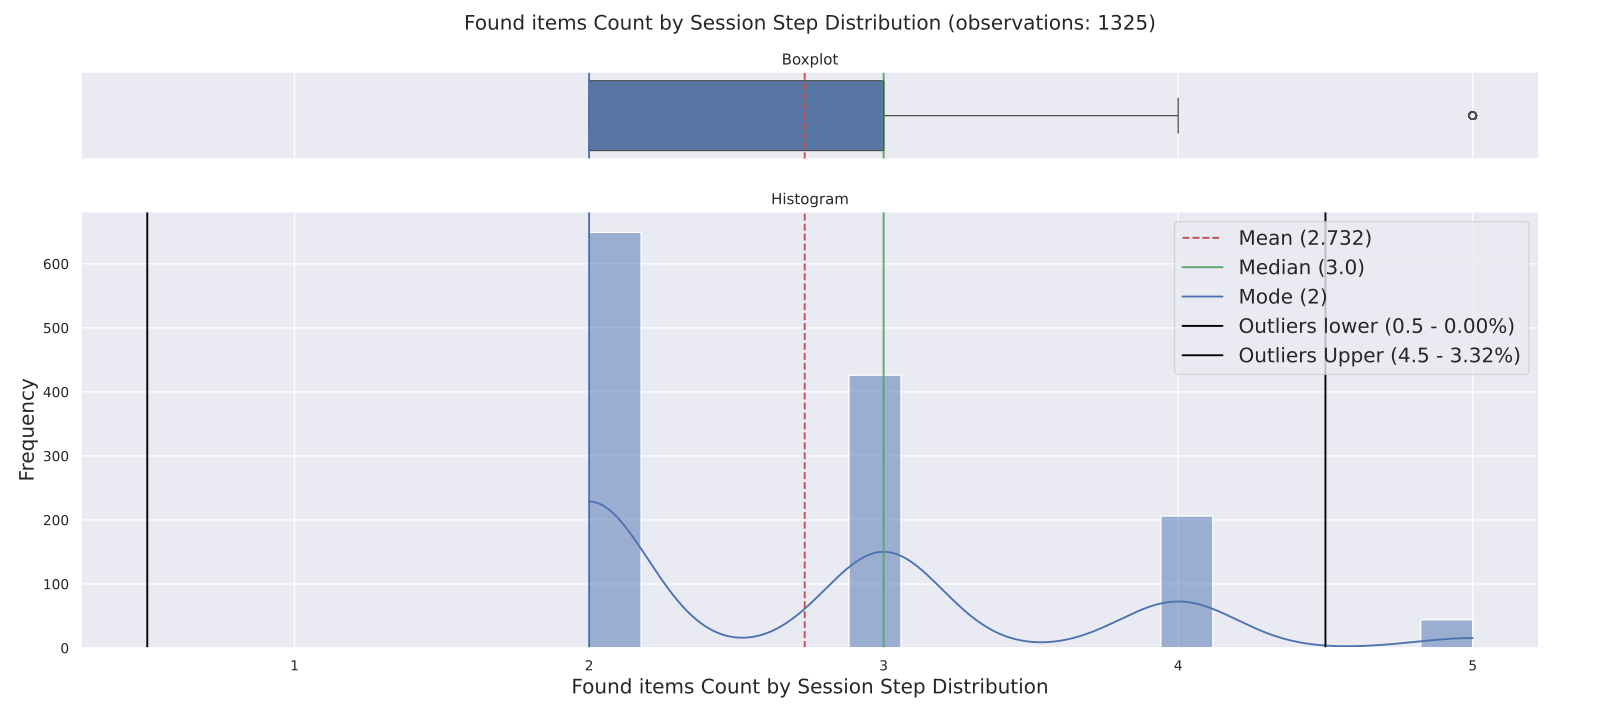
\includegraphics[width=15cm]{./images/llama3/found_items_count_by_session_step_distribution.png}
	\caption{En el gráfico se aprecia la cantidad de ítems relevantes encontrado en cada respuesta del modelo de recomendación}
	\label{fig:llama3-found_items_count_by_session_step_distribution}
\end{figure}

La mediana de $3$ indicando que en la mayoría de los pasos de sesión se encuentran $3$ ítems relevantes. La moda de $2$, el número más frecuente de ítems relevantes encontrados por paso. Existe un pequeño porcentaje de valores atípicos ($3.32\%$) de pasos en los que se encuentran más de $4.5$ ítems relevantes, lo que representa situaciones excepcionales. El histograma muestra una clara concentración en $2$ y $3$ ítems relevantes encontrados, con una rápida caída de frecuencias para valores superiores. El \textit{boxplot} refuerza esta observación, con un rango inter-cuartílico ajustado entre $2$ y $3.5$ ítems relevantes encontrados. Aunque minoritaria, hay una pequeña proporción de pasos de sesión donde se encuentran más de $4$ ítems relevantes.
Al utilizar \textit{Llama2}, la media es ligeramente inferior, cercana a $2.5$. Esto sugiere que \textit{Llama3} tiene un mejor rendimiento en términos de la cantidad de items relevantes encontrados por paso. Ambos modelos comparten una moda de $2$ ítems, pero \textit{Llama3} muestra una mediana más alta ($3$ frente a $2.5$ en \textit{Llama2}). Esto indica que el modelo más nuevo tiene un comportamiento más consistente para encontrar más ítems relevantes.
Con \textit{Llama2}, los pasos donde se encuentran más de $4$ ítems relevantes son aún menos frecuentes, lo que indica que \textit{Llama3} ha mejorado en identificar un mayor número de recomendaciones útiles en casos excepcionales.

\clearpage

En la figura \ref{fig:llama3-mean_average_precision_by_session_distribution} se muestra la distribución de la métrica \textit{Mean Average Precision}(\textit{MAP}) por sesión de usuario.

\begin{figure}[H]
	\centering
	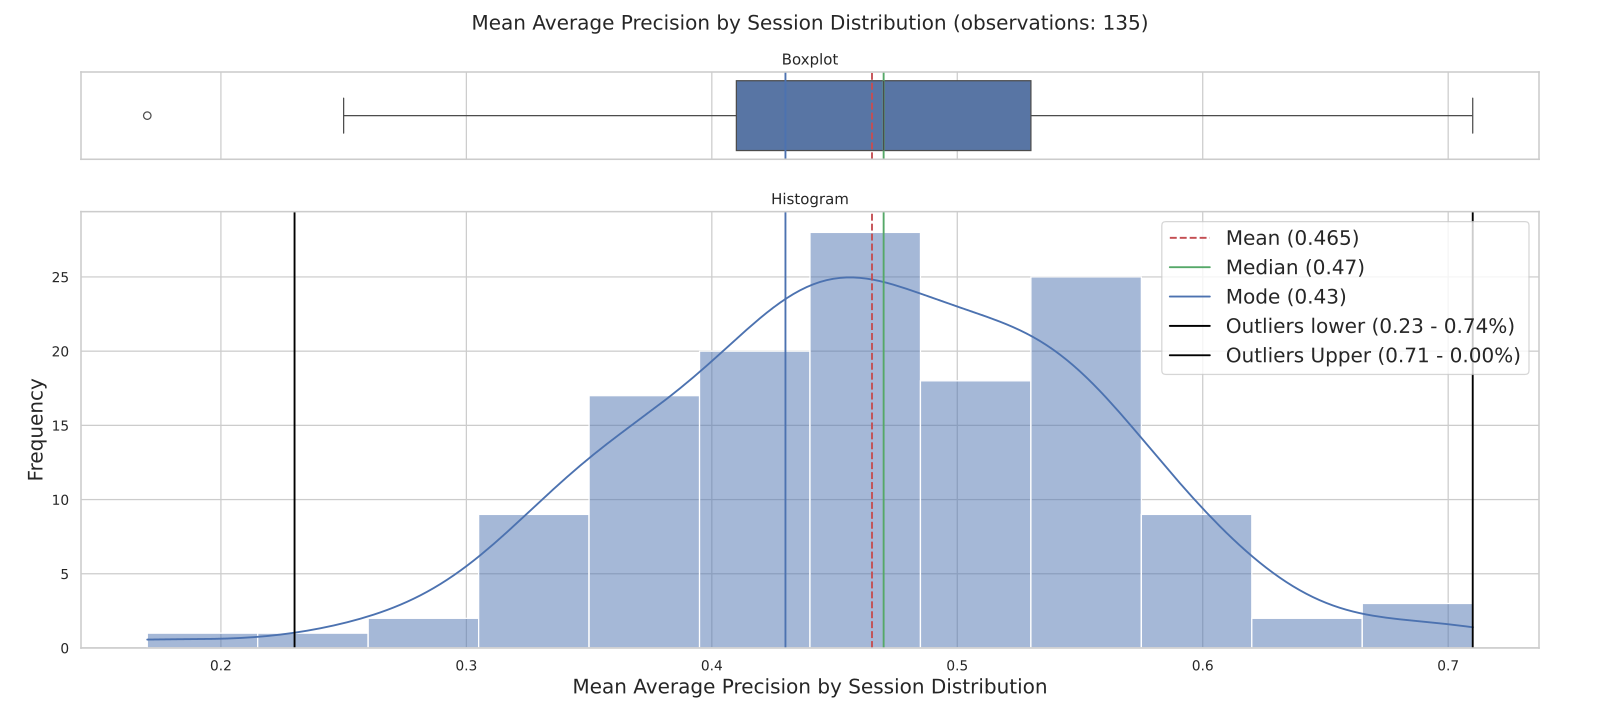
\includegraphics[width=15cm]{./images/llama3/mean_average_precision_by_session_distribution.png}
	\caption{En este gráfico se muestra la distribución de la métrica \textit{Mean Average Precision}(\textit{MAP}) por sesión de usuario.}
	\label{fig:llama3-mean_average_precision_by_session_distribution}
\end{figure}

El modelo presenta una precisión media de $0.465$ ($46.5\%$), con una mediana de $0.47$ ($47\%$) y una moda de $0.43$ ($43\%$). Esta dispersión entre las medidas de tendencia central sugiere una distribución con cierta asimetría. La forma del histograma revela una distribución más aplanada indicando variabilidad en el rendimiento del sistema.

El rango de valores se extiende desde aproximadamente $0.2$ hasta $0.7$, mostrando una amplitud considerable en la precisión de las recomendaciones. Hay presencia de valores atípicos, con \textit{outliers} inferiores a $0.23$ ($0.74\%$ de las observaciones), lo que indica casos ocasionales de rendimiento significativamente bajo. La distribución muestra una concentración importante de observaciones en el rango de $0.4$ a $0.5$, pero también presenta una dispersión considerable hacia ambos extremos. Esta característica sugiere que el sistema, aunque funcional, muestra variabilidad en su capacidad de generar recomendaciones precisas. Al contrastar estos resultados con el sistema basado en \textit{Llama2}, emergen diferencias significativas: \textit{Llama3} muestra una precisión media ($0.465$) significativamente menor que \textit{Llama 2} ($0.548$). La diferencia de $8.3$ puntos porcentuales representa una brecha considerable en eficacia. \textit{Llama 3} exhibe mayor variabilidad en sus predicciones, evidenciada por su distribución más dispersa. La presencia de múltiples picos contrasta con la distribución más uniforme de \textit{Llama 2}. Los valores atípicos son más frecuentes en \textit{Llama 3}, especialmente en el rango inferior. \textit{Llama 3} opera en un rango más amplio ($0.2-0.7$) comparado con \textit{Llama 2} ($0.4-0.8$). La concentración de valores en rangos más bajos sugiere un rendimiento general inferior. La mayor dispersión en las medidas de tendencia central de \textit{Llama 3} indica menor confiabilidad. Ademas, la presencia de valores extremos más frecuentes sugiere mayor interpretabilidad en las recomendaciones. Las diferencias expuestas hasta el momento sugieren que, la versión del sistema de recomendación que utiliza \textit{Llama3} presenta desafíos significativos en términos de consistencia y precisión cuando se compara con el modelo que utiliza \textit{Llama2}. La mayor variabilidad y menor precisión media indican que podría requerir ajustes o mejoras adicionales para alcanzar el nivel de rendimiento mostrado por el modelo con \textit{Llama2}.

\clearpage

En la figura \ref{fig:llama3-mean_average_precision_by_session_step_series} se muestra la evolución de la media de \textit{Mean Average Precision}(\textit{MAP}) por paso.

\begin{figure}[H]
	\centering
	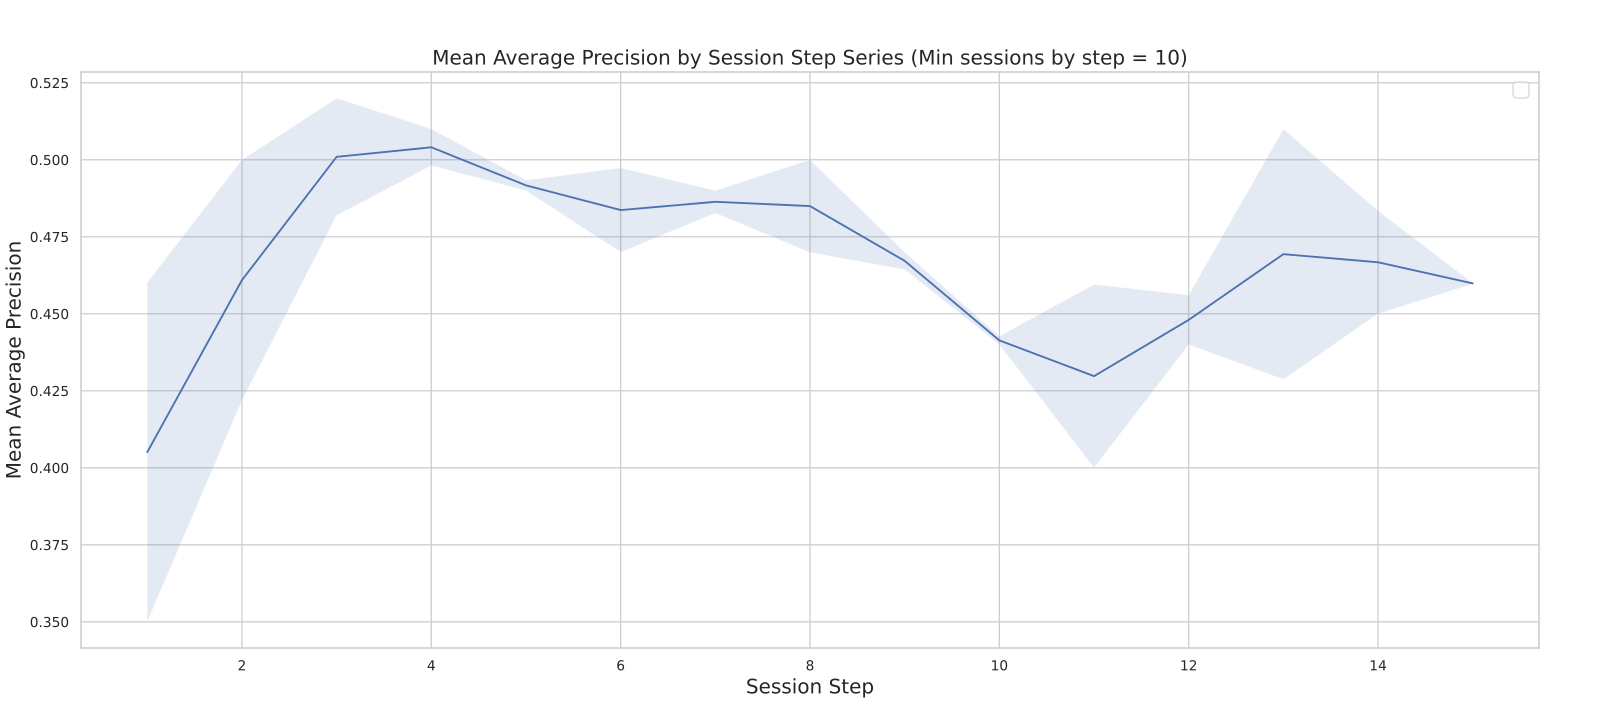
\includegraphics[width=15cm]{./images/llama3/mean_average_precision_by_session_step_series.png}
	\caption{En este gráfico se muestra la evolución la media de \textit{Mean Average Precision}(\textit{MAP}) por paso.}
	\label{fig:llama3-mean_average_precision_by_session_step_series}
\end{figure}

Se observa un patrón distintivo en su comportamiento a lo largo de las sesiones. El modelo inicia con un rendimiento relativamente bajo, aproximadamente en $0.35$, pero muestra una notable capacidad de adaptación durante las primeras sesiones. Esta fase inicial de aprendizaje rápido se caracteriza por un incremento pronunciado en el rendimiento hasta alcanzar un punto máximo alrededor del paso $5$, donde la precisión se estabiliza cerca de $0.50$.

Tras alcanzar su pico de rendimiento, el modelo mantiene una relativa consistencia en sus predicciones durante las sesiones intermedias ($5-8$), aunque se observa una ligera tendencia descendente. Las últimas sesiones presentan oscilaciones más significativas, sugiriendo cierta inestabilidad en el rendimiento a largo plazo. El intervalo de confianza muestra una mayor incertidumbre tanto en las sesiones iniciales como en las finales, con un período de mayor estabilidad en las sesiones intermedias.

La comparación al utilizar ambos componentes(\textit{Llama 3} y \textit{Llama 2}) revela patrones casi opuestos en su evolución temporal. Mientras que el modelo con \textit{Llama2} exhibe una degradación gradual desde un punto inicial alto, el modelo con \textit{Llama 3} muestra una mejora significativa desde un punto inicial bajo, seguida de una mayor estabilidad. Esta diferencia fundamental en sus comportamientos sugiere distintas fortalezas y casos de uso óptimos para cada modelo.

Resulta particularmente interesante observar cómo ambos modelos tienden a converger a niveles similares de rendimiento hacia el final de las sesiones, aunque llegan a este punto por caminos muy diferentes. Fuera de la diferencias en la evolución del \textit{MAP}, \textit{Llama2} se mantiene desde el inicio con valores de por encima de \textit{Llama3} a pesar de converger a valores similares hacia el final de la serie.


\clearpage


En la figura \ref{fig:llama3-mean_ndcg_by_session_step_distribution} se muestra la distribución de la métrica \textit{Normalized Discounted Cumulative Gain (NDCG)} por paso.

\begin{figure}[H]
	\centering
	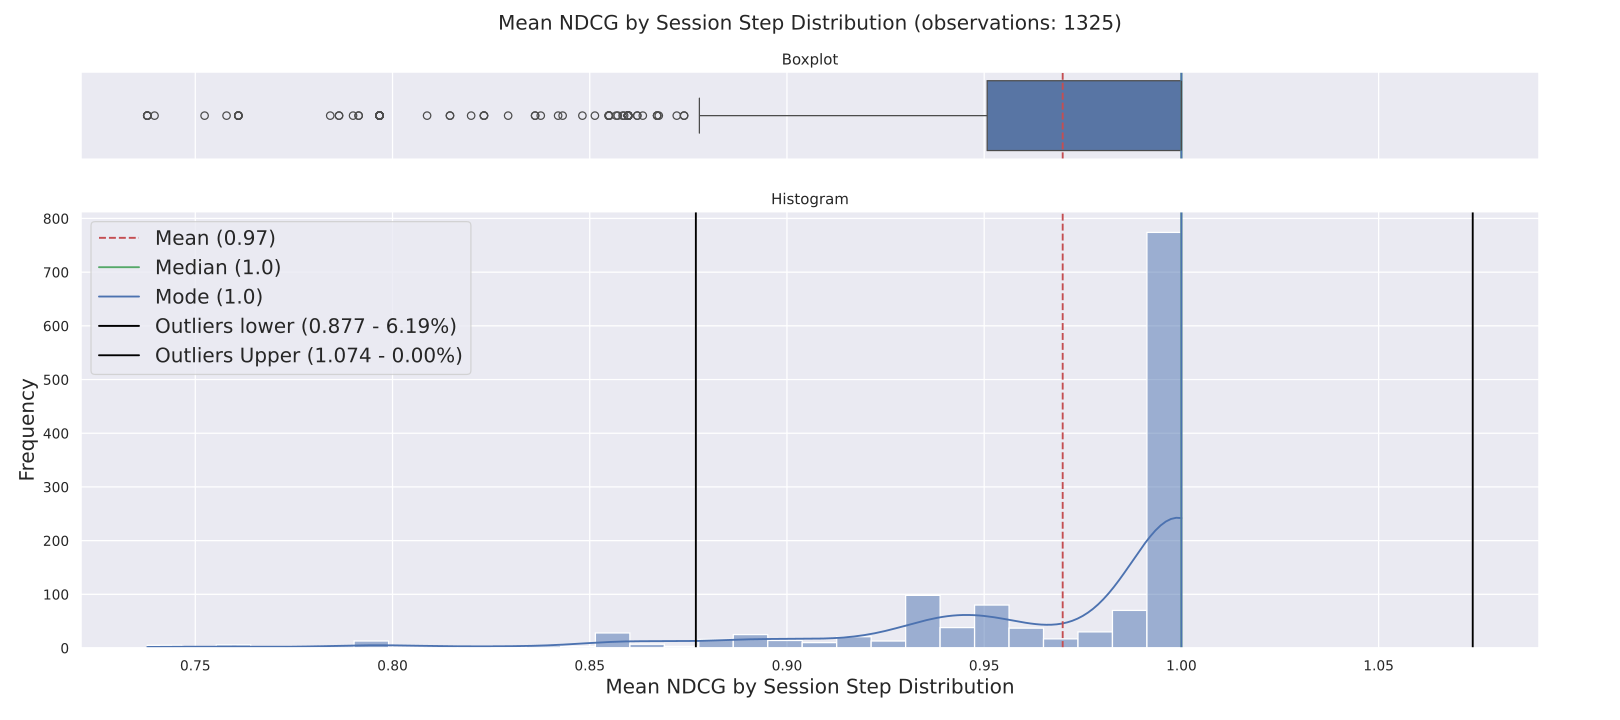
\includegraphics[width=15cm]{./images/llama3/mean_ndcg_by_session_step_distribution.png}
	\caption{Este gráfico describe la distribución de la métrica \textit{Normalized Discounted Cumulative Gain (NDCG)}  por paso.
	}
	\label{fig:llama3-mean_ndcg_by_session_step_distribution}
\end{figure}

El gráfico de la figura \ref{fig:llama3-mean_ndcg_by_session_step_distribution} muestra la distribución del \textit{Normalized Discounted Cumulative Gain (NDCG)} por paso basada en $1325$ observaciones. La distribución presenta características notables: una media de $0.97$, con la mediana y moda coincidiendo en $1.0$, lo que indica un sesgo significativo hacia valores óptimos en el rendimiento del sistema de recomendación.
El histograma revela una estructura marcadamente asimétrica, donde se destaca un pico prominente en el valor $1.0$, que concentra aproximadamente $750$ observaciones. Esta característica sugiere que una proporción mayoritaria de las sesiones alcanza un rendimiento óptimo en términos de posicionamiento de recomendaciones relevantes. La distribución muestra una cola izquierda que se extiende hacia valores más bajos, con una concentración significativa de observaciones en el rango entre $0.95$ y $1.0$.
En cuanto a los casos atípicos, se presenta un $6.19\%$ de \textit{outliers} por debajo de $0.877$, mientras que no se observan \textit{outliers} a derecha. El \textit{boxplot} muestra una distribución compacta en el rango inter-cuartil, lo que indica una alta consistencia en el rendimiento del sistema para la mayoría de las sesiones.
Al comparar estos resultados con \textit{LLama2}, se observan algunas diferencias interesantes. \textit{LLama2} cuenta con un mayor número de observaciones ($1419$) y presenta una media ligeramente inferior ($0.969$). La proporción de \textit{outliers} en \textit{LLama2} es mayor ($6.48\%$) y su límite inferior es más bajo ($0.875$). Esta comparación sugiere que \textit{LLama3} logra un manejo más eficiente de los casos problemáticos, aunque mantiene un patrón de distribución similar al de su predecesor.
La evolución de \textit{LLama2} a \textit{LLama3} muestra una mejora sutil pero consistente en el manejo de casos atípicos, manteniendo al mismo tiempo la robustez general del sistema de recomendación. Aunque las diferencias no son dramáticas, indican una optimización en el tratamiento de sesiones que podrían presentar desafíos particulares, como perfiles de usuario atípicos o casos con datos problemáticos.

\clearpage

En la figura \ref{fig:llama3-mean_ndgc_by_session_step} se muestra la evolución de \textit{Discounted cumulative gain (NDCG)} promedio por paso (\textit{Session Step}).

\begin{figure}[H]
	\centering
	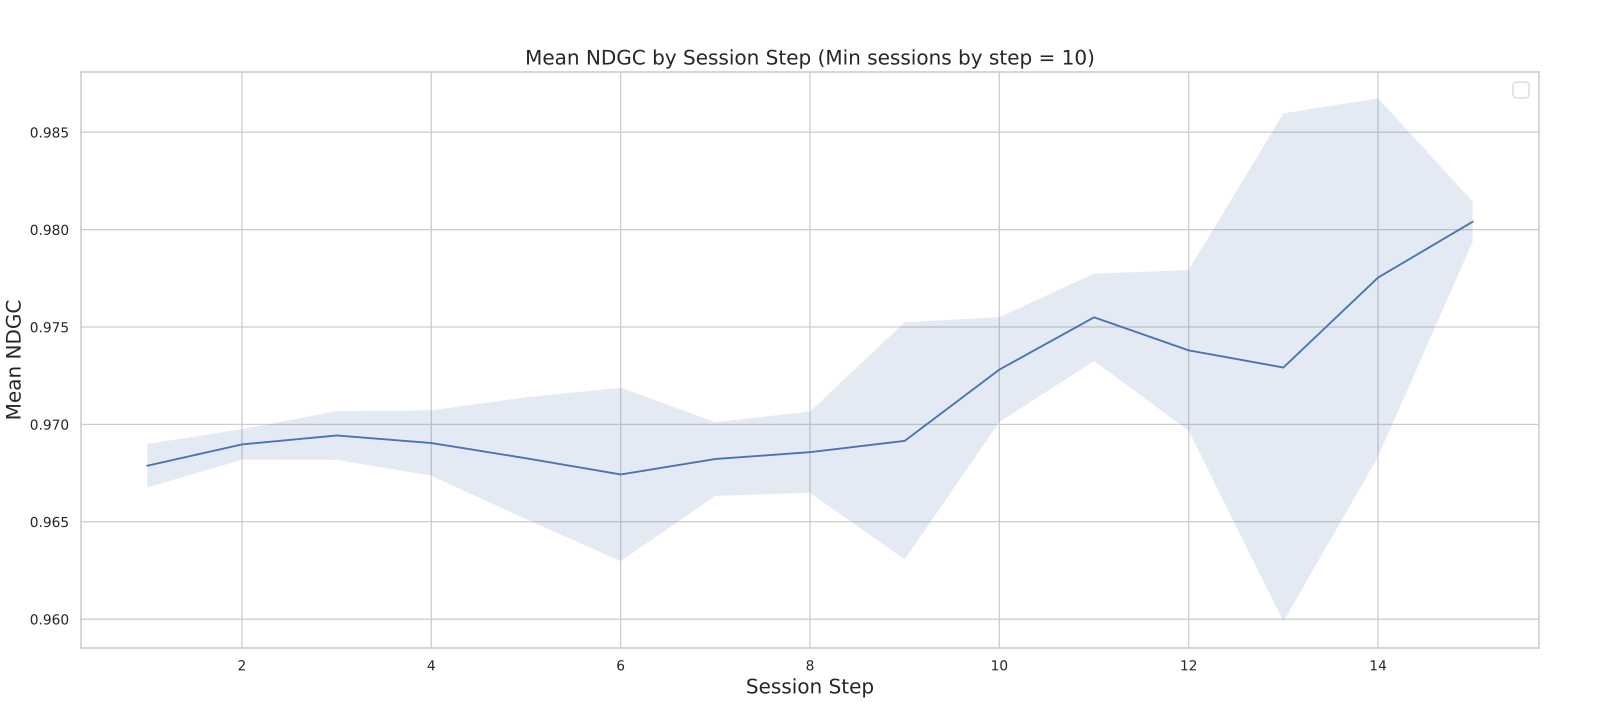
\includegraphics[width=15cm]{./images/llama3/mean_ndgc_by_session_step.png}
	\caption{Este gráfico se muestra la evolución de \textit{Discounted cumulative gain (NDCG)} promedio por paso (\textit{Session Step}).}
	\label{fig:llama3-mean_ndgc_by_session_step}
\end{figure}

En la figura \ref{fig:llama3-mean_ndgc_by_session_step} se muestra la evolución del \textit{Discounted cumulative gain (NDCG)}, la cual tiene un patrón notablemente diferente a la medición recabada utilizando el componente \textit{Llama2} (figura \ref{fig:llama2-mean_ndgc_by_session_step}). El gráfico presenta una tendencia general ascendente más estable, comenzando desde aproximadamente $0.965$ y alcanzando valores cercanos a $0.98$ hacia el final de la sesión. No se observa la pronunciada caída que caracteriza a \textit{LLama2} en el paso $10$, lo que sugiere una mejor integración entre las diferentes estrategias de recomendación.
Las diferencias más notables entre ambos modelos son:

Al utilizar \textit{LLama3} muestra una mayor estabilidad general, con fluctuaciones menos pronunciadas que \textit{LLama2}. Esto sugiere una mejor gestión en la transición entre diferentes estrategias de recomendación. Mientras que al utilizar \textit{LLama2} muestra una tendencia descendente en los pasos finales, \textit{LLama3} mantiene una tendencia ascendente, indicando una mejor capacidad para mantener la calidad de las recomendaciones en sesiones más largas. \textit{LLama3} presenta intervalos de confianza más amplios hacia el final de la sesión, pero sin la marcada variabilidad que muestra \textit{LLama2} en los pasos $8-12$ y $17-20$.
\textit{LLama3} parece manejar mejor las sesiones largas, mostrando incluso una mejora en el rendimiento, a diferencia de la degradación observada en \textit{LLama2}.

Estas diferencias sugieren que al utilizar \textit{LLama3} el sistema de recomendación representa una mejora significativa en términos de estabilidad y consistencia en el \textit{Discounted cumulative gain (NDCG)} promedio, especialmente en el manejo de sesiones largas y en la transición entre diferentes estrategias de recomendación. La eliminación de la caída pronunciada en el paso $10$ y la tendencia ascendente en los pasos finales indican una mejor adaptación a los patrones de comportamiento del usuario y una mayor robustez en el manejo de casos diversos.


\clearpage

En la figura \ref{fig:llama3-mean_recall_by_session_step_distribution} se muestra la distribución del \textit{Recall} promedio por paso (\textit{Session Step}).


\begin{figure}[H]
	\centering
	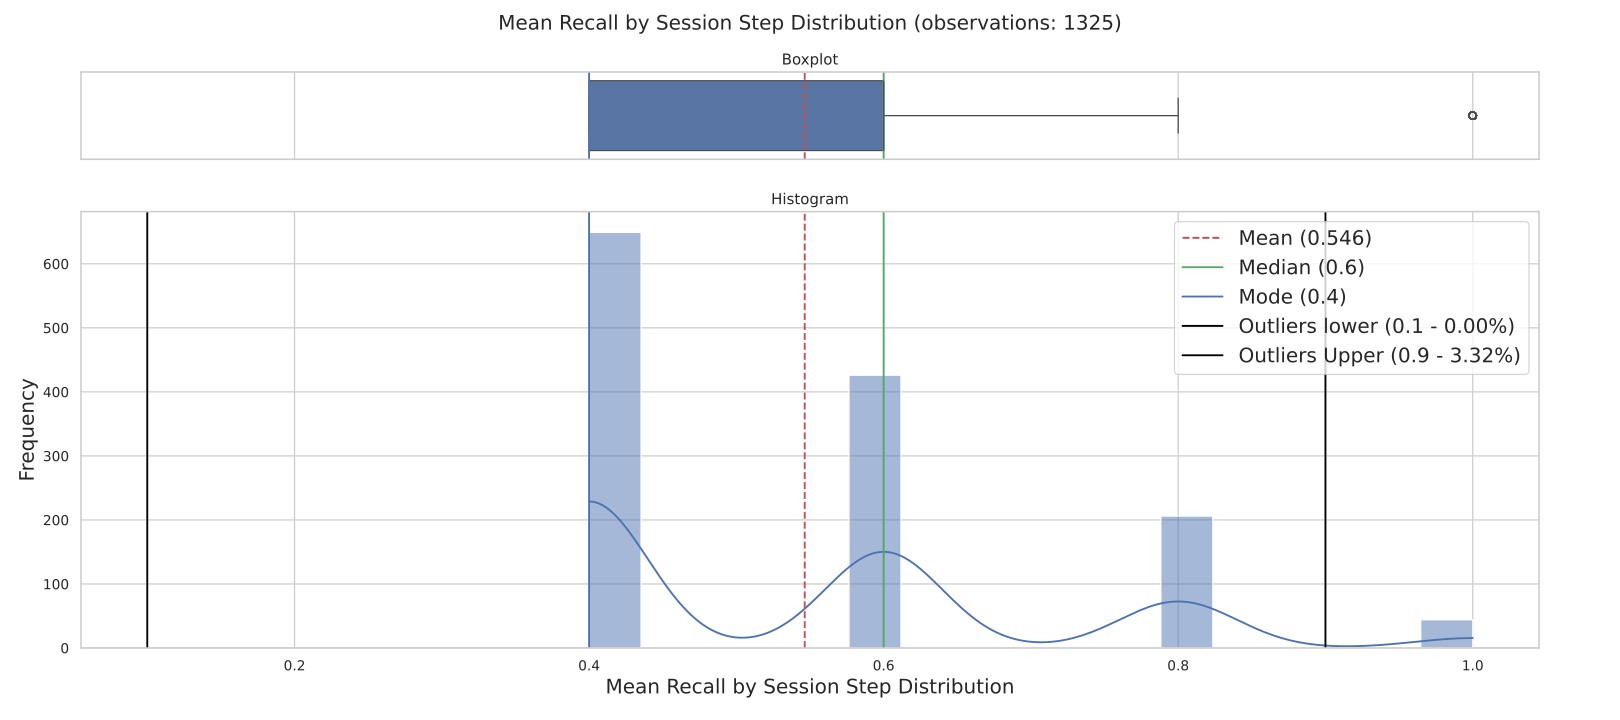
\includegraphics[width=15cm]{./images/llama3/mean_recall_by_session_step_distribution.png}
	\caption{Este gráfico muestra la distribución del \textit{Recall} promedio por paso (\textit{Session Step}).}
	\label{fig:llama3-mean_recall_by_session_step_distribution}
\end{figure}


En la figura \ref{fig:llama3-mean_recall_by_session_step_distribution} muestra la distribución del \textit{Recall} promedio que presenta $1325$ observaciones, con una media ligeramente menor a la obtenida al utilizar \textit{Llama2} de $0.546$ y la misma mediana de $0.6$ (ver figura \ref{fig:llama2-mean_recall_by_session_step_distribution}). También se mantiene la moda en $0.4$, pero muestra algunas diferencias notables con \textit{Llama2} en su distribución. Se observa la presencia de \textit{outliers} superiores (por encima de $0.9$) que representan el $3.32\%$ de las observaciones, y el límite inferior se establece en $0.1$, a diferencia del rango más amplio de \textit{LLama2}. \textit{LLama2} cuenta con más observaciones ($1419$ vs $1325$), lo que podría indicar una ligera diferencia en la cantidad de sesiones procesadas. Las medianas son idénticas ($0.6$) con ambos modelos. \textit{Llama2} muestra un rendimiento promedio ligeramente superior ($0.585$ vs $0.546$). Ambos mantienen la moda en $0.4$, indicando una consistencia en el comportamiento base. Ambos modelos presentan una distribución multimodal similar. \textit{LLama3} muestra una distribución más definida de los valores extremos, con \textit{outliers} claramente identificados. La concentración de valores alrededor de los picos principales es más pronunciada en \textit{LLama3}. Las diferencias del \textit{Recall} promedio por paso entre ambos modelos son sutiles. Al utilizar \textit{LLama2} se muestra un rendimiento promedio ligeramente superior, ya que con \textit{LLama3} los valores mas altos de la métricas son atípicos a diferencia
\textit{LLama2} don de esos mismo valores con mas probables.

\clearpage

En la figura \ref{fig:llama3-mean_recall_by_session_step_series} se muestra la evolución del \textit{Recall} promedio por paso (\textit{Session Step}).

\begin{figure}[H]
	\centering
	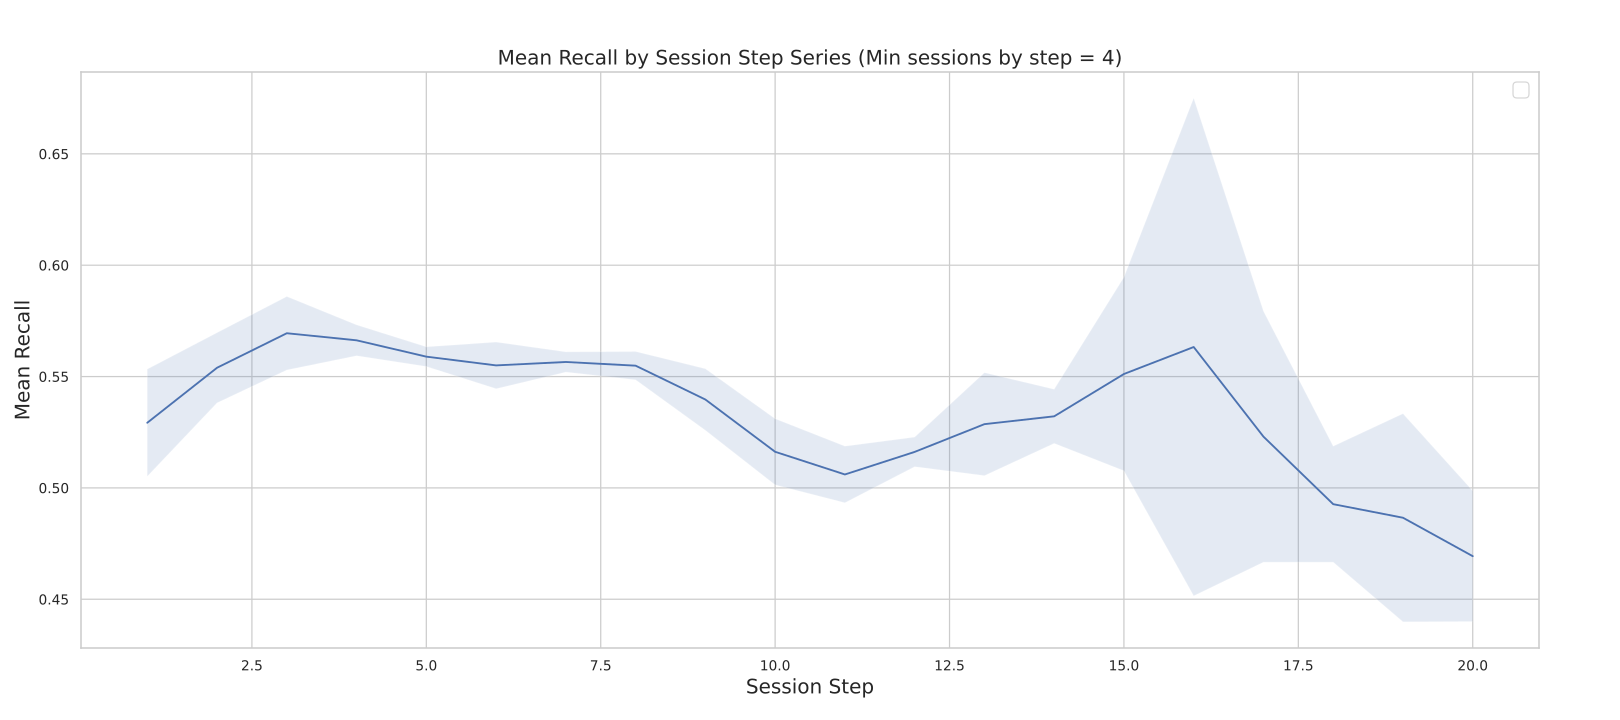
\includegraphics[width=15cm]{./images/llama3/mean_recall_by_session_step_series.png}
	\caption{En el gráfico se aprecia la evolución del \textit{Recall} promedio por paso (\textit{Session Step}).}
	\label{fig:llama3-mean_recall_by_session_step_series}
\end{figure}



En comparación con la figura \ref{fig:llama2-mean_recall_by_session_step_series}, se puede apreciar un comportamiento más estable, iniciando en $0.52$ y manteniendo valores entre $0.50-0.57$ hasta el paso $15$. Después, experimenta una caída similar al utilizar \textit{llama2} (figura \ref{fig:llama3-mean_recall_by_session_step_series}), pero con un intervalo de confianza más amplio entre los pasos $15-17$. Al utilizar \textit{Llama2} (figura \ref{fig:llama3-mean_recall_by_session_step_series}) la serie inicia con mejor rendimiento pero decae constantemente mientras que utilizando \textit{Llama3} se mantiene mayor estabilidad en pasos intermedios. Ambas series muestran deterioro después del paso $15$. Utilizando \textit{Llama3} se exhibe mayor variabilidad en intervalos de confianza. Ademas con \textit{Llama3} se muestra mejor capacidad para mantener el rendimiento en sesiones largas, aunque con mayor incertidumbre. La evolución sugiere que utilizar el componente \textit{Llama3} logra mayor estabilidad en el rendimiento a lo largo de la sesión, aunque sacrifica el \textit{Recall} inicial más alto que se muestra al utilizar el componente \textit{Llama2}.

\clearpage

En la figura \ref{fig:llama3-mean_reciprocal_rank_by_session_distribution} se muestra la distribución del \textit{Mean Reciprocal Rank (MRR)} por paso sesión.

\begin{figure}[H]
	\centering
	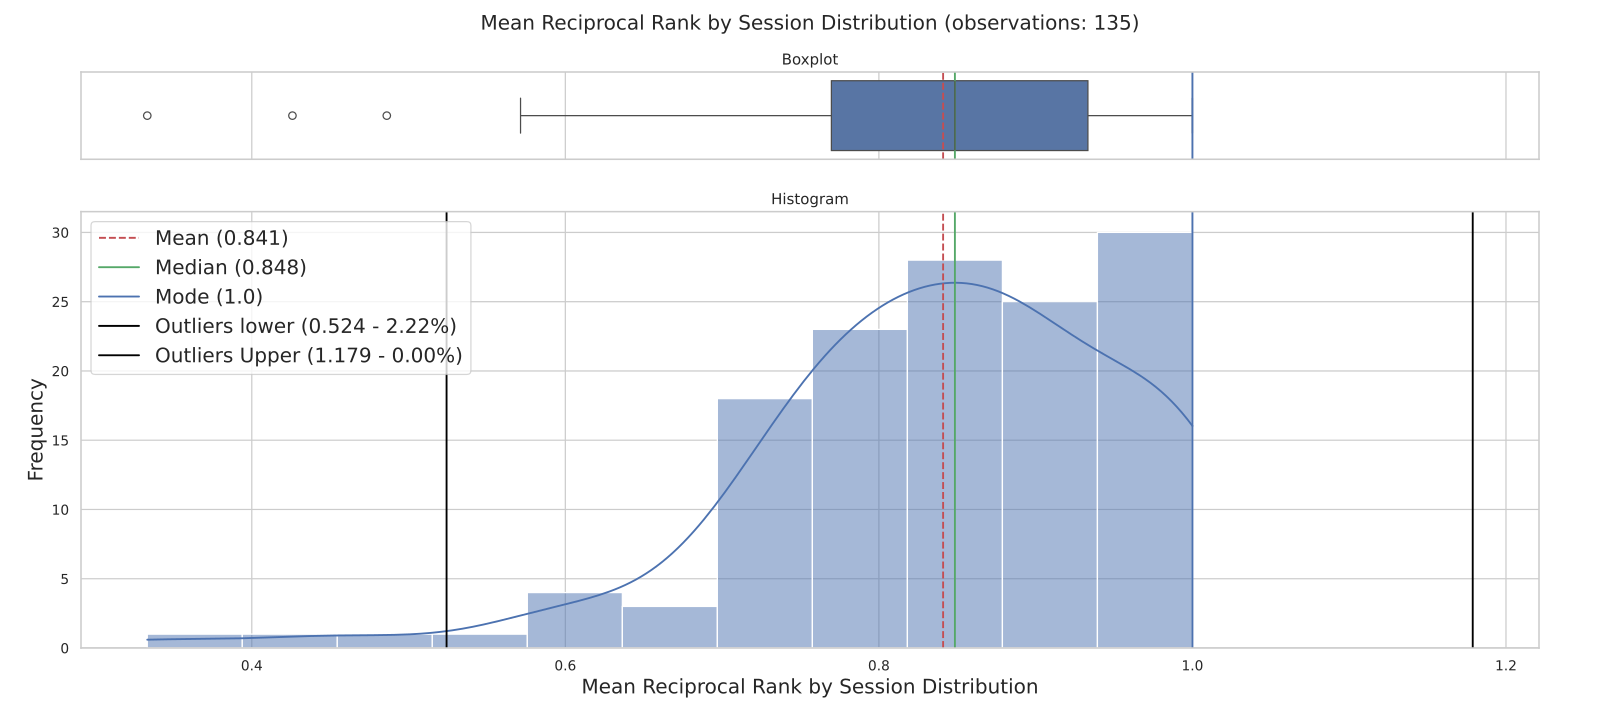
\includegraphics[width=15cm]{./images/llama3/mean_reciprocal_rank_by_session_distribution.png}
	\caption{En este gráfico se aprecia la distribución del \textit{Mean Reciprocal Rank (MRR)} por paso sesión.}
	\label{fig:llama3-mean_reciprocal_rank_by_session_distribution}
\end{figure}

En la figura \ref{fig:llama3-mean_reciprocal_rank_by_session_distribution}, al observar la distribución de los valores de \textit{Mean Reciprocal Rank (MRR)}, podemos deducir varias cosas sobre cómo se comporta el sistema de recomendación utilizando el componente \textit{Llama3}. En términos generales, al utilizar el \textit{Llama3} parece estar haciendo un trabajo bastante sólido. El valor promedio del \textit{Mean Reciprocal Rank (MRR)} indica que, en promedio, los elementos relevantes se encuentran relativamente cerca del principio de las listas de recomendaciones. Esto sugiere que el modelo está captando las preferencias de los usuarios con una precisión aceptable.
Sin embargo, la distribución de los valores no es completamente uniforme. se observa una cierta dispersión en los resultados, lo que indica que en algunos casos el sistema de recomendación funciona excepcionalmente bien, mientras que en otros su desempeño es menos destacado. Estos casos extremos (\textit{outliers},) podrían ser el resultado de factores como la complejidad de las preferencias del usuario, la calidad de los datos de entrenamiento o incluso errores aleatorios.
Un aspecto interesante es que el valor de \textit{Mean Reciprocal Rank (MRR)} más frecuente (la moda) es $1.0$. Esto significa que en una proporción significativa de las ocasiones, el sistema logra recomendar el elemento más relevante justo en la primera posición de la lista. Este es un resultado muy positivo y sugiere que el modelo está aprendiendo a captar las preferencias de los usuarios de manera efectiva.
Al comparar la distribución del \textit{Mean Reciprocal Rank (MRR)} utilizando ambos componentes \textit{Llama2} y \textit{Llama3}, podemos extraer las siguientes conclusiones clave: Al utilizar \textit{llama3} se tiende a mostrar un desempeño ligeramente superior en términos de \textit{MRR} promedio, lo que indica que, en general, sus recomendaciones son más precisas.
Utilizando \textit{Llama2} se presentar un mayor porcentaje de recomendaciones perfectas (\textit{MRR=1}), lo que podría ser crucial en aplicaciones donde la precisión absoluta es prioritaria. Ademas al utilizar \textit{Llama3}, suele mostrar una distribución más concentrada alrededor de la media, lo que sugiere un desempeño más consistente, con \textit{Llama2} puede presentar una mayor variabilidad en los resultados, con más casos extremos (\textit{outliers}).


\clearpage

En la figura \ref{fig:llama3-mean_reciprocal_rank_by_session_step_series} se muestra la evolución del \textit{Mean Reciprocal Rank (MRR)} por pasos de sesión.

\begin{figure}[H]
	\centering
	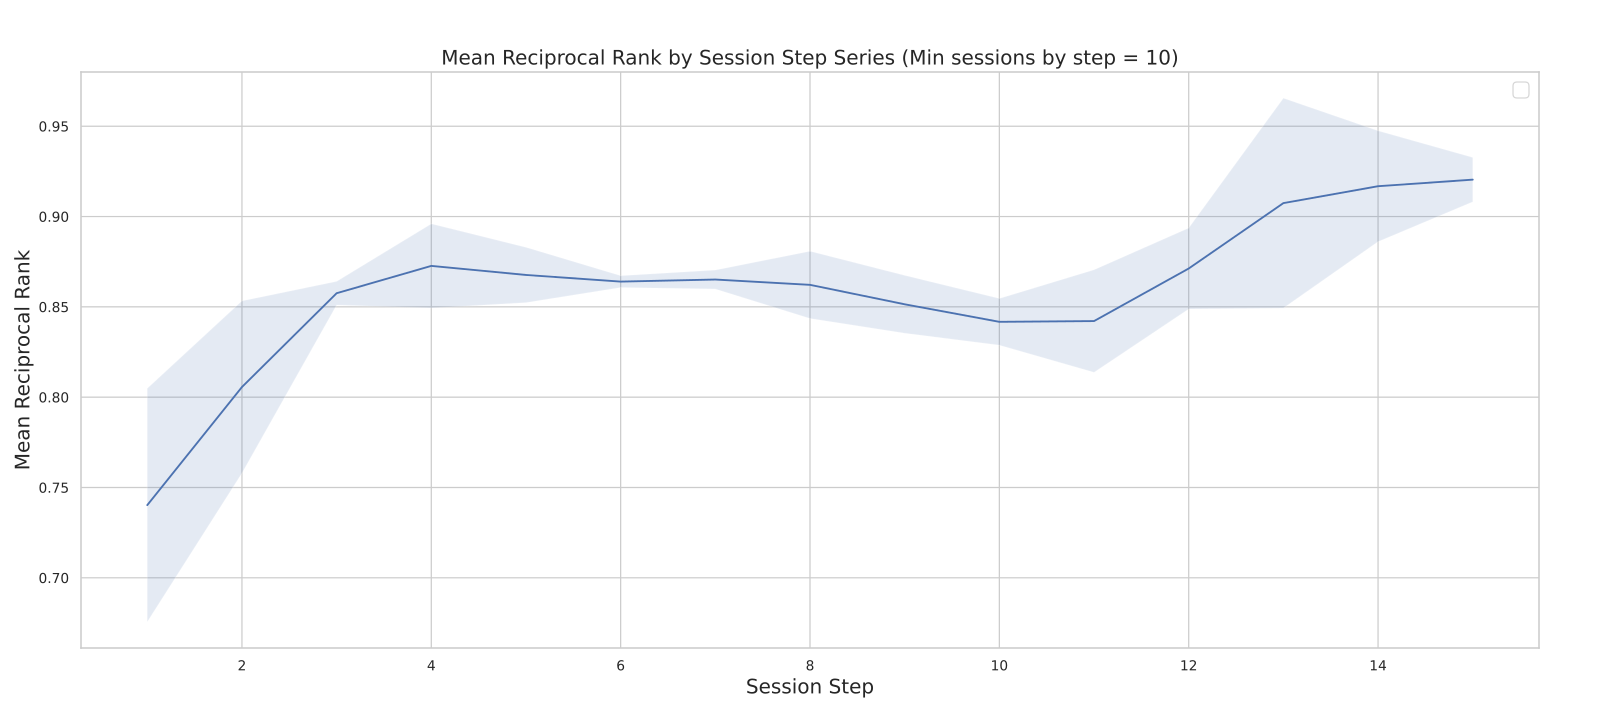
\includegraphics[width=15cm]{./images/llama3/mean_reciprocal_rank_by_session_step_series.png}
	\caption{En este gráfico se aprecia la evolución del \textit{Mean Reciprocal Rank (MRR)} por pasos de sesión.}
	\label{fig:llama3-mean_reciprocal_rank_by_session_step_series}
\end{figure}

En la figura \ref{fig:llama3-mean_reciprocal_rank_by_session_step_series} se aprecia que al inicio, el \textit{Mean Reciprocal Rank (MRR)} presenta una tendencia al alza, lo que indica que la calidad de las recomendaciones mejora a medida que el sistema de recomendación se expone a mas interacciones de los usuarios y aprende a ajustar mejor sus parámetros. A partir de cierto punto, el  \textit{Mean Reciprocal Rank (MRR)} se estabiliza y fluctúa alrededor de un valor promedio. Esto sugiere que el sistema de recomendación ha alcanzado un nivel de saturación en su aprendizaje. La zona sombreada indica que existe una cierta variabilidad en el \textit{Mean Reciprocal Rank (MRR)} a lo largo de las sesiones. Esto puede deberse a diferentes factores, como la complejidad de los datos, la diversidad de los usuarios o la naturaleza estocástica del proceso de aprendizaje.


\clearpage

En la figura \ref{fig:llama3-rated_items_by_session_distribution} se puede visualizar la distribución de la cantidad de ítems relevantes calificados por sesión de usuario.


\begin{figure}[H]
	\centering
	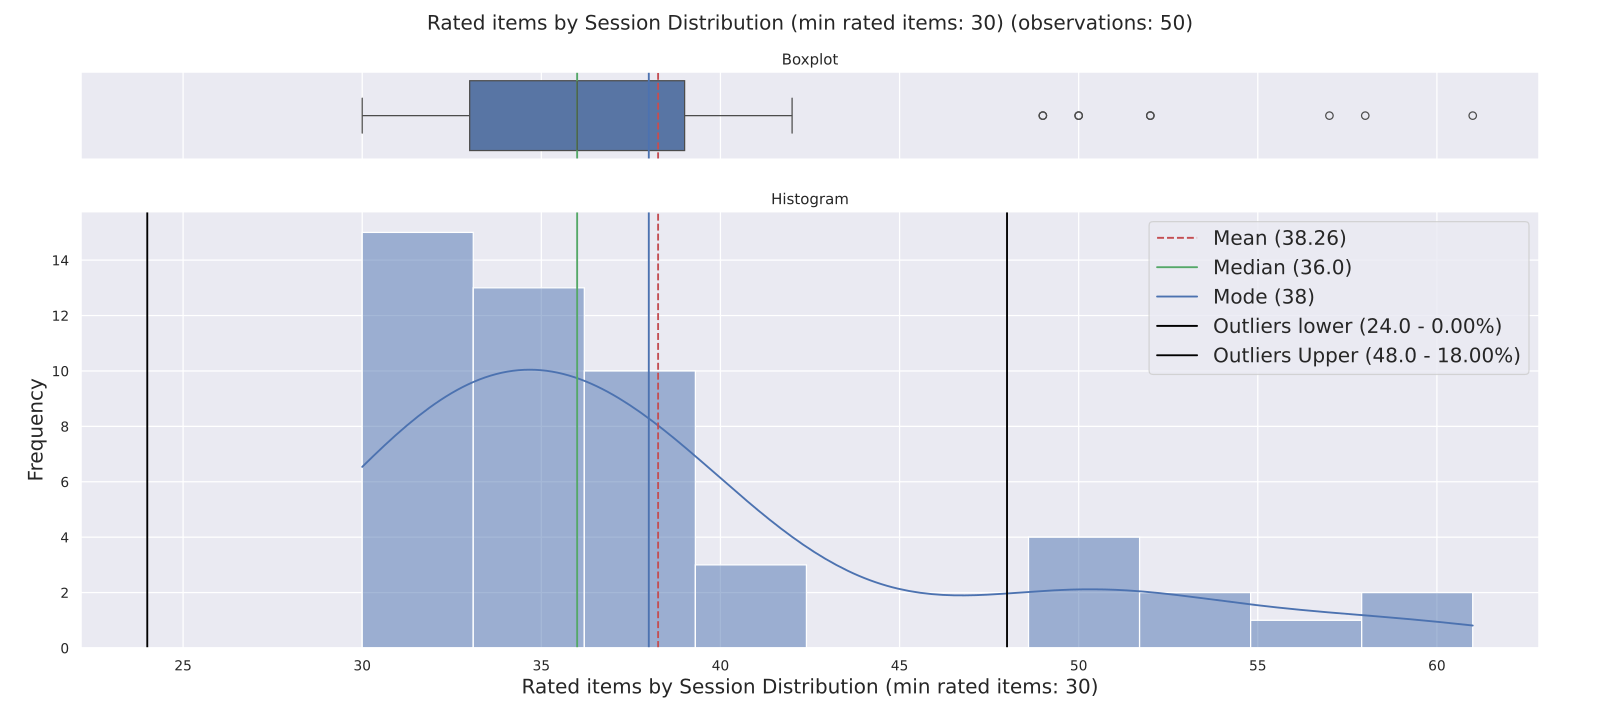
\includegraphics[width=15cm]{./images/llama3/rated_items_by_session_distribution.png}
	\caption{En este gráfico se puede visualizar la distribución de la cantidad de ítems relevantes calificados por sesión de usuario.}
	\label{fig:llama3-rated_items_by_session_distribution}
\end{figure}


La figura \ref{fig:llama3-rated_items_by_session_distribution} nos brinda una visión clara sobre la cantidad de ítems que, en promedio, los usuarios evalúan durante cada sesión. Cada punto de datos representa una sesión y el valor asociado indica el número total de ítems que el usuario ha calificado dentro de esa sesión. En promedio, los usuarios evalúan alrededor de $38$ ítems por sesión. Existe una considerable variabilidad en el número de ítems evaluados por sesión. Algunos usuarios evalúan un número significativamente mayor o menor de ítems en comparación con el promedio. Esta variabilidad puede deberse a diversos factores, como las características individuales de los usuarios, el tipo de contenido recomendado o el contexto en el que se realiza la evaluación. La distribución de los datos sugiere que la mayoría de las sesiones se concentran alrededor del valor promedio, con una ligera tendencia hacia la derecha. Esto indica que hay un mayor número de sesiones con una cantidad de ítems evaluados superior al promedio. Al comparar los resultados al utilizar los componentes \textit{Llama2} y \textit{Llama3} en cuanto a la cantidad de ítems calificados por sesión, podemos observar algunas diferencias significativas: \textit{Llama2} tiende a generar una mayor cantidad de recomendaciones relevantes por sesión. Esto sugiere que este modelo es más eficaz a la hora de identificar los intereses de los usuarios y presentarles contenido que consideran valioso. Sin embargo, esta mayor cantidad de recomendaciones viene acompañada de una mayor variabilidad en los resultados, lo que significa que la calidad de las recomendaciones puede fluctuar más de un usuario a otro. \textit{Llama3} presenta resultados más consistentes. La cantidad de ítems calificados por sesión es menos variable, lo que indica que la calidad de las recomendaciones es más estable. No obstante, el número promedio de recomendaciones relevantes es ligeramente inferior en comparación con \textit{Llama2}.


\clearpage

En la figura \ref{fig:llama3-relevant_items_found_by_step_index_for_all_sessions} se muestra el número de ítems relevantes encontrados en cada paso para todas las sesiones de usuario, segmentado por la cantidad de ítems relevantes en las
respuestas del sistemas de recomendación.

\begin{figure}[H]
	\centering
	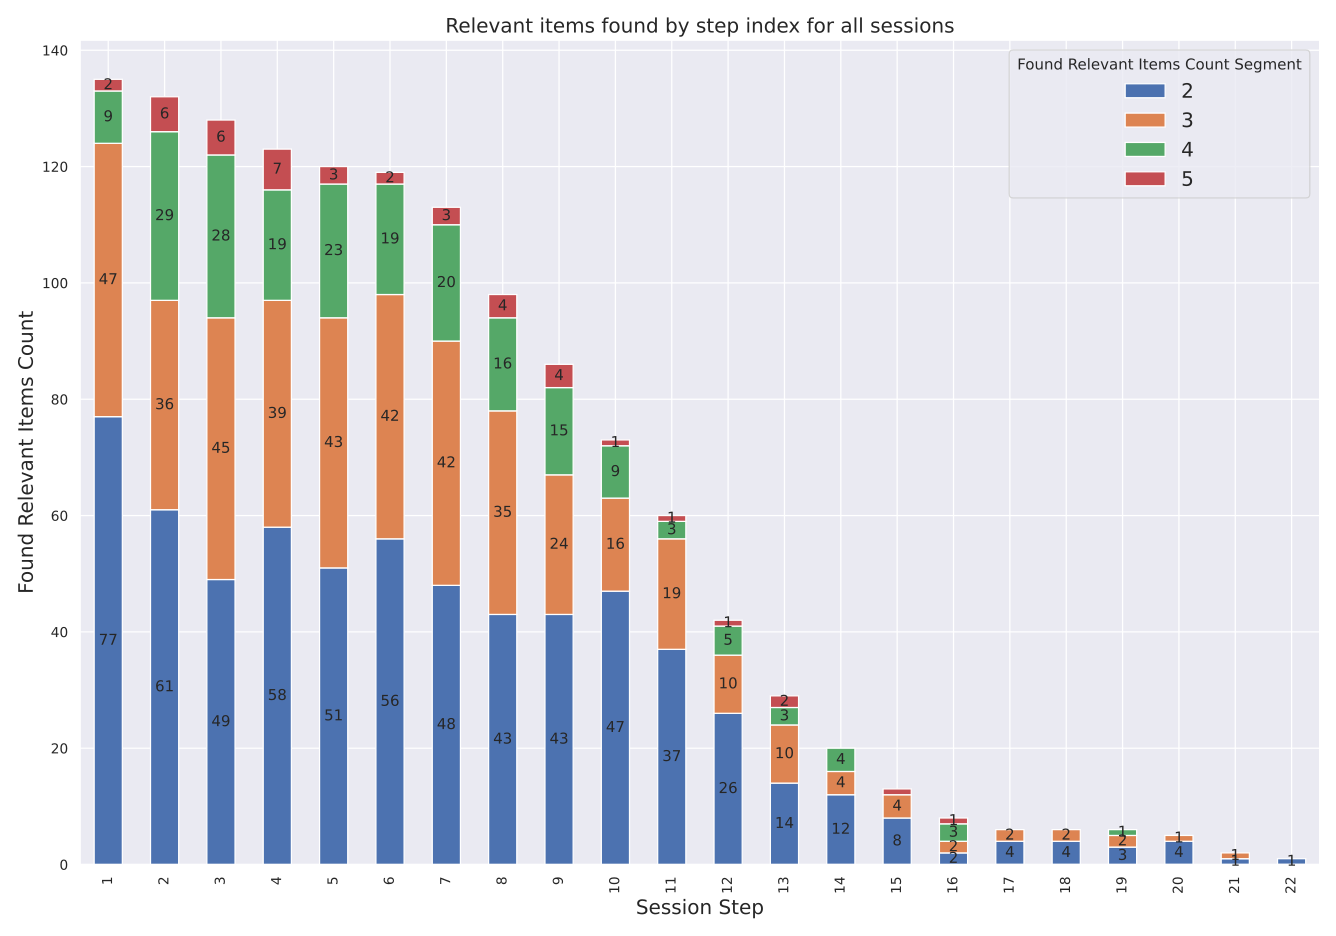
\includegraphics[width=15cm]{./images/llama3/relevant_items_found_by_step_index_for_all_sessions.png}
	\caption{En este gráfico se puede apreciar el número de ítems relevantes encontrados en cada paso
		para todas las sesiones de usuario, segmentado por la cantidad de ítems relevantes en
		las respuestas del sistemas de recomendación.}
	\label{fig:llama3-relevant_items_found_by_step_index_for_all_sessions}
\end{figure}


En la figura \ref{fig:llama3-relevant_items_found_by_step_index_for_all_sessions} se observa una disminución en la cantidad de ítems relevantes a medida que avanza la sesión. Esto podría indicar que el sistema es más efectivo en encontrar ítems relevantes al inicio de la sesión, y que a medida que se exploran más opciones, la relevancia de las recomendaciones puede disminuir. Existe una gran variabilidad entre las diferentes sesiones. Algunas sesiones logran encontrar una gran cantidad de ítems relevantes en los primeros pasos, mientras que otras mantienen un nivel más constante a lo largo de toda la sesión. La cantidad de ítems relevantes encontrados parece estar influenciada por el paso de la sesión. En los primeros pasos, se suelen encontrar más ítems relevantes, mientras que en los últimos pasos la cantidad tiende a disminuir.
Al utilizar \textit{Llama2} se muestra una mayor consistencia en sus recomendaciones, lo que se traduce en una menor variabilidad entre sesiones. Esto sugiere que \textit{Llama2} es más confiable a la hora de proporcionar resultados similares para diferentes usuarios en situaciones similares. Sin embargo, podría ser que \textit{Llama3} sea más innovador y capaz de sugerir ítems más sorpresivos o menos convencionales, aunque con una mayor tasa de aciertos y fallos.
\textit{Llama3}, por su parte, podría destacar en la capacidad de adaptarse rápidamente a las preferencias del usuario, alcanzando un pico de relevancia más temprano en la sesión. Esto indica que \textit{Llama3} podría ser más eficaz en captar los intereses iniciales del usuario. No obstante, esta rapidez en la adaptación podría venir acompañada de una mayor tasa de falsos positivos en etapas posteriores de la sesión.


\chapter{Comparación de resultados}

Al comparar el modelo de recomendación utilizando los componentes \textit{llama2} y \textit{llama3}, se observan ciertas diferencias:

\begin{itemize}
	\item \textit{Normalized Discounted Cumulative Gain (NDCG)}: Ambos componentes presentan diferencias mínimas. La mayoría de las sesiones logran un rendimiento óptimo en el posicionamiento de items relevantes. Ambas distribuciones tienen una cola izquierda que se extiende hacia valores bajos, con una notable concentración de observaciones entre el $95\%$ y el $100\%$. El \textit{boxplot} refleja una distribución compacta en el rango inter-cuantil, lo que sugiere alta consistencia en el rendimiento del sistema para la mayoría de las sesiones. Por otro lado, en la evolución del \textit{NDCG}, \textit{LLama3} muestra una mayor estabilidad general, con fluctuaciones menos pronunciadas a diferencia de \textit{LLama2}. Esto sugiere una mejor gestión en la transición entre diferentes estrategias de recomendación. Mientras que al utilizar \textit{LLama2} se muestra una tendencia descendente en los pasos finales, \textit{LLama3} mantiene una tendencia ascendente, indicando una mejor capacidad para mantener la calidad de las recomendaciones en sesiones más largas.

	\item \textit{Mean Average Precision} (\textit{MAP}): Al emplear el modelo con el componente \textit{Llama3}, se observa una mayor precisión en el posicionamiento de ítems relevantes en las primeras posiciones. Para esta métrica, los ítems relevantes son aquellos calificados por el usuario entre 4 y 5 puntos.
	      Por otro lado, si observamos la evolución temporal de \textit{Mean Average Precision} (\textit{MAP}) vemos patrones casi opuestos. Mientras que el modelo con \textit{Llama2} exhibe una degradación gradual desde un punto inicial alto, el modelo con \textit{Llama 3} se mantiene siempre por debajo de \textit{Llama 2} pero con un comportamiento mas estable. \textit{Mean Average Precision} (\textit{MAP}) es una métrica más estricta en términos de puntuación en comparación a \textit{Normalized Discounted Cumulative Gain (NDCG)}, donde solo se considera el orden de los ítems sin requerir un mínimo en su puntuación. Se puede decir que \textit{MAP} y \textit{NDGC} son métricas complementarias en esta área de evaluación.

	\item \textit{Mean Reciprocal Rank (MRR)}: Al utilizar \textit{llama3} se tiende a mostrar un desempeño. ligeramente superior en términos de \textit{MRR} promedio, lo que indica que, en general, sus recomendaciones son más precisas. Ademas al utilizar \textit{Llama3}, se puedo visualizar una distribución más concentrada alrededor de la media, lo que sugiere un desempeño más consistente, con \textit{Llama2} se presenta una mayor variabilidad en los resultados, con más casos extremos (\textit{outliers}).

	\item Recall: Al observar la distribución del Recall promedio por paso, las diferencias entre ambos modelos son sutiles. Al utilizar LLama2 se muestra un rendimiento ligeramente superior, ya que con LLama3 los valores mas altos de la métricas son atípicos a diferencia de LLama2, donde esos mismo valores son mas probables. En cuanto a la evolución por paso, con llama3 se puede apreciar un comportamiento más estable. Al utilizar Llama2 la serie inicia con mejor rendimiento pero decae constantemente, mientras que utilizando Llama3 se mantiene mayor estabilidad en pasos intermedios. La evolución sugiere que utilizar el componente Llama3 logra mayor estabilidad en el rendimiento a lo largo de las sesiones.

	\item Cantidad de ítems relevantes por paso: Al utilizar ambos modelos, se observa una gran variabilidad entre las sesiones. Algunas logran identificar más ítems relevantes en los primeros pasos, mientras que otras mantienen un nivel más constante a lo largo de la sesión. A medida que avanzan los pasos, la cantidad de ítems relevantes tiende a disminuir.

	      El modelo Llama2 muestra menos dificultad para encontrar ítems relevantes en comparación con Llama3. A lo largo de las sesiones, Llama2 logra identificar más resultados con 4 y 5 ítems relevantes. No se observan diferencias significativas con 2 y 3 ítems, ya que ambos modelos presentan cantidades similares por paso. Aunque las diferencias son muy sutiles, parece que Llama2 tiene menos dificultades para encontrar ítems relevantes.

\end{itemize}

Se observa que una opción viable seria utilizar el componente \textit{llama3}, ya que presenta una tendencia más estable en términos de \textit{NDGC}. Además, muestra mayor precisión en términos del \textit{MAP} y \textit{MRR} promedio. Aunque no hay grandes diferencias en Recall y en la cantidad de ítems relevantes, se puede notar que \textit{llama2} tiene un mayor recall promedio, evidenciado por un mayor número de resultados con 4 y 5 ítems relevantes. La elección entre modelos dependerá de la prioridad al recomendar ítems; un modelo con menor recall también ofrece más oportunidades de descubrir nuevo contenido similar. Desde esta perspectiva, \textit{llama3} podría ser un mejor candidato. Sin embargo, \textit{llama2} no tiene un recall perfecto y enfrenta el mismo desafío.

\chapter{Conclusiones}

En este trabajo se exploró el uso de grandes modelos de lenguaje en sistemas de recomendación, analizando su impacto en la personalización de contenidos y la experiencia del usuario \cite{chatrec}. A través de la integración de técnicas como \textit{Retrieval-Augmented Generation (RAG)} ~\cite{rag} y filtros colaborativos, se logró mejorar la capacidad del sistema para ofrecer recomendaciones adaptadas a las preferencias de cada usuario.

Uno de los principales hallazgos fue la limitación en la memoria de los grandes modelos de lenguaje locales, lo que afectó la capacidad de recordar interacciones previas y generar recomendaciones consistentes. Asimismo, se identificaron problemas en la aleatoriedad de los modelos, que en algunas instancias generaban respuestas con estructuras inconsistentes, lo que requirió el desarrollo de \textit{parsers} especializados.

En términos de eficiencia computacional, se constató que el tiempo de inferencia de los grande modelos de lenguaje locales es significativamente mayor en comparación con soluciones en la nube como \textit{Claude AI} o \textit{ChatGPT-4o } de \textit{Open AI}. Esto plantea un desafío en la escalabilidad del sistema, ya que el costo de los recursos computacionales podría volverse prohibitivo a gran escala.

El problema de \textit{Cold Start} o arranque en frio, característico de los sistemas de recomendación, se abordó mediante la utilización de \textit{embeddings} utilizando la técnica \textit{RAG}(\textit{Retrieval Augmented Generation} o Generación Aumentada por Recuperación) ~\cite{rag} , permitiendo mejorar la calidad de las recomendaciones iniciales sin requerir interacciones previas del usuario. No obstante, se observó que, con el tiempo, la relevancia del contenido recomendado disminuye a medida que se agotan los elementos más relevantes dentro del catálogo disponible.

Como parte del \textit{pipeline} de entrenamiento y actualización de modelos, se utilizó \textit{Apache Airflow} ~\cite{apache-airflow} para orquestar los flujos de datos y garantizar la actualización continua de \textit{embeddings} y modelos de recomendación. Este enfoque demostró ser eficiente para manejar grandes volúmenes de datos y asegurar la disponibilidad de modelos actualizados.

En futuras investigaciones, se planea explorar modelos híbridos que combinen la eficiencia de los grandes modelos de lenguaje  locales con la capacidad de procesamiento de modelos en la nube, así como optimizar técnicas de \textit{prompt engineering} para mejorar la interpretabilidad de las respuestas generadas por los grandes modelos de lenguaje. Además, podría analizarse la incorporación de estrategias de aprendizaje continuo (\textit{ Continual Learning o Lifelong Learning}) que permitan adaptar las recomendaciones de manera dinámica según la evolución de las preferencias del usuario.

Este trabajo contribuye al estudio de la aplicación de modelos de lenguaje en sistemas de recomendación, destacando tanto sus beneficios como sus limitaciones y estableciendo una base para futuras optimizaciones en este campo.


\chapter{Glosario}

\begin{description}

	\item[Filtrado Colaborativo]: Método de recomendación que se basa en las preferencias y comportamientos de múltiples usuarios para sugerir ítems. Se divide en dos enfoques: basado en usuarios y basado en ítems.
	\item[Recomendación Basada en Contenido]: Técnica que sugiere ítems similares a aquellos que el usuario ha mostrado interés previamente, utilizando las características del contenido.
	\item[Modelos Híbridos]: Sistemas de recomendación que combinan múltiples técnicas, como filtrado colaborativo y basado en contenido, para mejorar la precisión de las sugerencias.
	\item[Retroalimentación Implícita]: Datos obtenidos indirectamente sobre las preferencias del usuario, como clics, tiempo de visualización o historial de navegación, en contraste con la retroalimentación explícita como calificaciones o reseñas.
	\item[Recomendación Basada en Contexto]: Método que tiene en cuenta el contexto del usuario, como ubicación, hora del día o dispositivo utilizado, para ofrecer sugerencias más relevantes.
	\item[Serendipia (Serendipity)]: Métrica que evalúa la capacidad del sistema para sorprender al usuario con recomendaciones inesperadas pero relevantes.
	\item[Sistemas de Recomendación Basados en Popularidad]: Método que sugiere ítems que son populares entre todos los usuarios, sin personalización individual.
	\item[Filtrado Basado en Conocimiento]: Técnica que utiliza información específica sobre los ítems y las necesidades del usuario para realizar recomendaciones.
	\item[Sistemas de Recomendación Basados en Redes Neuronales]: Modelos que emplean redes neuronales para capturar relaciones complejas entre usuarios e ítems y mejorar las recomendaciones.
	\item[LLM (Large Language Models)]: Modelos de lenguaje de gran escala entrenados con grandes volúmenes de datos para comprender y generar texto de manera sofisticada.
	\item[Retrieval-Augmented Generation (RAG)]: Técnica que combina recuperación de información y generación de texto para mejorar la precisión y relevancia de las respuestas generadas por modelos de lenguaje.
	\item[Cold Start]: Problema en los sistemas de recomendación que ocurre cuando no hay suficiente información sobre un usuario o ítem para generar recomendaciones precisas.
	\item[Embeddings]: Representaciones vectoriales de palabras, frases o elementos de datos que permiten medir similitudes en un espacio continuo.
	\item[DeepFM]: Modelo basado en redes neuronales profundas y factorization machines para mejorar la predicción en sistemas de recomendación.
	\item[Apache Airflow]: Plataforma de orquestación de flujos de trabajo utilizada para programar, gestionar y monitorear procesos de datos.
	\item[Prompt Engineering]: Técnica para diseñar instrucciones o entradas optimizadas que mejoran la calidad de las respuestas de modelos de lenguaje.
	\item[Aprendizaje Continuo]: Estrategia de machine learning en la que un modelo se actualiza dinámicamente con nuevos datos sin necesidad de ser re-entrenado completamente desde cero.
	\item[Factorization Machines (FM)]: Algoritmo utilizado en sistemas de recomendación para modelar interacciones entre variables categóricas y continuas.
	\item[Transfer Learning]: Técnica de aprendizaje automático en la que un modelo pre-entrenado en un dominio se ajusta a un nuevo dominio con menos datos.
	\item[NDCG (Normalized Discounted Cumulative Gain)]: Métrica utilizada para evaluar la calidad de las recomendaciones basadas en la relevancia y el orden de los ítems recomendados.
	\item[MAP (Mean Average Precision)]: Promedio de las precisiones obtenidas en cada consulta en un sistema de recomendación.
	\item[MRR (Mean Reciprocal Rank)]: Promedio del recíproco de la posición del primer resultado relevante en una lista de recomendaciones.
	\item[ChromaDB] Base de datos orientada a almacenamiento de embeddings utilizada para búsqueda de similitud en recomendaciones.
\end{description}


\printbibliography[title=Referencias]

\end{document}